\documentclass[a4paper,12pt,twoside]{report}

\usepackage{fontspec}
\usepackage{xunicode}
\usepackage{xltxtra}
\usepackage{xgreek}
\usepackage{csquotes}
\usepackage{placeins}

\raggedbottom
\onecolumn

\usepackage{graphicx,amsfonts,psfrag,fancyhdr,layout,subfigure}
\usepackage{multirow}
\usepackage{longtable}
\usepackage{array}

\usepackage[toc,page]{appendix}
\renewcommand{\appendixtocname}{Παραρτήματα}
\renewcommand{\appendixname}{Παράρτημα}
\renewcommand{\appendixpagename}{Παραρτήματα}

\setmainfont[Mapping=tex-text]{GFS Artemisia}

\usepackage[style=numeric, bibstyle=numeric, hyperref=true, backref=true, alldates=terse, indexing=false, backend=bibtex]{biblatex}
\addbibresource{Bibliography.bib}

\usepackage{index}
\usepackage[columns=2]{idxlayout}
\newindex{default}{idx}{ind}{Ευρετήριο}

\usepackage{hyperref}

\usepackage[acronym, toc, translate=true]{glossaries}
\newglossary[trt]{translatedTerms}{trr}{trn}{Λεξικό αγγλικών όρων}
\loadglsentries{acronyms.tex}
\loadglsentries{glossary.tex}
\loadglsentries[translatedTerms]{translatedTerms.tex}
\renewcommand{\glossaryname}{Γλωσσάρι}
\renewcommand{\acronymname}{Συντομογραφίες}
\makeglossaries

% Set equal margins on book style
\setlength{\oddsidemargin}{53pt}
\setlength{\evensidemargin}{53pt}
\setlength{\marginparwidth}{57pt}
\setlength{\footskip}{30pt}

%%%%%%%%%%%%%%%%%%%%%%%%%%%%%%%%%%%%%%%%%%%%%%%%%%%%%%%%%%%%%
%%%%%%%%%%%%%%		   								Παράμετροι	   					   %%%%%%%%%%%%%%%%%%%%
%%%%%%%%%%%%%%%%%%%%%%%%%%%%%%%%%%%%%%%%%%%%%%%%%%%%%%%%%%%%%
\newcommand{ \FirstName}{ΔΗΜΗΤΡΙΟΣ ΑΝΔΡΕΑΣ }
\newcommand{ \LastName}{ΚΑΦΕΤΖΗΣ}
\newcommand{ \FathersName}{ΚΩΝΣΤΑΝΤΙΝΟΥ}
\newcommand{ \AM}{5657}
\newcommand{ \ThesisTitle}{ΑΞΙΟΛΟΓΗΣΗ ΤΗΣ ΓΛΩΣΣΑΣ ΜΟΝΤΕΛΟΠΟΙΗΣΗΣ ΣΥΣΤΗΜΑΤΩΝ SysML ΣΤΗΝ ΑΝΑΠΤΥΞΗ ΕΝΣΩΜΑΤΩΜΕΝΩΝ ΣΥΣΤΗΜΑΤΩΝ}
\newcommand{ \FirstProfessor}{ΚΛΕΑΝΘΗΣ ΘΡΑΜΠΟΥΛΙΔΗΣ}
\newcommand{ \FirstProfessorsRank}{ΚΑΘΗΓΗΤΗΣ}
\newcommand{ \SecondProfessor}{ΚΛΕΑΝΘΗΣ ΘΡΑΜΠΟΥΛΙΔΗΣ}
\newcommand{ \SecondProfessorsRank}{ΚΑΘΗΓΗΤΗΣ}
\newcommand{ \ThesisNumber}{ΧΧΧ}
\newcommand{ \ExaminationDay}{x}
\newcommand{ \ExaminationMonth}{x}
\newcommand{ \ExaminationYear}{x}
\newcommand{ \Month}{Απρίλιος}
\newcommand{ \Year}{2011}

% Document starts here
\begin{document}

% Page numberin set to arabic
\pagenumbering{roman}
%%%%%%%%%%%%%%%%%%%%%%%%%%%%%%%%%%%%%%%%%%%%%%%%%%%%%%%%%%%%%
%%%%%%%%%%%%%%		   								 Πρώτη σελίδα  					   %%%%%%%%%%%%%%%%%%%%
%%%%%%%%%%%%%%%%%%%%%%%%%%%%%%%%%%%%%%%%%%%%%%%%%%%%%%%%%%%%%
%%%%%%%%%%%%%%%%%%%%%%%%%%%%%%%%%%%%%%%%%%%%%%%%%%%%%%%%%%%%%
	{\label{Πρώτη σελίδα} 
		\newpage
		\begin{flushleft}
			\textbf{
				{\large ΠΑΝΕΠΙΣΤΗΜΙΟ ΠΑΤΡΩΝ} \linebreak
				{\normalsize ΤΜΗΜΑ ΗΛΕΚΤΡΟΛΟΓΩΝ ΜΗΧΑΝΙΚΩΝ \linebreak ΚΑΙ ΤΕΧΝΟΛΟΓΙΑΣ ΥΠΟΛΟΓΙΣΤΩΝ}\linebreak
				{\small ΤΟΜΕΑΣ:}\linebreak
				{\footnotesize ΕΡΓΑΣΤΗΡΙΟ }
			}
		\end{flushleft}
		\hrulefill
	
		\begin{center}
			\textbf{{\LARGE Διπλωματική Εργασία}}\linebreak
			{\large του φοιτητή του Τμήματος Ηλεκτρολόγων Μηχανικών και\linebreak 	Τεχνολογίας Υπολογιστών της Πολυτεχνικής Σχολής του \linebreak Πανεπιστημίου Πατρών}
			\linebreak \linebreak \linebreak
			{\large  \FirstName του \FathersName}
			\linebreak \linebreak
			{\large Αριθμός Μητρώου:\linebreak \AM}
			\linebreak \linebreak  \linebreak
			{\large \underline{Θέμα}}
			\linebreak  \linebreak
			{\Large \textbf{ \ThesisTitle}}
			\linebreak \linebreak \linebreak
			{\large \underline{Επιβλέπων}}
			\linebreak  \linebreak
			{\large \FirstProfessor}
			\linebreak \linebreak \linebreak \linebreak
			{\large \textbf{Αριθμός Διπλωματικής Εργασίας:\linebreak \ThesisNumber}}
			\linebreak \linebreak
			{\large Πάτρα, \Month \hspace{1pt} \Year}
		\end{center}
	}
 
%%%%%%%%%%%%%%%%%%%%%%%%%%%%%%%%%%%%%%%%%%%%%%%%%%%%%%%%%%%%%
%%%%%%%%%%%%%%		   								 Δεύτερη σελίδα					   %%%%%%%%%%%%%%%%%%%%
%%%%%%%%%%%%%%%%%%%%%%%%%%%%%%%%%%%%%%%%%%%%%%%%%%%%%%%%%%%%%
%%%%%%%%%%%%%%%%%%%%%%%%%%%%%%%%%%%%%%%%%%%%%%%%%%%%%%%%%%%%%
	{\label{Δεύτερη σελίδα} 
		\newpage
		\begin{center}
			\textbf{{\LARGE ΠΙΣΤΟΠΟΙΗΣΗ}}\linebreak \linebreak
			{\large Πιστοποιείται ότι η Διπλωματική Εργασία με θέμα}\linebreak \linebreak
			{\Large \textbf{ \ThesisTitle}}\linebreak\linebreak\linebreak
			\begin{large}
				Του φοιτητή του Τμήματος Ηλεκτρολόγων Μηχανικών και Τεχνολογίας Υπολογιστών\linebreak \linebreak \linebreak \FirstName \LastName  του \FathersName\linebreak \linebreak Αριθμός Μητρώου:  \linebreak \AM \linebreak \linebreak \linebreak Παρουσιάστηκε δημόσια και εξετάστηκε στο Τμήμα Ηλεκτρολόγων Μηχανικών και Τεχνολογίας Υπολογιστών στις \linebreak \ExaminationDay / \ExaminationMonth / \ExaminationYear \linebreak
			\end{large}
		\end{center}
		\vspace{3cm}
		\begin{large}
			\begin{tabular}{m{5cm} m{1cm} m{6cm}}
			Ο Επιβλέπων & & Ο Διευθυντής του Τομέα\\
			\FirstProfessor & & \SecondProfessor \\
			\FirstProfessorsRank & & \SecondProfessorsRank
			\end{tabular}
		\end{large}
	}
		
%%%%%%%%%%%%%%%%%%%%%%%%%%%%%%%%%%%%%%%%%%%%%%%%%%%%%%%%%%%%%
%%%%%%%%%%%%%%		   								 Τρίτη σελίδα  					   %%%%%%%%%%%%%%%%%%%%
%%%%%%%%%%%%%%%%%%%%%%%%%%%%%%%%%%%%%%%%%%%%%%%%%%%%%%%%%%%%%
%%%%%%%%%%%%%%%%%%%%%%%%%%%%%%%%%%%%%%%%%%%%%%%%%%%%%%%%%%%%%
	{\label{Τρίτη σελίδα} 
		\newpage
		\begin{large}
			\begin{flushleft}
				\textbf{Αριθμός Διπλωματικής Εργασίας:}\linebreak \linebreak
				\textbf{Θέμα: \ThesisTitle} \linebreak \linebreak
			\end{flushleft}
			\begin{tabular}{p{6cm} p{1cm} p{6cm}}
				Φοιτητής: & & Επιβλέπων:\\
				\FirstName \LastName & & \FirstProfessor\\
			\end{tabular}
			\linebreak \linebreak
			\begin{flushleft}\underline{{\large Περίληψη}}	\end{flushleft}
			\paragraph{} {
				ηγψξγηξηγξγηκξ
				}
		\end{large}
	}
		
\newpage
% Page numberin set to arabic
\pagenumbering{arabic}

% Remove parskip for toc
\setlength{\parskip}{0ex plus 0.5ex minus 0.2ex}
\tableofcontents

\listoffigures
\addcontentsline{toc}{chapter}{Κατάλογος Σχημάτων}

\listoftables
\addcontentsline{toc}{chapter}{Κατάλογος Πινάκων}



% Dutch style of paragraph formatting, i.e. no indents.
\setlength{\parskip}{1.3ex plus 0.2ex minus 0.2ex}

% Redefine plain page style
\fancypagestyle{plain}{
	\fancyhf{}
	\renewcommand{\headrulewidth}{0pt}
	\fancyfoot[LE,RO]{\thepage}
}

% Code for creating empty pages
% No headers on empty pages before new chapter
\makeatletter
	\def\cleardoublepage{
		\clearpage\if@twoside \ifodd\c@page\else
	    \hbox{}
	    \thispagestyle{plain}
	    \newpage
    	\if@twocolumn\hbox{}\newpage\fi\fi\fi
    }
\makeatother \clearpage{\pagestyle{plain}\cleardoublepage}

% Define pagestyle
\pagestyle{fancy}
\fancyhf{}
\renewcommand{\chaptermark}[1]{\markboth{ \emph{#1}}{}}

% Adjustments headers
\fancyhead[LO]{\emph{Κεφάλαιο \thechapter}}
\fancyhead[RE]{\leftmark}
\fancyfoot[LE,RO]{\thepage}

%%%%%%%%%%%%%%%%%%%%%%%%%%%%%%%%%%%%%%%%%%%%%%%%%%%%%%%%%%%%%
%%%%%%%%%%%%%%		   								 Κεφάλαιο		   					   %%%%%%%%%%%%%%%%%%%%
%%%%%%%%%%%%%%%%%%%%%%%%%%%%%%%%%%%%%%%%%%%%%%%%%%%%%%%%%%%%%
%%%%%%%%%%%%%%%%%%%%%%%%%%%%%%%%%%%%%%%%%%%%%%%%%%%%%%%%%%%%%
	\newpage
	\addcontentsline{toc}{chapter}{Πρόλογος}
	\chapter*{Πρόλογος}
	
		\paragraph{}{Ειαγωγή********************************************************
		}
		
		\paragraph{Κεφάλαιο \ref{κεφ.:Σύστημα και ενσωματωμένα συστήματα}} {Αναλύεται η έννοια του συστήματος και το επιστημονικό πεδίο των ενσωματωμένων συστημάτων. Εισάγονται βασικές έννοιες και δίδονται θεμελιώδεις ορισμοί για το αντικείμενο της παρούσης εργασίας. Επιπλέον παρατείθεται η ιστορική εξέλιξη των συστημάτων και των ενσωματωμένων και αναφέρεται το σημερινό πλαίσιο δραστηριοποίησης τους.
		}
		\paragraph{Κεφάλαιο \ref{κεφ.:Μοντελοποίηση συστημάτων}} {Τεκμηριώνεται ο ορισμός της μοντελοποίησης συστημάτων και η χρησιμότητα αυτής στο μηχανικό συστημάτων. Παρουσιάζονται τα βασικά χαρακτηριστικά της τεχνικής αυτής και ο τρόπος με τον οποίο χρησιμοποιείται. Στη συνέχεια παρατίθενται οι κυριότερες μεθοδολογίες μοντελοποίησης συστημάτων με μία σύντομη ανάλυση τους.
		}
		\paragraph{Κεφάλαιο \ref{κεφ.:Γλώσσες μοντελοποίησης συστημάτων}} {Ως λογική συνέχεια του προηγουμένου κεφαλαίου παρουσιάζονται οι κυριότερες γλώσσες  μοντελοποίησης συστημάτων με τα κυριότερα στοιχεία τους τους. Επιπλέον τεκμηριώνεται η επιλογή της SysML για την εργασία αυτή.
		}
		\paragraph{Κεφάλαιο \ref{κεφ.:Γλώσσα SyML}} {Στο κεφάλαιο αυτό επιχειρείται μία αναλυτική εισαγωγή στη SysML. Παρουσιάζονται κάποια ιστορικά στοιχεία, τα δομικά διαγράμματα από τα οποία αποτελείται και πώς αυτά αξιοποιούνται μέσα από τη λόγική της.
		}
		\paragraph{Κεφάλαιο \ref{κεφ.:Πρώτο πεδίο εφαρμογής : MPS System}} {Αρχικά δίνεται μια γενική περιγραφή του συστήματος και στη συνέχεια περιγράφεται η κάθε μονάδα αναλυτικά. Στη συνέχεια παρατίθεται η σχεδίαση του συστήματος με τη γλώσσα Sysml και αναπτύσσονται τα μοντέλα που κατασκευάστηκαν για το σκοπό αυτό. Η πλήρη υλοποίηση του συστήματος αυτού παρουσιάζεται στο παράρτημα \ref{κεφ.:Παράρτημα Festo MPS System}.
		}
		\paragraph{Κεφάλαιο \ref{κεφ.:Δεύτερο πεδίο εφαρμογής : Takos System}} {Η πλήρη υλοποίηση του συστήματος αυτού παρουσιάζεται στο παράρτημα \ref{κεφ.:Παράρτημα Takos System}.
		***********************************************************
		}
		\paragraph{Κεφάλαιο \ref{κεφ.:Συμπεράσματα}} {Στο κεφάλαιο αυτό αναλύονται τα συμπεράσματα που προέκυψαν από την διπλωματική εργασία. Αναλύονται τα πλεονεκτήματα και τα μειονεκτήματα που επιβεβαιώθηκαν από την εφαρμογή της Sysml καθώς και οι διαπιστώσεις του γράφοντα από την εμπειρία της κατασκευής των δύο συστημάτων.
		}
		\paragraph{Κεφάλαιο \ref{κεφ.:Προοπτικές}} {Καταγράφονται οι προοπτικές της μοντελοποίησης συστημάτων και πιο συγκεκριμένα της γλώσσας περιγραγής Sysml όπως αυτές προκύπτουν από εργασίες επιστημόνων και μηχανικών καθώς και πώς μπορεί να εξελιχθούν τα συμπεράσματα της διπλωματικής αυτής εργασίας.
		}
		\paragraph{} {Ολοκληρώνοντας, ακολουθούν τα παραστήματα των δύο περιπτώσεων χρήσης όπου παρατίθενται τα διαγράμματα που κατασκευάστηκαν για την υλοποίησή τους και οποιαδήποτε επιπλέον πληροφορία. Ακολουθεί ελληνόγλωσση και ξενόγλωσση βιβλιογραφία -\ref{κεφ.:Ελληνόγλωσση Βιβλιογραφία} και \ref{κεφ.:Ξενόγλωσση Βιβλιογραφία}- , γλωσσάρι \ref{κεφ.:Γλωσσάρι}, λίστα συντομογραφιών \ref{κεφ.:Συντομογραφίες}, λεξικό αγγλικών όρων \ref{κεφ.:Λεξικό αγγλικών όρων} και ευρετήριο \ref{κεφ.:Ευρετήριο}.
		}


%%%%%%%%%%%%%%%%%%%%%%%%%%%%%%%%%%%%%%%%%%%%%%%%%%%%%%%%%%%%%
%%%%%%%%%%%%%%		   								 Κεφάλαιο		   					   %%%%%%%%%%%%%%%%%%%%
%%%%%%%%%%%%%%%%%%%%%%%%%%%%%%%%%%%%%%%%%%%%%%%%%%%%%%%%%%%%%
%%%%%%%%%%%%%%%%%%%%%%%%%%%%%%%%%%%%%%%%%%%%%%%%%%%%%%%%%%%%%
	\chapter{Σύστημα και ενσωματωμένα συστήματα}
		\label{κεφ.:Σύστημα και ενσωματωμένα συστήματα}
	
%%%%%%%%%%%%%%%%%%%%%%%%%%%%%%%%%%%%%%%%%%%%%%%%%%%%%%%%%%%%%
%%%%%%%%%%%%%%		   								 Ενότητα		   					   %%%%%%%%%%%%%%%%%%%%
%%%%%%%%%%%%%%%%%%%%%%%%%%%%%%%%%%%%%%%%%%%%%%%%%%%%%%%%%%%%%
		\section{Εισαγωγή στις έννοιες συστημάτων και ενσωματωμένων}
		
		\subsection{Σύστημα}
			\paragraph{}{Σύστημα είναι
			}
			\paragraph{}{Από τη \acrshort{NASA} έχουμε τον εξής ορισμό \cite{NASASystemsEngineeringHandbook} :
				\begin{quote}
					\begin{itemize}
						\item[1] The combination of elements that function together to produce the capability to meet a need. The elements include all hardware, software, equipment, facilities, personnel, processes, and procedures needed for this purpose.
						\item[2] The end product (which performs operational functions) and enabling products (which provide life-cycle support services to the operational end products) that make up a system.
					\end{itemize}
				\end{quote}
			}
			
			\paragraph{}{Από τη \acrshort{INCOSE} έχουμε τον εξής ορισμό \cite{EngineeringComplexSystemsWithModelsAndObjects} :
				\begin{quote}
					A system is a thing built from many other things, components, which interact for a common purpose. If an engineer is to define a system he must describe its context, its behavior or purpose, and its structure. 
				\end{quote}
			}
		
		\subsection{Σύστημα Ενσωματωμένο}
			\paragraph{}{Ενσωματωμένο σύστημα είναι
			}
		
			\begin{description}
				\item [Systems Engineering] is an interdisciplinary approach and means to enable the realization of successful systems. It focuses on defining customer needs and required functionality  early in the development cycle, documenting requirements, and then proceeding with design synthesis  and system validation while considering the complete problem. Systems Engineering considers both  the business and the technical needs of all customers with the goal of providing a quality product  that meets the user needs. \cite{IncoseSEH}
			\end{description}
			
			\paragraph{} {Multilanguage solutions are required for the design of heterogeneous systems where different parts belong to different application classes e.g. control/data or continuous/discrete. The main problem that needs to be solved when dealing with multilanguage design is the refinement of communication between heterogeneous subsystems. This paper discusses the basic concepts of multilanguage design and introduces MUSIC a Multilanguage design approach. The paper also shows the application of this approach in the case of a mechatronic system. \cite{MultilanguageDesignHeterogeneousSystems}
			}
		
			\paragraph{}{The use of a multilanguage specification requires new validation techniques able to handle a multiparadigm model. Instead of simulation we will need cosimulation and instead of verification we will need coverification. Additionally, multilanguage specification brings about the issue of interfacing subsystems which are described in different languages. \cite{SMWirelessSensorNetwork}
			}
		
			\paragraph{} {The goal of any language designed to support system modeling must be to bring together heterogeneous information in a common language environment. Central to these problems is that different design domains employ radically different knowledge in their representation and reasoning about models. The language must provide modeling support for different design domains employing semantics and syntax appropriate for those domains. At present, there is no complete language available for system modeling but work for developing such a language is in progress. One such language being developed is system modeling language (SysML) [3]. SysML is a new general-purpose modeling language based on UML that can be used for specifying requirements, system structure and functional behavior but SysML doesn’t support complete testing, comprehensive verification and validation or fully executable functional behavior. \cite{SMWirelessSensorNetwork}
			}
			
			\paragraph{} {The Navy in conjunction with Northrop Grumman performed a modularity study focusing on the new cruiser design, CG(X). The study found that systems architecture development is critical for modularity and a necessary step in the design process to meet modularity demands. \cite{MBSESystemArchitectureNavalShipDesign}
			}
			
			\paragraph{} {The discipline of Systems Engineering has emerged in response to ever increasing system complexity. It drives the balanced development of systems in terms of cost, schedule, performance, and risk and verifies that the technical solutions satisfy customer requirements. Systems Engineering has been proven as an effective way to manage complex and often technologically challenging problems. \cite{MBSESystemArchitectureNavalShipDesign}
			}

%%%%%%%%%%%%%%%%%%%%%%%%%%%%%%%%%%%%%%%%%%%%%%%%%%%%%%%%%%%%%
%%%%%%%%%%%%%%		   								 Ενότητα		   					   %%%%%%%%%%%%%%%%%%%%
%%%%%%%%%%%%%%%%%%%%%%%%%%%%%%%%%%%%%%%%%%%%%%%%%%%%%%%%%%%%%					
		\section{Η εξέλιξη των συστημάτων σήμερα}
			\paragraph{} {Τις τελευταίες δεκαετίες παρατηρείται μία εκθετική αύξηση του μεγέθους και της πολυπλοκότητας των συστημάτων.  Στη δεκαετία του 1980 και ιδιαίτερα στις αρχές του 1990 άρχισε μία προσπάθεια συστηματοποίησης των μεθοδολογιών σχεδίασης και κατασκευσής συστημάτων. \cite{FoundationalConceptsMDSD}
			}
							
%%%%%%%%%%%%%%%%%%%%%%%%%%%%%%%%%%%%%%%%%%%%%%%%%%%%%%%%%%%%%
%%%%%%%%%%%%%%		   								 Κεφάλαιο		   					   %%%%%%%%%%%%%%%%%%%%
%%%%%%%%%%%%%%%%%%%%%%%%%%%%%%%%%%%%%%%%%%%%%%%%%%%%%%%%%%%%%
%%%%%%%%%%%%%%%%%%%%%%%%%%%%%%%%%%%%%%%%%%%%%%%%%%%%%%%%%%%%%
	\chapter{Μοντελοποίηση συστημάτων}
		\label{κεφ.:Μοντελοποίηση συστημάτων}

%%%%%%%%%%%%%%%%%%%%%%%%%%%%%%%%%%%%%%%%%%%%%%%%%%%%%%%%%%%%%
%%%%%%%%%%%%%%		   								 Ενότητα		   					   %%%%%%%%%%%%%%%%%%%%
%%%%%%%%%%%%%%%%%%%%%%%%%%%%%%%%%%%%%%%%%%%%%%%%%%%%%%%%%%%%%	
		\section{Εισαγωγή}
			\paragraph{} {Οι παραδοσιακές μεθόδοι\index{παραδοσιακή μέθοδος}\index{μέθοδος!παραδοσιακή} που χρησιμοποιούνται για την ανάπτυξη συστημάτων οδηγούν σε λύσεις που ανταποκρίνονται σε σταθερές και δυσκολα τροποποιήσιμες προδιαγραφές \index{προδιαγραφές}. Συνεπώς, λαμβάνοντας υπόψιν τη δυναμικότητα των σύγχρονων συστημάτων και την ταχύτητα με την οποία αλλάζουν οι προδιαγραφές, τα συστήματα αυτά αποδεικνύονται κοστοβόρα όσον αφορά την συντηρησή τους και τελικά ανεπαρκή. Χαρακτηριστικό παράδειγμα αποτελεί ο προυπολογισμός των ανοκλήρωτων και καθυστερημένων έργων. Σύμφωνα λοιπόν με τη δημοσίευση του Mogyorodi στο περιοδικό Crosstalk, the Journal of Defense Software Engineering το 2003 \cite{JournalDefenseMogyorodi} 84 δισεκατομμύρια δολλάρια δαπανήθηκαν σε έργα τα οποία ποτέ δεν ολοκληρώθηκαν και 192 δισεκατομμύρια δολλάρια σε έργα τα οποία ξεπέρασαν τα χρονικά όρια και τον προυπολόγισμό τους.
			}
			\paragraph{} {Τονίζοντας ότι τα αποτελέσματα αυτά δεν οφείλονται στην μη σωστή εφαρμογή των παραδοσιακών μεθόδων, αλλά στην ανεπάρκεια των μεθόδων αυτών καθεαυτών \cite{MDSysDevelIBM}, τα δεδομένα αποτυχίας υποδεικνύουν ότι οι πρακτικές και οι μεθοδολογίες που χρησιμοποιούνται πρέπει να αλλάξουν. Οφείλουν να αντικατασταθούν από μεθόδους που λαμβάνουν υπόψιν τους το κόστος, τα επιβαλλόμενα χρονοδιαγράμματα, τη δυναμικότηκα με την οποία αλλάζουν οι προδιαγραφές και κυρίως την τάχιστη μετεξέλιξη των συστημάτων. Επιπλέον οι καινούριες πρακτικές πρέπει να περιλαμβάνουν στενότερη συνεργασία μεταξύ των διαφόρων πεδίων που συμμετέχουν στην ανάπτυξη συστημάτων καθώς και μεταξύ των ίδιων των ανθρώπων που αναπτύσουν τα συστήματα αυτά. 
			}
			
			\paragraph{} {Οι μηχανικοί συστημάτων χρησιμοποιούν το μοντέλο ως εργαλείο για την καλύτερη κατανόηση του υπό κατασκευή συστήματος, για την ελαχιστοποίηση των διαφορετικών ερμηνειών μεταξύ των εμπλεκόμενων γνωστικών πεδίων, για να εξακριβώσουν την ορθότητα των αποφάσεών τους και εν τέλει για την παράδοση ενός ολοκληρωμένου και σωστού συστήματος. Τ
			}
			
			\paragraph{} {\cite{IntegratedApproachMBMechatronicDesign}}
			
			\paragraph{} {The closed loop nature of whole process helps in going back and forth from requirements to concepts and then to solution phase (where functionality is designed) to ensure that the detailed design of the final product/service has characteristics as intended and perceived in the requirements. However effective follow up of this design process by the different participating design teams is a crucial factor in obtaining the final product. This was the major drawback of a document based  approach due to inherent difficulties in maintaining the consistency and validity of the documents by the different design teams. The shortcomings of the document based approach are addressed by the concept of model based systems engineering (MBSE), where it is possible to maintain a good synchronization between system requirements and the evolving design (at various phases of the design process). \cite{ModelBasedBMechatronisSysMLMatlab}
			}
			
			\paragraph{} {MBSE has been an initiative of the International Council of Systems Engineers (INCOSE) and promises to be a more rigorous and effective means of developing complex systems. At the heart of MBSE is requirements traceability and enhanced communication. It also has the potential to improve decision making by providing accurate change assessments and by quantifying design options in terms of cost and risk. \cite{MBSESystemArchitectureNavalShipDesign}
			}
			
			\paragraph{} {One of the primary benefits of systems architecture development and model-based systems engineering is the ability to communicate clearly using a language that reaches out to all stakeholders. Stakeholders have different experiences and backgrounds, some are subject matter experts and some are not, and using a common system design language will bridge communications gaps between the experts and the systems engineers (or the Navy and the shipbuilder). Often knowing what to build, which includes requirements elicitation, technical specification, and priorit ization, is the most difficult systems engineering phase in the life cycle. MBSE serves to mitigate ambiguity and promote consistency of thought and expression across the entire program team. \cite{MBSESystemArchitectureNavalShipDesign}
			}
									
			\paragraph{} {Models have many purposes, but the primary role in systems architecting is communication. \cite{MBSESystemArchitectureNavalShipDesign}
			}
			
			\paragraph{} {Purpose. System engineers build models to better understand problems, develop candidate solutions, and validate their decisions. Different kinds of models are built to help focus on the appropriate set of questions that need answering in order to find the most reliable and cost effective solutions and to qualify the design against its requirements. The following model types are commonly used:
				\begin{itemize}
					\item \textbf{Schematic Model}: A chart or diagram, having an underlying machine-readable representation, which shows object relationships, structure, time sequencing of actions (e.g., organizational chart, spec tree, operational sequence diagram, interface diagram, state diagram, PERT network diagram, functional-flow block diagram).
					\item \textbf{Performance Model}: An executable structure which represents system response to external stimuli.
					\item \textbf{Design Model}: A machine interrogable version of the system detailed design, usually represented by CAD drawings, VHDL, C, etc.
					\item  \textbf{Physical model}: Tangible physical equivalents used for reality experimentation and demonstration (e.g., DNA model or model airplane in a wind tunnel.)
				\end{itemize}
			}
			\paragraph{}{Further, experience has shown that traditional requirements-driven methodologies result in systems that are limited in their capability to selfmodify in response to evolving mission or business needs, brittle and difficult to manage in adapting to new requirements, and expensive to maintain over an entire product life cycle.
			}
			
			\paragraph{} {Development of a model-driven approach must therefore take into account the interdependencies of “hard” (e.g., engineering, mathematics, computability) and “soft” (e.g., organizational behavior, human-machine interaction, training) areas. \cite{FoundationalConceptsMDSD}
			}
			
			
						
			\paragraph{} {Για τους παραπάνω λόγους άρχισε μία ευρεία προσπάθεια για να βρεθούν μεθοδολογίες και εργαλεία μοντελοποίησης συστημάτων και συγκεκριμένα από το 1998 παρατηρούμε πληθώρα δημοσιεύσεων. Επιχειρείται να μοντελοποθηθούν συστήματα με χρησιμοποιώντας υπάρχοντα εργαλεία. Χαρακτηριστική είναι η εργασία των Gautam Sachdeva et. al. \cite{SMWirelessSensorNetwork} όπου γίνεται προσπάθεια να μοντελοποιηθεί δίκτυο παρακολούθησης της κινητικότητας νεογέννητων βασιζόμενο σε ασύρματους αισθητήρες. Στην εργασία αυτή δεν γίνεται χρήση κάποιας γλώσσας που έχει αναπτυχθεί ειδικά για την ανάπυξη μοντέλων. Αντίθετα χρησιμοποιείται η γλώσσα SpecC\index{SpecC}, μία εξέλιξη της Ansi C\index{Ansi C} χρησιμοποιούμενη ειδικά για την τεκμηρίωση και το σχεδιασμό ενσωματωμένων ψηφιακών συστημάτων αποτελούμενα από υλικό και λογισμικό. Η γλώσσα αυτή ανήκει στην κατηγορια SLDL\index{SLDL} -System-Level Design Languages\index{System-Level Design Languages}- και η παραπάνω εργασία καταδεικνύει της ελλείψεις της, την περιορισμένη σημειολογία και την ανεπάρκειά της για την περιγραφή όλων των επιστημιονικών πεδίων, όπως των αναλογικών εξαρτημάτων.
			}
			
			\paragraph{} {Για τις πρακτικές που χρησιμοποιούν σαν δομικό τους στοιχείο το μοντέλο έχουν χρησιμοποιηθεί κατά καιρούς ποικίλοι ορισμοί. π.χ. \glsname{Mdsd} \glsadd{Model Driven System Design}\cite{FoundationalConceptsMDSD},.....
			}
			
			\paragraph{} {Benefits of MDSD over textual approaches accrue from two essential features of a good model: \cite{FoundationalConceptsMDSD}}
			\begin{itemize}
				\item \textbf{Expressiveness} This is the power to express complex information in ways that are easily understood. Models can achieve this expressive power through physical representations, graphics, animation, 3-D representations, and the use of color. 
				\item \textbf{Rigor} Compared with textual representations, executable models provide clear and unambiguous definitions of behavior, capability or design. This is a consequence of the usual practice of building hierarchical models from primitives that are both rigorous and unambiguous.
			\end{itemize}
			
			\paragraph{Customer Benefits} {Customers benefit from better overall cost, schedule and technical performance on  programs. This primarily from improved customer/supplier communications. Improved communications have the following forms: \cite{FoundationalConceptsMDSD}
			}
			\begin{itemize}
				\item More effective translation of user needs into program requirements via the expressiveness and rigor of models. This means that customers are more likely to get what is needed, as opposed to what is specified in textual documents, which may be both voluminous and flawed.
				\item Improved visibility into program performance because these results can be available continuously throughout the program; they are not just snapshots which are studied in formal program reviews. There is also the potential for results of executable models to be more intuitively understandable Early problem discovery leads to collaborative solutions between customer and supplier. These solutions can be incorporated much more effectively as the program proceeds, rather than during the crisis atmosphere of final system selloff.
				\item Issues and trades are visible to support decision making.
				\item Greater supplier accountability results from inherent progress visibility.
				\item Availability of validated models for qualified components encourages reuse.
			\end{itemize}
			
			\paragraph{Supplier Benefits} {Because of the expressiveness of the models, intra-program communications can improve dramatically. Using text-based processes with IPTs can result in a great amount of time spent reaching a common understanding of the design between and among the different disciplines comprising the IPT. If models are jointly developed in a concurrent engineering environment and shared across an electronic network, this communications demand on design engineers can be greatly reduced. For the greatest benefit, several modern concepts may be integrated with the modeling process. These include concurrent engineering, object oriented design, and on-line communications between program engineers.\ Supplier benefits can be enumerated as follows: \cite{FoundationalConceptsMDSD}
			}
			\begin{itemize}
				\item Hierarchical decomposition of models supports visibility of information at its level of relevance. The associated "de-cluttering" of design information is extremely effective in enabling engineers to "see" the critical issues at a particular design level.
				\item More exhaustive search for optimal solutions is possible.
				\item Rigor of the models helps to avoid ambiguities, mistakes, and rework.
				\item Status of designs, processes and compliance is visible and traceable as a direct result of the model.
				\item Models provide linkage between hardware, software, and other design elements. This is important throughout the life cycle. It enables system level interfacing errors to be identified early and avoids surprises during the Design Qualification phase.
				\item Reuse benefits are similar to those for the customer.
			\end{itemize}
			
			\paragraph{} {The purpose for describing the DOD acquisition process is to highlight the fact that the current acquisition strategy is strictly document-driven, based on traditional programmatic review techniques. Figure 7 illustrates the emphasis of documentation in the 2-pass, 6-gate process as the deliverable for decision milestones and gate review. Key acquisition documents include the Initial Capabilities Document (ICD), the Analysis of Alternatives (AoA), the Concept of Operations (CONOPS), the Capabilities Development Document (CDD), the Capabilities Production Document (CPD), the System Design Specification (SDS), the Test and Evaluation Master Plan (TEMP), the Acquisition Program Baseline (APB), and the contract. ―The purpose of life-cycle reviews in the traditional development environment was to synchronize a program‘s cost, schedule, and technical baselines in order to review the program in its entirety. Such reviews necessarily relied upon paper documents because of the inability of early information systems to provide electronic reviews of such programs. Hence a practice of paper-oriented lifecycle reviews was built around available technology, and this practice continues to this day. \cite{MDSysDevelIBM}
			}
			
			\paragraph{} {Η μοντελοποίηση πρέπει να σταματάει σε κάποιο επίπεδο λεπτομέρειας. Η μοντελοποίηση δεν είναι αυτοσκοπός. Είναι είναι εργαλείο για την καλύτερη μελέτη, ανάλυση και σχεδίαση του τελικού πραγματικού συστήματος.
			}
			
%%%%%%%%%%%%%%%%%%%%%%%%%%%%%%%%%%%%%%%%%%%%%%%%%%%%%%%%%%%%%
%%%%%%%%%%%%%%		   								 Ενότητα		   					   %%%%%%%%%%%%%%%%%%%%
%%%%%%%%%%%%%%%%%%%%%%%%%%%%%%%%%%%%%%%%%%%%%%%%%%%%%%%%%%%%%					
		\section{Γραφική μοντελοποίηση συστημάτων}
			
			\paragraph{}{
				H γραφική απεικόνιση συστημάτων και κυρίως των μοντέλων τους αποτελεί τεχνική με στόχο την αντιμετώπιση της αυξανόμενης πολυπλοκότητας που παρουσιάζεται στο σχεδιασμό και συντήρηση μεγάλων και σύνθετων συστημάτων. Ευελπιστεί να βελτιώσει  την επικοινωνία και συνεργασία μεταξύ των ομάδων που αλληλεπιδρούν στο σχεδιασμό -μηχανικοί- και στη χρήση -τελικοί χρήστες, εταιρία προώθησης- αυτού. \cite{SMSpacecraft}
				}
%%%%%%%%%%%%%%%%%%%%%%%%%%%%%%%%%%%%%%%%%%%%%%%%%%%%%%%%%%%%%
%%%%%%%%%%%%%%		   								 Ενότητα		   					   %%%%%%%%%%%%%%%%%%%%
%%%%%%%%%%%%%%%%%%%%%%%%%%%%%%%%%%%%%%%%%%%%%%%%%%%%%%%%%%%%%				
		\section{Μοντελοποίση και εφαρμογή σε πεδία ευρύτερα από του μηχανικού}
			\paragraph{} {Για να τονίσουμε την αξία της μοντελοποίησης συστημάτων και μη και κυρίως τα θετικά αποτελέσματα που έχει η εφαρμογή της παραθέτουμε κάποιες περιπτώσεις που αναδεικνύουν τα παραπάνω.
			}

%%%%%%%%%%%%%%%%%%%%%%%%%%%%%%%%%%%%%%%%%%%%%%%%%%%%%%%%%%%%%
%%%%%%%%%%%%%%		   							Υποενότητα		   					   %%%%%%%%%%%%%%%%%%%%
			\subsection{Χρησιμοποίηση μοντέλων \index{μοντέλο} για τον στρατηγικό σχεδιασμό της απόθεσης πυρηνικών αποβλήτων.}
			
				\paragraph{} {Σύμφωνα με τον Loyd Baker και τη Vitech Corporation \cite{MBEStrategicPlanActivity} ο σχεδιασμός της απόθεσης πυρηνικών αποβλήτων \index{πυρηνικά απόβλητα} από της πυρηνικές εγκαταστάσεις του ποταμού Savannah στη Νότια Καρολίνα προσεγγίστηκε με μεθοδολογίες βασιζόμενες στο μοντέλο και σε πρακτικές του μηχανικού συστημάτων.
				}
				\paragraph{} {Τα αποτελέσματα της επιλογής αυτής συνοψίζονται στα παρακάτω :}
				\begin{itemize}
					\item Η χρησιμοποίηση μοντέλων βελτίωσε την ιχνηλασιμότητα \index{ιχνηλασιμότητα} των προδιαγραφών της διαδικασίας σε σχέση με τη χρησιμοποίηση απλού κειμένου. Επίσης είχε σημαντική επίδραση στην εξέλιξη των προδιαγραφών καθώς γίνονταν πιο λεπτομερής και πολύπλοκες και τέλος στο συσχετισμό τους με συγκεκριμένες εσωτερικές ενέργειες της διαδικασίας.
					\item Η γραφική απεικόνιση της διαδικασίας και της ροής των επιμέρους ενεργειών επέτρεψε την παράλληλη και ταυτόχρονη ενημέρωση των μηχανικών και των μη μηχανικών λόγω της απλότητας και της ευκρίνειας της παρουσίασης.
					\item Η αποσαφήνιση των ενεργειών και των ροών τους και η ανάθεσή τους σε φυσικές οντότητες (πρόσωπα, μηχανήματα, εξαρτήματα κ.ά.) οδήγησε στην εύκολη και γρήγορη καταγραφή των απαιτούμενων διεπαφών μεταξύ τους.
					\item Τέλος, η αυτόματη παραγωγή της τεκμηρίωσης του μοντέλου μείωσε αισθητά το χρόνο και το κόστος της συγγραφής αναφορών και διαγραμμάτων.
				\end{itemize}
				
%%%%%%%%%%%%%%%%%%%%%%%%%%%%%%%%%%%%%%%%%%%%%%%%%%%%%%%%%%%%%
%%%%%%%%%%%%%%		   								 Ενότητα		   					   %%%%%%%%%%%%%%%%%%%%
%%%%%%%%%%%%%%%%%%%%%%%%%%%%%%%%%%%%%%%%%%%%%%%%%%%%%%%%%%%%%
%%%%%%%%%%%%%%%%%%%%%%%%%%%%%%%%%%%%%%%%%%%%%%%%%%%%%%%%%%%%%
	section{Μεθοδολογίες μοντελοποίησης συστημάτων}
		\label{κεφ.:Μεθοδολογίες μοντελοποίησης συστημάτων}

%%%%%%%%%%%%%%%%%%%%%%%%%%%%%%%%%%%%%%%%%%%%%%%%%%%%%%%%%%%%%
%%%%%%%%%%%%%%		   								Υποενότητα		   					   %%%%%%%%%%%%%%%%%%%%
%%%%%%%%%%%%%%%%%%%%%%%%%%%%%%%%%%%%%%%%%%%%%%%%%%%%%%%%%%%%%	
		\subsection{Ακμάζουσες MBSE μεθοδολογίες}
		
%%%%%%%%%%%%%%%%%%%%%%%%%%%%%%%%%%%%%%%%%%%%%%%%%%%%%%%%%%%%%
%%%%%%%%%%%%%%		   							Υποενότητα		   					   %%%%%%%%%%%%%%%%%%%%
			\subsubsection{IBM Telelogic Harmony-SE}
			\subsubsection{INCOSE Object-Oriented Systems Engineering Method (OOSEM)}
			\subsubsection{IBM Rational Unified Process for Systems Engineering (RUP SE) for Model-Driven Systems Development (MDSD)}
			\subsubsection{Vitech Model-Based System Engineering (MBSE) Methodology}
			\subsubsection{JPL State Analysis (SA)}
			\subsubsection{Dori Object-Process Methodology (OPM)}
			\subsubsection{Department of Defense Architecture Framework (DoDAF)}
	
%%%%%%%%%%%%%%%%%%%%%%%%%%%%%%%%%%%%%%%%%%%%%%%%%%%%%%%%%%%%%
%%%%%%%%%%%%%%		   								 Κεφάλαιο		   					   %%%%%%%%%%%%%%%%%%%%
%%%%%%%%%%%%%%%%%%%%%%%%%%%%%%%%%%%%%%%%%%%%%%%%%%%%%%%%%%%%%
%%%%%%%%%%%%%%%%%%%%%%%%%%%%%%%%%%%%%%%%%%%%%%%%%%%%%%%%%%%%%
	\chapter{Γλώσσες μοντελοποίησης συστημάτων}
		\label{κεφ.:Γλώσσες μοντελοποίησης συστημάτων}

%%%%%%%%%%%%%%%%%%%%%%%%%%%%%%%%%%%%%%%%%%%%%%%%%%%%%%%%%%%%%
%%%%%%%%%%%%%%		   								 Ενότητα		   					   %%%%%%%%%%%%%%%%%%%%
%%%%%%%%%%%%%%%%%%%%%%%%%%%%%%%%%%%%%%%%%%%%%%%%%%%%%%%%%%%%%	
		\section{AADL}
			\paragraph{Architecture Analysis \& Design Language}{hj}
%%%%%%%%%%%%%%%%%%%%%%%%%%%%%%%%%%%%%%%%%%%%%%%%%%%%%%%%%%%%%
%%%%%%%%%%%%%%		   								 Ενότητα		   					   %%%%%%%%%%%%%%%%%%%%
%%%%%%%%%%%%%%%%%%%%%%%%%%%%%%%%%%%%%%%%%%%%%%%%%%%%%%%%%%%%%		
		\section{MARTE}
			\paragraph{Modelling and Analysis of Real Time and Embedded systems}{hj}
%%%%%%%%%%%%%%%%%%%%%%%%%%%%%%%%%%%%%%%%%%%%%%%%%%%%%%%%%%%%%
%%%%%%%%%%%%%%		   								 Ενότητα		   					   %%%%%%%%%%%%%%%%%%%%
%%%%%%%%%%%%%%%%%%%%%%%%%%%%%%%%%%%%%%%%%%%%%%%%%%%%%%%%%%%%%		
		\section{UPDM}
			\paragraph{Unified Modeling Language (UML) Profile for DoDAF and MoDAF (UPDM}{hj}
%%%%%%%%%%%%%%%%%%%%%%%%%%%%%%%%%%%%%%%%%%%%%%%%%%%%%%%%%%%%%
%%%%%%%%%%%%%%		   								 Ενότητα		   					   %%%%%%%%%%%%%%%%%%%%
%%%%%%%%%%%%%%%%%%%%%%%%%%%%%%%%%%%%%%%%%%%%%%%%%%%%%%%%%%%%%			
		\section{AML}
			\paragraph{Abstract systems Modelling Language}{hj]
%%%%%%%%%%%%%%%%%%%%%%%%%%%%%%%%%%%%%%%%%%%%%%%%%%%%%%%%%%%%%
%%%%%%%%%%%%%%		   								 Ενότητα		   					   %%%%%%%%%%%%%%%%%%%%
%%%%%%%%%%%%%%%%%%%%%%%%%%%%%%%%%%%%%%%%%%%%%%%%%%%%%%%%%%%%%			
		\section{SLM}
			\paragraph{System Engineering Process}{hj}
%%%%%%%%%%%%%%%%%%%%%%%%%%%%%%%%%%%%%%%%%%%%%%%%%%%%%%%%%%%%%
%%%%%%%%%%%%%%		   								 Ενότητα		   					   %%%%%%%%%%%%%%%%%%%%
%%%%%%%%%%%%%%%%%%%%%%%%%%%%%%%%%%%%%%%%%%%%%%%%%%%%%%%%%%%%%			
		\section{SLDL}
			\paragraph{Πεδίο δοκιμής 1} { Στην εργασία των Gautam Sachdeva et. al. \cite{SMWirelessSensorNetwork} γίνεται προσπάθεια να μοντελοποιηθεί δίκτυο παρακολούθησης της κινητικότητας νεογέννητων βασιζόμενο σε ασύρματους αισθητήρες. 
			}
%%%%%%%%%%%%%%%%%%%%%%%%%%%%%%%%%%%%%%%%%%%%%%%%%%%%%%%%%%%%%
%%%%%%%%%%%%%%		   								 Ενότητα		   					   %%%%%%%%%%%%%%%%%%%%
%%%%%%%%%%%%%%%%%%%%%%%%%%%%%%%%%%%%%%%%%%%%%%%%%%%%%%%%%%%%%						
		\section{Unified Modeling Language - UML}
			\paragraph{\gls{UML}} {hj}
%%%%%%%%%%%%%%%%%%%%%%%%%%%%%%%%%%%%%%%%%%%%%%%%%%%%%%%%%%%%%
%%%%%%%%%%%%%%		   								 Ενότητα		   					   %%%%%%%%%%%%%%%%%%%%
%%%%%%%%%%%%%%%%%%%%%%%%%%%%%%%%%%%%%%%%%%%%%%%%%%%%%%%%%%%%%				
		\section{Systems Engineering Modelling Language - SysML}
			\paragraph{\glsname{SysML}}{hj}

%%%%%%%%%%%%%%%%%%%%%%%%%%%%%%%%%%%%%%%%%%%%%%%%%%%%%%%%%%%%%
%%%%%%%%%%%%%%		   								 Κεφάλαιο		   					   %%%%%%%%%%%%%%%%%%%%
%%%%%%%%%%%%%%%%%%%%%%%%%%%%%%%%%%%%%%%%%%%%%%%%%%%%%%%%%%%%%
%%%%%%%%%%%%%%%%%%%%%%%%%%%%%%%%%%%%%%%%%%%%%%%%%%%%%%%%%%%%%
	\chapter{Γλώσσα SyML}
		\label{κεφ.:Γλώσσα SyML}

%%%%%%%%%%%%%%%%%%%%%%%%%%%%%%%%%%%%%%%%%%%%%%%%%%%%%%%%%%%%%
%%%%%%%%%%%%%%		   								 Ενότητα		   					   %%%%%%%%%%%%%%%%%%%%
%%%%%%%%%%%%%%%%%%%%%%%%%%%%%%%%%%%%%%%%%%%%%%%%%%%%%%%%%%%%%			
		\section{Εισαγωγή}
		
%%%%%%%%%%%%%%%%%%%%%%%%%%%%%%%%%%%%%%%%%%%%%%%%%%%%%%%%%%%%%
%%%%%%%%%%%%%%		   								 Ενότητα		   					   %%%%%%%%%%%%%%%%%%%%
%%%%%%%%%%%%%%%%%%%%%%%%%%%%%%%%%%%%%%%%%%%%%%%%%%%%%%%%%%%%%			
		\section{Παρουσίαση διαγραμμάτων \cite{APracticalGuideToSysML}}
			
			\paragraph{Activity diagram} {represents behavior in terms of the ordering of actions based on the availability of Inputs, outputs, aud controt, aud how the actions transform the Inputs to outputs (modification ofUMLactivity diagram)
			}
			\paragraph{Sequence diagram} {represents behavior in terms of a sequence of messages exchauged between parts (same as UMLsequence diagram)
			}
			\paragraph{State Machine diagram} {represents behavior of an entity in terms of its t~ansltlOns between states triggered by events (same as UML state machine diagram)
			}
			\paragraph{Use case. diagram} {represents fimctionality in terms of how a system or other enttty 18 used by external entities (i.e., actors) to accomplish a set of goals (same as UMLuse case diagram)
			}
			\paragraph{Block definition diagram} {represents structural elements called blocks, aud their composrnon and classification (modification ofUMLclass diagram)
			}
			\paragraph{Internal block diagram} {represents interconnection and interfaces between the parts of a block (modification ofUMLcomposite structure diagram)
			}
			\paragraph{Parametric diagram} {repres~nts constraints on property values, such as F - rn-a, used to support engmeering aualysis
			(not In UML)
			}
			\paragraph{Package diagram} {represents the organization of a model in terms of packages that contatn model elements (same as UMLpackage diagram)
			}
					
%%%%%%%%%%%%%%%%%%%%%%%%%%%%%%%%%%%%%%%%%%%%%%%%%%%%%%%%%%%%%
%%%%%%%%%%%%%%		   								 Ενότητα		   					   %%%%%%%%%%%%%%%%%%%%
%%%%%%%%%%%%%%%%%%%%%%%%%%%%%%%%%%%%%%%%%%%%%%%%%%%%%%%%%%%%%	
		\section{Λογισμικό υποστήριξης}
		
			\paragraph{} {Για την υλοποίηση των απαραίτητων μοντέλων χρησιμοποιήθηκε η πλατφόρμα ανάπτυξης Eclipse\footnote{http://www.eclipse.org/} σε συνδυασμό με το περιβάλλον ανάπτυξης κρίσιμων ενσωματωμένων συστημάτων Topcased\footnote{http://www.topcased.org/}.
			}
			
%%%%%%%%%%%%%%%%%%%%%%%%%%%%%%%%%%%%%%%%%%%%%%%%%%%%%%%%%%%%%
%%%%%%%%%%%%%%		   								 Ενότητα		   					   %%%%%%%%%%%%%%%%%%%%
%%%%%%%%%%%%%%%%%%%%%%%%%%%%%%%%%%%%%%%%%%%%%%%%%%%%%%%%%%%%%
%%%%%%%%%%%%%%%%%%%%%%%%%%%%%%%%%%%%%%%%%%%%%%%%%%%%%%%%%%%%%
	\section{Συσχετιζόμενες εργασίες}
		%%%%%%%%%%%%%%%%%%%%%%%%%%%%%%%%%%%%%%%%%%%%%%%%%%%%%%%%%%%%%
%%%%%%%%%%%%%%		   								 Ενότητα		   					   %%%%%%%%%%%%%%%%%%%%
%%%%%%%%%%%%%%%%%%%%%%%%%%%%%%%%%%%%%%%%%%%%%%%%%%%%%%%%%%%%%	
		\subsection{Σχεδίαση βάση εξομείωσης}
			\paragraph{Η σχεδίαση βάση εξομείωσης} {ή κατά την αγγλική ορολογία simulation-based design μπορεί να βασιστεί στα διαγράμματα παραμέτρων που παράγονται με τη SysML και να εξομειωθούν με τα κατάλληλα εργαλία. \cite{SimBasedDesignP1} και \cite{SimBasedDesignP2}
			}

%%%%%%%%%%%%%%%%%%%%%%%%%%%%%%%%%%%%%%%%%%%%%%%%%%%%%%%%%%%%%
%%%%%%%%%%%%%%		   								 Ενότητα		   					   %%%%%%%%%%%%%%%%%%%%
%%%%%%%%%%%%%%%%%%%%%%%%%%%%%%%%%%%%%%%%%%%%%%%%%%%%%%%%%%%%%			
		\subsection{SoC, SysML and SystemC}
			\paragraph{Copying from \cite{SoCSysMLSystemC} : } {In this paper we have presented a SysML profile for modeling Systems on a Chip oriented to SystemC transformation. We have shown that by means of SysML diagrams like BDD, IBD, and Activity allocations it is possible to describe a SoC and then map the SoC descriptions to a SystemC code template which contains module definitions, port- and process declarations. We also described a possible SysML to SystemC transformation procedure based on XMI and XSLT rules that we would like to automate within our future work. The SysML-SystemC mapping has been also evaluated by means of a case study in the field of WSN and a possible SystemC code has been derived from SysML diagrams describing a Sensor Node. This work would like to give a first contribution towards a research topic that has not been investigated so far, namely SysML to SystemC transformation. In fact there is a lot of research works available in the field of UML to SystemC, but nothing within SysML to SystemC. Since we strongly believe that SysML is a very suitable modeling language for SoC design, we think that the transformation from SysML to SystemC is a very important step within an early system design phase.
			}

%%%%%%%%%%%%%%%%%%%%%%%%%%%%%%%%%%%%%%%%%%%%%%%%%%%%%%%%%%%%%
%%%%%%%%%%%%%%		   								 Ενότητα		   					   %%%%%%%%%%%%%%%%%%%%
%%%%%%%%%%%%%%%%%%%%%%%%%%%%%%%%%%%%%%%%%%%%%%%%%%%%%%%%%%%%%			
		\subsection{The processing system paradigm}
			\paragraph{Copying from \cite{ProcessingSysPar}} {Model-based systems engineering and graphical notations have an enormous potential for increasing design productivity, system quality and lifetime by shifting the bulk of design efforts to early phases. In spite of that this is hardly questioned, the shift towards model-based approaches has not come to a break through, as we are experiencing in software engineering. It is believed that a major reason is lack of a common system view that can act as a framework for developing modelling languages and methods for a broad community of system engineers. This paper suggests such a framework. It identifies the systems of concern as a processing system that consist of a process control system and a resource system, and applies two related views on processing systems: A functional view and a solution view. The framework has been successfully tested on telecommunication systems and networks for some years. It is believed that it holds for many other system domains as well.
			}
			
		\subsection{Ανάπτυξη εργαλείων σύνδεσης διαφορετικών επιστημονικών πεδίων και Έρευνα στο μετασχηματισμό μοντέλων από το ένα εργαλείο στο άλλο.}
		
		
%%%%%%%%%%%%%%%%%%%%%%%%%%%%%%%%%%%%%%%%%%%%%%%%%%%%%%%%%%%%%
%%%%%%%%%%%%%%		   								 Κεφάλαιο		   					   %%%%%%%%%%%%%%%%%%%%
%%%%%%%%%%%%%%%%%%%%%%%%%%%%%%%%%%%%%%%%%%%%%%%%%%%%%%%%%%%%%
%%%%%%%%%%%%%%%%%%%%%%%%%%%%%%%%%%%%%%%%%%%%%%%%%%%%%%%%%%%%%
	\chapter{Πρώτο πεδίο εφαρμογής :\\ MPS\textregistered  System}
		\label{κεφ.:Πρώτο πεδίο εφαρμογής : MPS System}

%%%%%%%%%%%%%%%%%%%%%%%%%%%%%%%%%%%%%%%%%%%%%%%%%%%%%%%%%%%%%
%%%%%%%%%%%%%%		   								 Ενότητα		   					   %%%%%%%%%%%%%%%%%%%%
%%%%%%%%%%%%%%%%%%%%%%%%%%%%%%%%%%%%%%%%%%%%%%%%%%%%%%%%%%%%%	
		\section{Παρουσίαση του συστήματος}
		
			\paragraph{Εισαγωγή} {Το πρώτο σύστημα που θα εξετάσουμε αποτελεί μικρογραφία μιας γραμμής παραγωγής {\footnotesize (βλπ. σχ.~\ref{φωτ:Το πλήρες σύστημα Festo MPS} και ~\ref{φωτ:Το σύστημα Festo MPS χωρίς τον τελικό σταθμό αποθήκευσης})}. Στην παρούσα εργασία θα υποθέσουμε ότι πρόκριται για μία πραγματική και λειτουργική γραμμή παραγωγής η οποία αποτελείται από τέσσερα διακριτά μέρη, τα εξής :
			}
			\begin{itemize}
				\item σταθμό διανομής
				\item σταθμό ελέγχου
				\item σταθμό επεξεργασίας και
				\item σταθμό αποθήκευσης
			\end{itemize}
			
			\begin{figure}[hp]
					\centering
					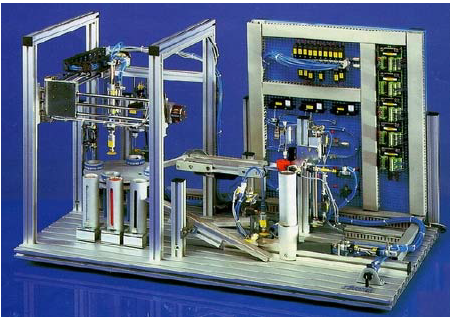
\includegraphics[scale=0.75]{FestoMPSSystem2.png}
					\caption{Το πλήρες σύστημα Festo MPS\textregistered}
					\label{φωτ:Το πλήρες σύστημα Festo MPS}
			\end{figure}
			
			\begin{figure}[hp]
					\centering
					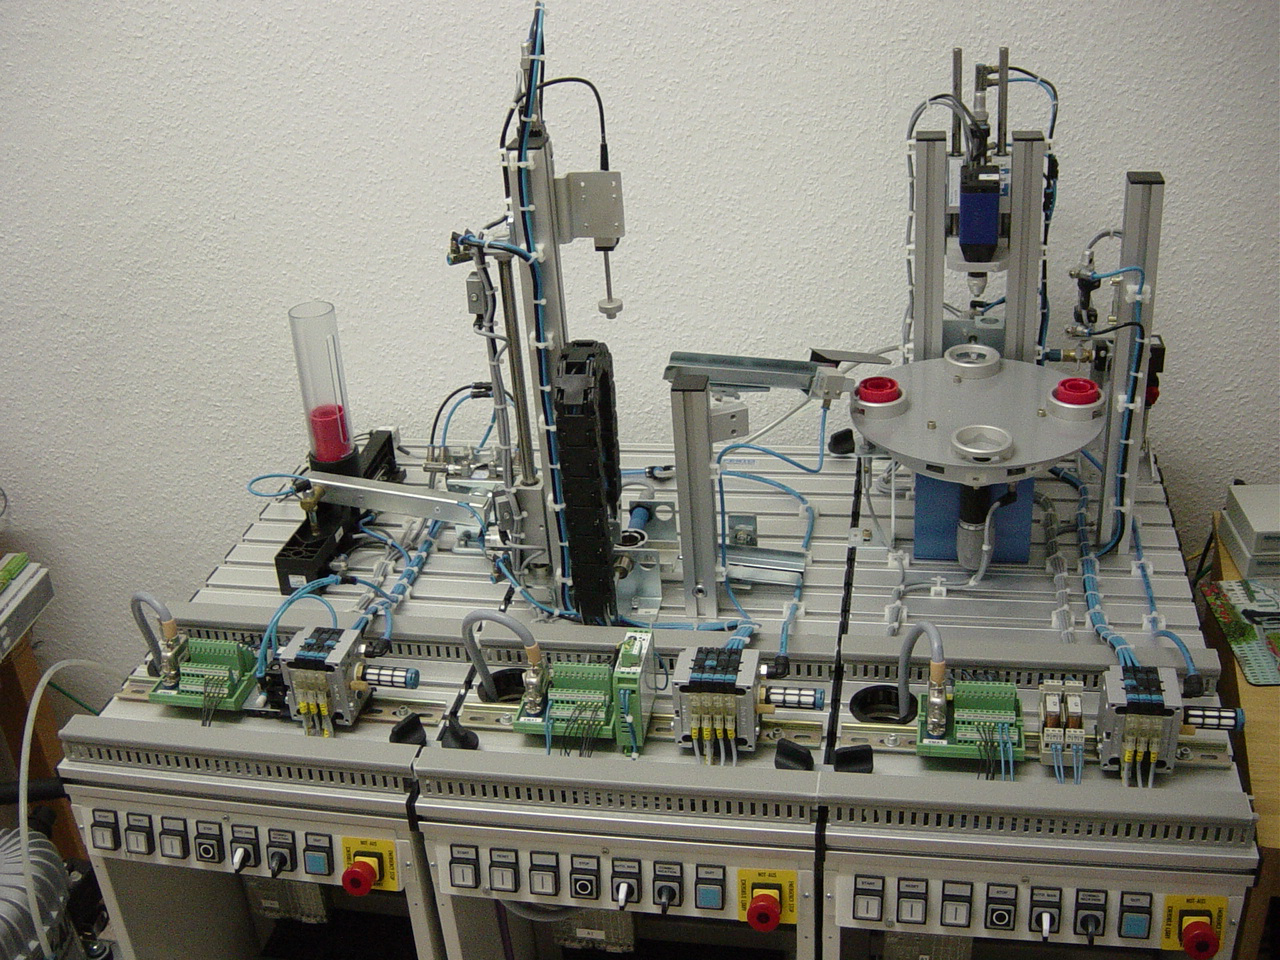
\includegraphics[scale=0.25]{FestoMPSSystem1.png}
					\caption{Το σύστημα Festo MPS\textregistered  χωρίς τον τελικό σταθμό αποθήκευσης \cite{PhotosFestoMPSUniversityHalle}}
					\label{φωτ:Το σύστημα Festo MPS χωρίς τον τελικό σταθμό αποθήκευσης}
			\end{figure}
			
			\paragraph{Κατασκευή} {Το σύστημα έχει κατασκευαστεί από την εταιρεία Festo Didactic\footnote{http://www.festo-didactic.com} \index{Festo Didactic}. Συγκεκριμένα η εταιρεία αυτή ειδικεύεται στη διδασκαλία συστημάτων αυτοματισμού. Για το σκοπό κατασκευάζει μικρογραφίες εξαρτημάτων όπως βαλβίδες πίεσης, κινητήρες, ρομποτικούς βραχίονες κ.ά. τα οποία συνδυαζώμενα μεταξύ τους αποδίδουν πληθώρα βιομηχανικών διεργασιών και συστημάτων παραγωγής. Ένα τέτοιο σύστημα αποτελεί και το συγκεκριμένο που θα αναλυθεί στη συνέχεια για τις ανάγκες της εργασίας.
			}
			
			\paragraph{Αιτιολόγηση επιλογής} {Επιλέξαμε το συγκεκριμένο σύστημα ως περίπτωση εφαρμογής για τη \acrshort{SysML} επειδή διαθέτει πολλά ενδιαφέροντα στοιχεία για έναν \glsuseriii{Μηχανικός συστημάτων} αφού αποτελείται από εξαρτήματα που ανήκουν σε διαφορετικά επιστημονικά πεδία. Συγκεκριμένα διαθέτει αισθητήρες που η αρχή λειτουργίας τους βασίζεται σε οπτική, επαγωγική, χωρητική και μηχανική μέτρηση. Επιπλέον περιλαμβάνει ηλεκτρικά, ηλεκτρονικά και μηχανικά μέρη, ρομποτικούς βραχίονες, βαλβίδες πίεσης, πνευματικές συσκευές κ.ά.. Μην ξεχνάμε ότι στο όλο σύστημα συμπεριλαμβάνεται και το λογισμικό ελέγχου της παραγωγικής διαδικασίας. Συνεπώς για την κατανόηση του απαιτούνται γνώσεις ηλεκτρολόγου, ηλεκτρονικού και μηχανολόγου μηχανικού καθώς και μηχανικού λογισμικού.
			}
						
			\paragraph{Πρώτες ύλες} {Ως πρώτες ύλες\index{πρώτη ύλη}\index{κυλινδρικά τεμάχια}\index{τεμάχια} χρησιμοποιούνται κυλινδρικά αντικείμενα διαφορετικού χρώματος, υλικού και ύψους. Μπορεί να είναι χρώματος κόκκινο, μαύρο ή ασημί και κατασκευασμένα από αλουμίνιο ή πλαστικό. Όσον αφορά το ύψος τους, τα κόκκινα και μεταλλικά τεμάχια είναι κατά 2,5 χιλιοστά ψηλότερα των αντίστοιχων μαύρων.
			}
			
			\begin{figure}[hp]
					\centering
					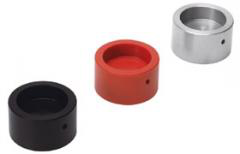
\includegraphics[scale=0.25]{WorkpiecesFesto.png}
					\caption{Οι πρώτες ύλες της γραμμής παραγωγής}
					\label{φωτ:Οι πρώτες ύλες της γραμμής παραγωγής}
			\end{figure}
		
			\paragraph{Παραγωγική διαδικασία} {Η παραγωγική διαδικασία που αναπαριστάμε έχει ως βάση της κυλινδρικά τεμάχια διάφορων χρωμάτων, υλικών και ύψους. Τα τεμάχια αυτά είναι αποθηκευμένα σε μία στοίβα στο σταθμό διανομής {\footnotesize (βλπ ενότ.~\ref{ενότ:Σταθμός διανομής})}. Με τη βοήθεια ενός βραχίονα μεταφέρονται στο σταθμό ελέγχου {\footnotesize (βλπ ενότ.~\ref{ενότ:Σταθμός ελέγχου})} όπου αναγνωρίζεται το χρώμα και το υλικό των κυλίνδρων και ελέγχονται για το ύψος τους. Αν κάποιος κύλινδρος διαθέτει μία ή και περισσότερες μη αποδεκτές ιδιότητες τότε απομακρύνεται από τη γραμμή παραγωγής. Οι αποδεκτοί πλέον κύλινδροι μεταβαίνουν στο σταθμό επεξεργασίας {\footnotesize (βλπ ενότ.~\ref{ενότ:Σταθμός επεξεργασίας})}. Στο σταθμό αυτό δημιουργείται μία οπή στο κέντρο των κυλίνδρων. Στη συνέχεια ελέγχεται αν η η διάτρηση ήταν επιτυχής και εν τέλει αποθηκεύονται στο σταθμό αποθήκευσης {\footnotesize (βλπ ενότ.~\ref{ενότ:Σταθμός αποθήκευσης})} σε μία από τρεις στοίβες ανάλογα με το χρώμα και το υλικό τους. \cite{UMLΕνσωματωμέναΣυστήματα}
			}
			
			\paragraph{} {Ακολουθεί η λειτουργική ανάλυση της κάθε μονάδας παραγωγής και η καταγραφή των επιμέρους μερών τους.}
			}

%%%%%%%%%%%%%%%%%%%%%%%%%%%%%%%%%%%%%%%%%%%%%%%%%%%%%%%%%%%%%
%%%%%%%%%%%%%%		   							Υποενότητα		   					   %%%%%%%%%%%%%%%%%%%%
			\FloatBarrier
			\subsection{Σταθμός διανομής \cite{FestoMPSDistributionStationManual} \cite{ΤοΦυσικόΣύστημαFestoMPS} \cite{UMLΕνσωματωμέναΣυστήματα}}
			
			\label{ενότ:Σταθμός διανομής}
				\paragraph{Εισαγωγή} {Ο σταθμός διανομής\index{σταθμός!διανομής} αναλαμβάνει την εισαγωγή των πρώτων υλών στη γραμμή παραγωγής από μία στοίβα αποθήκευσης\index{στοίβα αποθήκευσης} και τη διανομή τους με τη χρήση βραχίονα\index{βραχίονας} και βεντούζας\index{βεντούζα}. Αποτελείται από τα εξαρτήματα :
				}
				\begin{itemize}
					\item στοίβα αποθήκευσης {\footnotesize (βλπ. σχ.\ref{φωτ:Η στοίβα αποθήκευσης από Festo})}
					\item μονάδα μεταφοράς {\footnotesize (βλπ. σχ.\ref{φωτ:Η μονάδα μεταφοράς από Festo})}
					\item βάση εγκατάστασης
					\item συσκευή ελέγχου
					\item πλακέτα plc
				\end{itemize}
				\paragraph{} {Ο σταθμός διανομής διαχωρίζει τα κυλινδρικά τεμάχια από τη στοίβα αποθήκευσης η οποία διατηρεί μέχρι 8 κομμάτια. Το επίπεδο πλήρωσης της στοίβας ελέγχεται μέσω ενός \glsuseri{φωτοκύτταρο}. Οι κύλινδροι αφαιρούνται ένας-ένας από τη στοίβα μέσω ενός \glsuseri{έμβολο πεπιεσμένου αέρα δύο κατευθύνσεων}. Στη συνέχεια η \gls{μονάδα μεταφοράς} παραλαμβάνει τα τεμάχια και τα παραδίδει στον επόμενο σταθμό της γραμμής παραγωγής. Αυτό επιτυγχάνεται με τη χρήση ενός ρομποτικού βραχίονα και μιας \glsuseri{βεντούζα}. Η βεντούζα δεσμεύει το τεμάχιο με μία βαλβίδα κενού και ένας \gls{αισθητήρας κενού} ανιχνεύει τη δέσμευση του. Τότε ο βραχίονας μεταφοράς, οδηγούμενος από έναν κινητήρα περιστροφικής κίνησης, παραδίδει τον κύλινδρο στην επόμενη μονάδα.
				}
				
				\begin{figure}[hp]
					\centering
					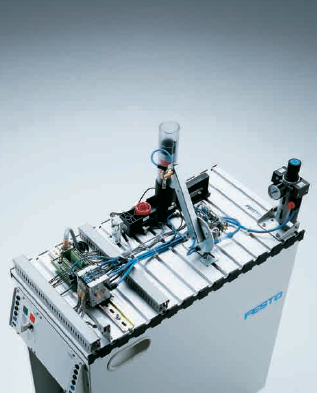
\includegraphics[scale=0.25]{DistributionStationFesto.png}
					\caption{Ο σταθμός διανομής \cite{OverviewMPSStations}}
					\label{φωτ:Ο σταθμός διανομής από Festo}
				\end{figure}
				
				\begin{figure}[hp]
					\centering
					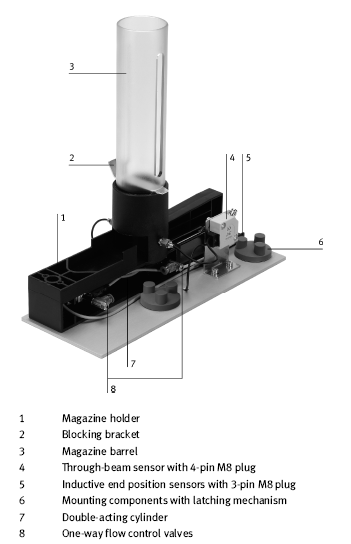
\includegraphics[scale=0.75]{StackModuleParts.png}
					\caption{Η στοίβα αποθήκευσης \cite{FestoStackMagazineModuleManual}}
					\label{φωτ:Η στοίβα αποθήκευσης από Festo}
				\end{figure}
				
				\begin{figure}[hp]
					\centering
					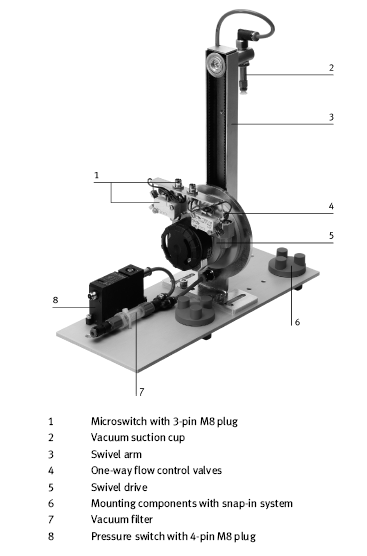
\includegraphics[scale=0.75]{ChangerModuleParts.png}
					\caption{Η μονάδα μεταφοράς \cite{FestoChangerModuleManual}}
					\label{φωτ:Η μονάδα μεταφοράς από Festo}
				\end{figure}
							

				
				\paragraph{Στοίβα αποθήκευσης {\footnotesize βλπ. σχ. \ref{φωτ:Η στοίβα αποθήκευσης από Θράμπο} και \ref{φωτ:Η στοίβα αποθήκευσης από Festo}}} {Όπως προαναφέρθηκε η στοίβα αποθήκευσης χωράει μέχρι 8 τεμάχια. Ένα πναυματικό έμβολο διπλής κατεύθυνσης μεταφέρει τα κομμάτια στην άκρη της μονάδας αυτής\index{έμβολο!διπλής κατεύθυνσης}. Τα τεμάχια σταματάνε στο σημείο αυτό επειδή υπάρχει κυκλικό τοιχίο που εμποδίζει οποιαδήποτε άλλη τοποθέτηση. Στη θέση αυτή χωράει μόνο ένα τεμάχιο και αποτελεί τη θέση από την οποία μεταφέρεται ο κύλινδρος στην επόμενη μονάδα.Το επόμενο τεμάχιο τοποθετείται αυτόματα μπροστά από το έμβολο με τη βοήθεια της βαρύτητας.
				}
				\paragraph{} {Η διαθεσιμότητα των τεμαχίων μέσα στη στοίβα διαπιστώνεται μέσω ενός φωτοκυττάρου\index{φωτοκύτταρο} τοποθετούμενο στο κάτω μέρος αυτής. Η θέση του εμβόλου διαπιστώνεται μαγνητικά μέσω δύο επαγωγικών αισθητήρων\index{επαγωγικός αισθητήρας}\index{αισθητήρας!επαγωγικός} -ο ένας αισθητήρας τοποθετείται στο πίσω μέρος και ο άλλος στο μπροστινό. Η ταχύτητα εκτόνωσης και επαναφοράς του εμβόλου καθορίζεται με μεγάλη ακρίβεια από \gls{βαλβίδα ελέγχου πεπιεσμένου αέρα μίας κατεύθυνσης}\index{βαλβίδα}.
				}

				\begin{figure}[hp]
					\centering
					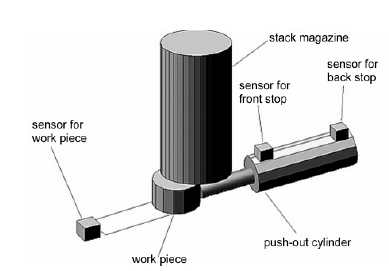
\includegraphics[scale=0.7]{StackModulePartsThrambo.png}
					\caption{Γραφική απεικόνιση της στοίβας αποθήκευσης \cite{ΤοΦυσικόΣύστημαFestoMPS}}
					\label{φωτ:Η στοίβα αποθήκευσης από Θράμπο}
				\end{figure}
	
				\paragraph{Μονάδα μεταφοράς {\footnotesize βλπ. σχ. \ref{φωτ:Η μονάδα μεταφοράς από Θράμπο} και \ref{φωτ:Η στοίβα αποθήκευσης από Festo}}} {\index{μονάδα!μεταφοράς}Η μονάδα αυτή αποτελεί μία πνευματική συσκευή. Μέσω μίας βεντούζας που είναι τοποθετημένη πάνω σε ρομποτικό βραχίονα τα τεμάχια μεταφέρονται με περιστροφική κίνηση\index{περιστροφική κίνηση} στην επόμενη μονάδα. Η περιστροφική κίνηση υλοποιείται από έναν πνευματικό κινητήρα\index{κινητήρας!πνευματικός}. Το εύρος της περιστροφικής κίνησης καθορίζεται μηχανικά μεταξύ 0 και 180 μοιρών. Οι τελικές θέσεις που λαμβάνει ο βραχίονας ελέγχονται μέσω \glsuserii{μικροδιακόπτης}\index{μικροδιακόπτης}. Τέλος μέσω ενός αισθητήρα κενού\index{αισθητήρας!κενού} συνδεδεμένο με τη βεντούζα ανιχνεύεται αν η τελευταία έχει παραλάβει το κυλινδρικό τεμάχιο.
				}
				\begin{figure}[hp]
					\centering
					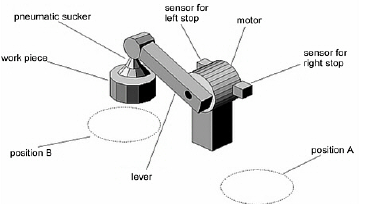
\includegraphics[scale=0.7]{ChangerModulePartsThrambo.png}
					\caption{Γραφική απεικόνιση της μονάδας μεταφοράς \cite{ΤοΦυσικόΣύστημαFestoMPS}}
					\label{φωτ:Η μονάδα μεταφοράς από Θράμπο}
				\end{figure}
				
				\paragraph{Ανάλυση λειτουργίας} {Λεπτομερέστερα οι προϋποθέσεις για να λειτουργήσει ο σταθμός αυτός και η σειρά με την οποία εκτελούνται οι επιμέρους ενέργειες απαριθμούνται στον πίνακα \ref{πιν.:Ανάλυση λειτουργίας του σταθμού διανομής}:
				}
				\begin{longtable} { m{0.5cm} m{12cm} }
					\caption [Ανάλυση λειτουργίας του σταθμού διανομής]  {Ανάλυση λειτουργίας του σταθμού διανομής \cite{FestoMPSDistributionStationManual}}
					\label{πιν.:Ανάλυση λειτουργίας του σταθμού διανομής}\\
					\hline
					\endfirsthead
					\multicolumn{2}{c}{συνέχεια του πίνακα \ref{πιν.:Ανάλυση λειτουργίας του σταθμού διανομής}}\\
					\hline
					~\\
					\endhead
					\hline
					\multicolumn{2}{c}{ο πίνακας συνεχίζεται στην επόμενη σελίδα}\\
					\endfoot
					\multicolumn{2}{c}{ολοκληρώθηκε ο πίνακας \ref{πιν.:Ανάλυση λειτουργίας του σταθμού διανομής}}\\
					\endlastfoot
					~\\
					\multicolumn{2}{c}{Προαπαιτήσεις}\\
					1 & Η στοίβα να διαθέτει τεμάχια προς επεξεργασία\\
					\hline
					~\\
					\multicolumn{2}{c}{Αρχική κατάσταση}\\
					1 & Το έμβολο διπλής κατεύθυνσης είναι σε κατάσταση εκτόνωσης\\
					2 & Το σύστημα βραχίονα-κινητήρα βρίσκεται στη μεριά της στοίβας\\
					3 & Η βεντούζα είναι ανενεργή\\
					\hline
					~\\
					\multicolumn{2}{c}{Ακολουθία ενεργειών}\\
					1 & Ο κινητήρας μεταβαίνει στη θέση του επόμενου σταθμού εάν υπάρχουν τεμάχια μέσα στη στοίβα και το πλήκτρο Εκκίνηση έχει πατηθεί\\
					2 & Το έμβολο επανέρχεται και βγάζει ένα τεμάχιο έξω από τη στοίβα\\
					3 & Ο κινητήρας μεταβαίνει στη θέση της στοίβας αποθήκευσης\\
					4 & Η βαλβίδα κενού ενεργοποιείται και μόλις πιαστεί το τεμάχιο ο διακόπτης κενού στέλνει το απαραίτητο σήμα\\
					5 & Το έμβολο επανέρχεται και ελευθερώνει το τεμάχιο\\
					6 & Ο κινητήρας μεταβαίνει στη θέση του επόμενου σταθμού\\
					7 & Η βαλβίδα κενού απενεργοποιείται\\
					8 & Ο κινητήρας μεταβαίνει στη θέση της στοίβας\\
					\hline
				\end{longtable}
			
%%%%%%%%%%%%%%%%%%%%%%%%%%%%%%%%%%%%%%%%%%%%%%%%%%%%%%%%%%%%%
%%%%%%%%%%%%%%		   							Υποενότητα		   					   %%%%%%%%%%%%%%%%%%%%
			\FloatBarrier
			\subsection{Σταθμός ελέγχου \cite{FestoMPSTestingStationManual} \cite{ΤοΦυσικόΣύστημαFestoMPS} \cite{UMLΕνσωματωμέναΣυστήματα}}
			
			\label{ενότ:Σταθμός ελέγχου}
				\paragraph{Εισαγωγή} {Ο σταθμός ελέγχου\index{σταθμός!ελέγχου} αναλαμβάνει να διαπιστώσει αν το τεμάχιο που παρέλαβε από το σταθμό διανομής {\footnotesize βλπ. ενοτ.\ref{ενότ:Σταθμός διανομής}} είναι κατάλληλο επεξεργασίας από τον επόμενο σταθμό -σταθμός επεξεργασίας {\footnotesize βλπ. ενοτ.\ref{ενότ:Σταθμός επεξεργασίας}}. Συγκεκριμένα πρέπει να αναγνωρίσει το υλικό κατασκευής των κυλίνδρων, να ελέγξει το ύψος των τεμαχίων και ανάλογα με αυτό να τον απορρίψει  ή να τον προωθήσει στον επόμενο σταθμό της γραμμής παραγωγής. Αποτελείται από τα εξαρτήματα :
				}
				\begin{itemize}
					\item μονάδα αναγνώρισης
					\item μονάδα ανύψωσης
					\item μονάδα μέτρησης
					\item μονάδα κύλισης με αέρα
					\item μονάδα κύλισης
					\item βάση εγκατάστασης
					\item συσκευή ελέγχου
					\item πλακέτα plc
				\end{itemize}
				\paragraph{} {Ο σταθμός ελέγχου εξακριβώνει τα χαρακτηριστικά των κυλινδρικών τεμαχίων. Η μονάδα αναγνώρισης διαπιστώνει το χρώμα του κυλίνδρου και την παρουσία τεμαχίου. Με \glsuseri{αισθητήρας ανάκλασης}\index{αισθητήρας!ανάκλασης} ελέγχουμε αν η θέση μέτρησης είναι διαθέσιμη ώστε να αποφασιστεί αν θα ανυψωθεί το κυλινδρικό αντικείμενο ή όχι. Επιπλέον, ένας \gls{αναλογικός αισθητήρας}\index{αισθητήρας!αναλογικός} μετράει το ύψος του κυλίνδρου. Το σήμα εξόδου του αισθητήρα μετατρέπεται σε ψηφιακό μέσω ενός τελεστή με ρυθμιζόμενο κατώφλι ή μπορεί να εισαχθεί σε ένα PLC ως αναλογικό σήμα. Τέλος αν οι κύλινδροι είναι αποδεκτοί οδηγούνται από το επίπεδο που είναι με ένα πνευματικό \gls{γραμμικό έμβολο}\index{έμβολο!γραμμικό} δύο κατευθύνσεων προς τον σταθμό επεξεργασίας διαμέσου μιας \glsuseri{πλατφόρμα κύλισης με εξομάλυνση αέρα}\index{πλατφόρμα κύλισης!εξομάλυνση αέρα}. Τα υπόλοιπα κομμάτια "κατεβαίνουν" πίσω με τον ανελκυστήρα και τοποθετούνται σε μία διπλανή \gls{πλατφόρμα κύλισης}.
				}
				
				\begin{figure}[hp]
					\centering
					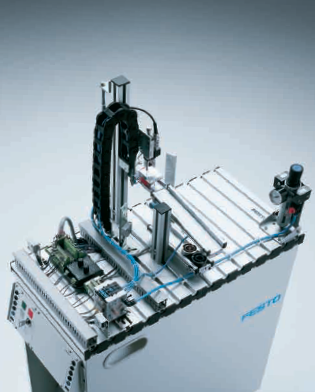
\includegraphics[scale=0.25]{TestingStationFesto.png}
					\caption{Ο σταθμός ελέγχου \cite{OverviewMPSStations}}
					\label{φωτ:Ο σταθμός ελέγχου από Festo}
				\end{figure}
								
				\paragraph{Μονάδα αναγνώρισης {\footnotesize βλπ. σχ. \ref{φωτ:Η μονάδα αναγνώρισης από Festo}}\index{μονάδα!αναγνώρισης}} {Η μονάδα αυτή αποτελείται από 2 \glsplural{αισθητήρας προσέγγισης}\index{αισθητήρας!προσέγγισης} με ψηφιακή έξοδο, έναν χωρητικό και έναν οπτικό\index{αισθητήρας!οπτικός}. Ο χωρητικός ανιχνεύει την παρουσία τεμαχίου ανεξαρτήτως χρώματος. Αντίστοιχα ο οπτικός αισθητήρας διάχυσης ανιχνεύει το χρώμα των αντικειμένων. Επειδή η αρχή λειτουργίας του βασίζεται στην ποσότητα του επιστρεφόμενου φωτός, δεν μπορούν να ανιχνευθούν τα μαύρα τεμάχια. Ο οπτικός αισθητήρας τοποθετείται πάνω στην πλατφόρμα ανύψωσης.
				}
				\begin{figure}[hp]
					\centering
					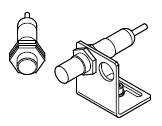
\includegraphics[scale=1]{TestingStationRecognitionModule.png}
					\caption{Η μονάδα αναγνώρισης \cite{FestoMPSTestingStationManual}}
					\label{φωτ:Η μονάδα αναγνώρισης από Festo}
				\end{figure}
				
				\paragraph{Μονάδα ανύψωσης {\footnotesize βλπ. σχ. \ref{φωτ:Η μονάδα ανύψωσης από Festo}}\index{μονάδα!ανύψωσης}} {Η ανύψωση πραγματοποιείται με ένα \gls{πνευματικό έμβολο}\index{έμβολο!πνευματικό} δύο κατευθύνσεων. Η χαμηλή και ψηλή θέση του εντοπίζονται μέσω \glsuserii{μαγνητικός αισθητήρας}\index{αισθητήρας!μαγνητικός} ή \glsuserii{επαγωγικός αισθητήρας}\index{αισθητήρας!επαγωγικός}. Επιπλέον, διαθέτει ένα πνευματικό \gls{έμβολο εκτίναξης}\index{έμβολο!εκτίναξης} δύο κατευθύνσεων για την απομάκρυνση των αποδεκτών τεμαχίων στην μονάδα κύλισης με εξομάλυνση αέρα και των απορριφθέντων τεμαχίων στην απλή μονάδα κύλισης. Η θέση του εμβόλου αυτού διαπιστώνεται μέσω δύο μαγνητικών αισθητήρων, έναν στο μπροστινό τμήμα του και ένα στο πίσω. Τέλος, για την καλύτερη και ασφαλέστερη εγκατάσταση των εξαρτημάτων αυτών χρησιμοποιείται και ένας οδηγός τύπου αλυσίδας για ενθυλακώσει τα ηλεκτρικά καλώδια και τους σωλήνες μεταφοράς πεπιεσμένου αέρα της διάταξης. Επισημαίνουμε ότι ο οπτικός αισθητήρας της μονάδας αναγνώρισης ενσωματώνεται πάνω στην πλατφόρμα ανύψωσης.
				}
				\begin{figure}[hp]
					\centering
					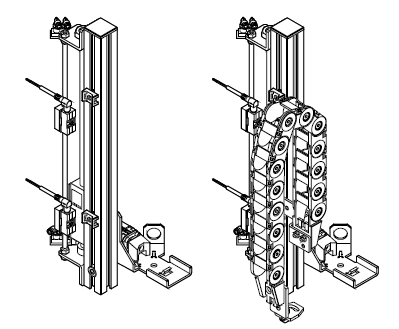
\includegraphics[scale=0.5]{TestingStationLiftingModule.png}
					\caption{Η μονάδα ανύψωσης \cite{FestoMPSTestingStationManual} (στη δεύτερη εικόνα εμφανίζεται ο οδηγός καλωδίων στον οποίο τοποθετούνται τα ηλεκτρικά καλώδια και οι σωλήνες μεταφοράς πεπιεσμένου αέρα)}
					\label{φωτ:Η μονάδα ανύψωσης από Festo}
				\end{figure}
				
				\paragraph{Μονάδα μέτρησης {\footnotesize βλπ. σχ. \ref{φωτ:Η μονάδα μέτρησης από Festo} και \ref{φωτ:Σχηματική απεικόνιση της μονάδας μέτρησης από Θράμπο}}\index{μονάδα!μέτρησης}} {Αποτελείται από ένα αναλογικό αισθητήρα για τη μέτρηση του ύψους των τεμαχίων. Η αρχή λειτουργίας βασίζεται σε έναν γραμμικό ποτενσιόμετρο και ένα διαιρέτη τάσης. Η αναλογική μέτρηση μπορεί να μετατραπεί σε ψηφιακή μέσω ενός τελεστή ή να τροφοδοτηθεί σε μία plc συσκευή. Τέλος υπάρχει αποσβέστης ταλαντώσεων που δημιουργούνται από την ανύψωση του αντικειμένου στην τελική του θέση.\\Επισημαίνουμε ότι τα κόκκινα και μεταλλικά τεμάχια είναι κατά 2,5 χιλιοστά ψηλότερα των αντίστοιχων μαύρων.
				}
				\begin{figure}[hp]
					\centering
					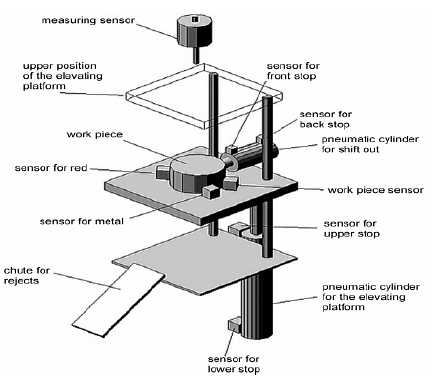
\includegraphics[scale=1]{TestingStationPartsThrambo.png}
					\caption{Σχηματική απεικόνιση της μονάδας μέτρησης \cite{ΤοΦυσικόΣύστημαFestoMPS}}
					\label{φωτ:Σχηματική απεικόνιση της μονάδας μέτρησης από Θράμπο}
				\end{figure}	
				
				\begin{figure}[hp]
					\centering
					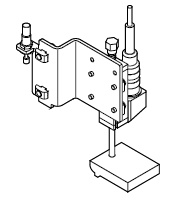
\includegraphics[scale=1]{TestingStationMeasuringModule.png}
					\caption{Η μονάδα μέτρησης \cite{FestoMPSTestingStationManual}}
					\label{φωτ:Η μονάδα μέτρησης από Festo}
				\end{figure}			
				
				\paragraph{Μονάδα κύλισης με εξομάλυνση αέρα {\footnotesize βλπ. σχ. \ref{φωτ:Η μονάδα κύλισης με εξομάλυνση αέρα από Festo} και \ref{φωτ:Σχηματική απεικόνιση της μονάδας κύλισης με εξομάλυνση αέρα από Θράμπο}}\index{μονάδα!κύλισης με εξομάλυνση αέρα}} {Η μονάδα κύλισης με εξομάλυνση αέρα χρησιμοποιείται για τη μεταφορά των κυλίνδρων με μέγιστη χωρητικότητα πέντε (5). Η εξομάλυνση από τον αέρα μειώνει την τριβή μεταξύ των τεμαχίων και της πλατφόρμας. Η γωνία κλίσης της πλατφόρμας είναι ρυθμιζόμενη. Στο τέλος της πλατφόρμας δεν υπάρχει τοιχίο για να εμποδίζει την κύλιση των κυλίνδρων. Επιθυμούμε την απρόσκοπτη κύλιση τους στον επόμενο σταθμό.
				}
				\begin{figure}[hp]
					\centering
					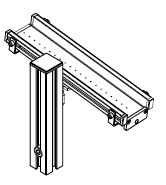
\includegraphics[scale=1]{TestingStationAirCushionedSlideModule.png}
					\caption{Η μονάδα κύλισης με εξομάλυνση αέρα \cite{FestoMPSTestingStationManual}}
					\label{φωτ:Η μονάδα κύλισης με εξομάλυνση αέρα από Festo}
				\end{figure}
				\begin{figure}[hp]
					\centering
					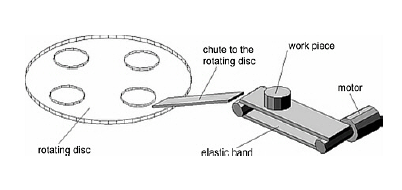
\includegraphics[scale=1]{TestingStationAirCushionedSlideTrambo.png}
					\caption{Σχηματική απεικόνιση της μονάδας κύλισης με εξομάλυνση αέρα \cite{ΤοΦυσικόΣύστημαFestoMPS}}
					\label{φωτ:Σχηματική απεικόνιση της μονάδας κύλισης με εξομάλυνση αέρα από Θράμπο}
				\end{figure}
				
				\paragraph{Μονάδα κύλισης {\footnotesize βλπ. σχ. \ref{φωτ:Η μονάδα κύλισης από Festo}} \index{μονάδα!κύλισης}} {Η μονάδα κύλισης χρησιμοποιείται για τη μεταφορά των κυλίνδρων. Τέσσερα (4) στο σύνολο μπορούν να τοποθετηθούν στην πλατφόρμα. Η γωνία κλίσης είναι ρυθμιζόμενη.
				}
				\begin{figure}[hp]
					\centering
					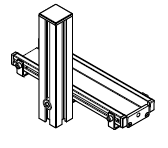
\includegraphics[scale=1]{TestingStationSlideModule.png}
					\caption{Η μονάδα κύλισης \cite{FestoMPSTestingStationManual}}
					\label{φωτ:Η μονάδα κύλισης από Festo}
				\end{figure}
				
				
				\paragraph{Ανάλυση λειτουργίας} {Λεπτομερέστερα οι προϋποθέσεις για να λειτουργήσει ο σταθμός αυτός και η σειρά με την οποία εκτελούνται οι επιμέρους ενέργειες απαριθμούνται στον πίνακα \ref{πιν.:Ανάλυση λειτουργίας του σταθμού ελέγχου}:
				}
				\begin{longtable} { m{0.5cm} m{12cm} }
					\caption [Ανάλυση λειτουργίας του σταθμού ελέγχου]  {Ανάλυση λειτουργίας του σταθμού ελέγχου \cite{FestoMPSTestingStationManual}}
					\label{πιν.:Ανάλυση λειτουργίας του σταθμού ελέγχου}\\
					\hline
					\endfirsthead
					\multicolumn{2}{c}{συνέχεια του πίνακα \ref{πιν.:Ανάλυση λειτουργίας του σταθμού ελέγχου}}\\
					\hline
					~\\
					\endhead
					\hline
					\multicolumn{2}{c}{ο πίνακας συνεχίζεται στην επόμενη σελίδα}\\
					\endfoot
					\multicolumn{2}{c}{ολοκληρώθηκε ο πίνακας \ref{πιν.:Ανάλυση λειτουργίας του σταθμού ελέγχου}}\\
					\endlastfoot
					~\\
					\multicolumn{2}{c}{Προαπαιτήσεις}\\
					1 & Ένα τεμάχιο βρίσκεται έτοιμο για παραλαβή στο σταθμό διανομής\\
					2 & Κανένα άλλο τεμάχιο δεν καταλαμβάνει την θέση αναγνώρισης\\
					\hline
					~\\
					\multicolumn{2}{c}{Αρχική κατάσταση}\\
					1 & Ο ανελκυστήρας μεταβαίνει στην χαμηλή θέση\\
					2 & Το έμβολο εκτίναξης συμπτύσσεται\\
					3 & Απενεργοποίηση της πλατφόρμας κύλισης με εξομάλυνση αέρα\\
					\hline
					~\\
					\multicolumn{2}{c}{Ακολουθία ενεργειών}\\
					1 & Αναγνώριση χρώματος και υλικού των τεμαχίων\\
					2 & Ο ανελκυστήρας ανέρχεται στην πάνω θέση\\
					3 & Γίνεται έλεγχος του ύψους\\
					   & Αποδεκτό κυλινδρικό τεμάχιο\\
					 4 & Ενεργοποίηση της πλατφόρμας κύλισης με εξομάλυνση αέρα\\
					 5 & Έκταση του εμβόλου εκτίναξης\\
					 6 & Σύμπτυξη του εμβόλου εκτίναξης\\
					 7 & Απενεργοποίηση της πλατφόρμας κύλισης με εξομάλυνση αέρα\\
					 8 & Ο ανελκυστήρας κατέρχεται στην χαμηλή θέση\\
					 9 & Αρχική θέση\\
					  & Μη αποδεκτό κυλινδρικό τεμάχιο\\
					 10 & Ο ανελκυστήρας κατέρχεται στην χαμηλή θέση\\
					 11 & Έκταση του εμβόλου εκτίναξης\\
					 12 & Σύμπτυξη του εμβόλου εκτίναξης\\
					 13 & Αρχική θέση\\
					\hline
				\end{longtable}
				
				
%%%%%%%%%%%%%%%%%%%%%%%%%%%%%%%%%%%%%%%%%%%%%%%%%%%%%%%%%%%%%
%%%%%%%%%%%%%%		   							Υποενότητα		   					   %%%%%%%%%%%%%%%%%%%%			
			\FloatBarrier
			\subsection{Σταθμός επεξεργασίας \cite{FestoMPSProcessingStationManual} \cite{ΤοΦυσικόΣύστημαFestoMPS} \cite{UMLΕνσωματωμέναΣυστήματα}}
			
			\label{ενότ:Σταθμός επεξεργασίας}
				\paragraph{Εισαγωγή} {Ο σταθμός επεξεργασίας\index{σταθμός!επεξεργασίας} αναλαμβάνει να επεξεργαστεί τα κυλινδρικά τεμάχια. Συγκεκριμένα πρέπει να τους επιφέρει μία οπή στο πάνω μέρος τους. Αποτελείται από τα εξαρτήματα :
				}
				\begin{itemize}
					\item μονάδα περιστροφής
					\item μονάδα διάτρησης
					\item μονάδα ελέγχου
					\item βάση εγκατάστασης
					\item συσκευή ελέγχου
					\item πλακέτα plc
				\end{itemize}
				\paragraph{} {Ο σταθμός αυτός διαθέτει ένα περιστρεφόμενο δίσκο με τέσσερις (4) θέσεις για τα κυλινδρικά τεμάχια. Η θέση του δίσκου διαπιστώνεται με έναν επαγωγικό αισθητήρα, ο οποίος ανιχνεύει μεταλλική βίδα που υπάρχει σε κάθε μία από τις τέσσερις θέσεις. Αρχικά εισέρχεται κύλινδρος προς επεξεργασία. Ο δίσκος περιστρέφεται κατά $90^{\circ}$ στη θέση όπου βρίσκεται το τρυπάνι. Στη θέση αυτή το τεμάχιο ακινητοποιείται με τη βοήθεια ενός ηλεκτρομαγνητικού εμβόλου δύο κατευθύνσεων. Στη συνέχεια το τρυπάνι επιφέρει μία οπή στο τεμάχιο. Έπειτα ο δίσκος περιστρέφεται άλλες $90^{\circ}$. Στη θέση αυτή ελέγχεται αν η οπή είναι αποδεκτή. Ο έλεγχος γίνεται με μία ακίδα η οποία κινείται με μία ηλεκτρομαγνητική διάταξη. Τέλος, ο δίσκος περιστρέφεται κατά $90^{\circ}$ αναμένοντας το σταθμό αποθήκευσης να παραλάβει το επεξεργασμένο πλέον τεμάχιο.
				}
				\paragraph{} {Οι δύο διεργασίες του σταθμού αυτού -η διάτρηση και ο έλεγχος της οπής- γίνονται παράλληλα. Στον περιστερφόμενο δίσκο δεν εισέρχεται ένα τεμάχιο, επεξεργάζεται, ελέγχεται και μεταβαίνει στη μονάδα αποθήκευσης και έπειτα ένα δεύτερο. Αντίθετα, μπορεί και οι τέσσερις θέσεις να είναι κατειλημμένες ταυτόχρονα από κυλινδρικά τεμάχια. Φυσικά κάθε τεμάχιο θα συμμετέχει και σε διαφορετική διεργασία.
				}
				\begin{figure}[hp]
					\centering
					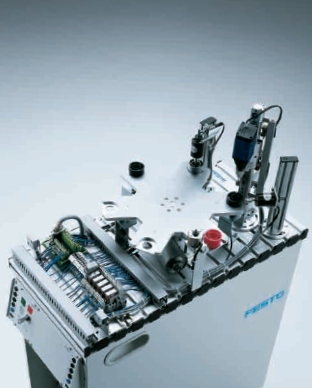
\includegraphics[scale=0.25]{ProcessingStationFesto.png}
					\caption{Ο σταθμός επεξεργασίας \cite{OverviewMPSStations}}
					\label{φωτ:Ο σταθμός επεξεργασίας από Festo}
				\end{figure}
								
				\paragraph{Μονάδα περιστροφής\index{μονάδα!περιστροφής}} {Η μονάδα αυτή ελέγχεται από μία \gls{μηχανή γραναζωτής σύμπλεξης συνεχούς ρεύματος}\index{μηχανή!συνεχούς ρεύματος}. Διαθέτει τέσσερις (4) θέσεις για να τις καταλάβουν τα τεμάχια. Σε κάθε θέση υπάρχει ένας χωρητικός αισθητήρας προσέγγισης για να διευκρινίζεται αν η θέση είναι πλήροις ή όχι.
				}
				
				\paragraph{Μονάδα διάτρησης {\footnotesize (βλπ. σχ. \ref{φωτ:Η μονάδα διάτρησης από Festo} και \ref{φωτ:Σχηματική αναπαράσταση της μονάδας διάτρησης από Θράμπο})}\index{μονάδα!διάτρησης}} {Στη θέση αυτή όταν διαπιστωθεί η ύπαρξη τεμαχίου ενεργοποιείται ένα πνευματικό έμβολο\index{έμβολο!ηλεκτρικό} δύο κατευθύνσεων για να το συγκρατήσει ακίνητο. Για τη καταγραφή της θέσης του εμβόλουχρησιμοποιούνται και πάλι δύο μαγνητικοί αισθητήρες, ένας μπροστά και ο δεύτερος στο πίσω μέρος. Στη συνέχεια το τρυπάνι\index{τρυπάνι} τρυπάει το τεμάχιο αυτό. Το τρυπάνι κινείται με τη βοήθεια ενός κινητήρα και η σύμπλεξη κινητήρα-τρυπανιού γίνεται μέσω οδοντωτού ιμάντα\index{οδοντωτός ιμάντας}\index{ιμάντας}. Η θέση του τρυπανιού ρυθμίζεται από δύο (2) ηλεκτρικούς τερματικούς διακόπτες\index{διακόπτης!ηλεκτρικός}\index{διακόπτης!τερματικός} που βρίσκονται στις δύο ακραίες θέσεις του τρυπανιού. Κάθε φορά που το σώμα από το τρυπάνι πλησιάζει έναν από τους δύο τερματικούς διακόπτες η κίνησή του αντιστρέφεται. Δηλαδή άμα κατέρχεται αλλάζει φορά και ανέρχεται και αντίστροφα. Υπενθυμίζεται ότι στη θέση αυτή υπάρχει χωρητικός αισθητήρας για να εξακριβωθεί ότι η θέση είναι κατειλημμένη.
				}
				\begin{figure}[hp]
					\centering
					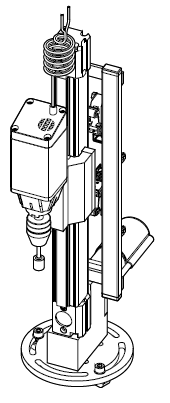
\includegraphics[scale=1]{ProcessingStationDrillingModuleFesto.png}
					\caption{Η μονάδα διάτρησης \cite{FestoMPSProcessingStationManual}}
					\label{φωτ:Η μονάδα διάτρησης από Festo}
				\end{figure}
				
				\begin{figure}[hp]
					\centering
					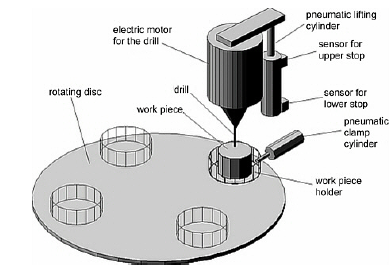
\includegraphics[scale=0.75]{ProcessingStationDrillingModuleThrambo.png}
					\caption{Σχηματική αναπαράσταση της μονάδας διάτρησης \cite{ΤοΦυσικόΣύστημαFestoMPS} {\footnotesize Παρατηρείται ότι το τρυπάνι κινείται με τη βοήθεια πνευματικού κυλίνδρου και όχι με ηλεκτρικό κινητήρα όπως αναφέρεται στο κείμενο. Καταγράψαμε την διάταξη όπως αυτή τεκμηριώνεται στο \cite{FestoMPSProcessingStationManual}. Η εικόνα παρατίθεται μόνο για να βοηθήσει να οπτικοποιηθεί το εν λόγω σύστημα}}
					\label{φωτ:Σχηματική αναπαράσταση της μονάδας διάτρησης από Θράμπο}
				\end{figure}
				
				\paragraph{Μονάδα ελέγχου {\footnotesize (βλπ. σχ. \ref{φωτ:Η μονάδα ελέγχου από Festo} και \ref{φωτ:Σχηματική αναπαράσταση της μονάδας ελέγχου από Θράμπο})}\index{μονάδα!ελέγχου}} {Η μονάδα ελέγχου αποτελεί μία \gls{ηλεκτρομαγνητική διάταξη}\index{ηλεκτρομαγνητική διάταξη}. Υπάρχει ένα πηνίο το οποίο παραμένει πακτωμένο στο πάνω μέρος του κορμού στήριξης. Όταν το πηνίο διαρρέεται από ρεύμα τότε, ο οπλισμός κατέρχεται και συνεπώς η ακίδα ελέγχου προσεγγίζει το επίπεδο του περιστρεφόμενου δίσκου, το επίπεδο δηλαδή του προς εξέταση κυλίνδρου. Για την διαπίστωση της θέσης του συστήματος ακίδας-οπλισμού χρησιμοποιούνται δύο επαγωγικοί αισθητήρες προσέγγισης\index{αισθητήρας!επαγωγικός}\index{αισθητήρας!προσέγγισης} οι οποίοι ενεργοποιούνται μέσω ενός μεταλλικού παξιμαδιού βρισκόμενο στο πάνω μέρος του συστήματος ακίδας-οπλισμού. Για τη διαπίστωση της ορθότηταας της τρύπας, η ακίδα της διάταξης αποτελεί ένα επαγωγικός αισθητήρας προσέγγισης.  Υπενθυμίζεται ότι στη θέση αυτή υπάρχει χωρητικός αισθητήρας για να εξακριβωθεί ότι η θέση είναι κατειλημμένη.
				}
				\begin{figure}[hp]
					\centering
					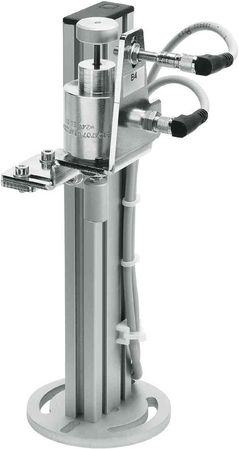
\includegraphics[scale=0.5]{ProcessingStationTestingModuleFesto.png}
					\caption{Η μονάδα ελέγχου {\footnotesize http://www.festo-didactic.com/int-en/learning-systems/mps-the-modular-production-system/project-kits/components-modules/testing-module.htm?fbid=aW50LmVuLjU1Ny4xNy4xOC43MTAuMzk0MQ}}
					\label{φωτ:Η μονάδα ελέγχου από Festo}
				\end{figure}
				
				\begin{figure}[hp]
					\centering
					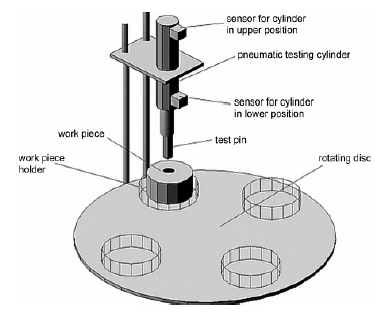
\includegraphics[scale=0.75]{ProcessingStationTestingModuleTrambo.png}
					\caption{Σχηματική αναπαράσταση της μονάδας ελέγχου \cite{ΤοΦυσικόΣύστημαFestoMPS} {\footnotesize Παρατηρείται ότι η ακίδα κινείται με τη βοήθεια πνευματικού κυλίνδρου και όχι με ηλεκτρομαγνητική διάταξη όπως αναφέρεται στο κείμενο. Καταγράψαμε την διάταξη όπως αυτή τεκμηριώνεται στο \cite{FestoMPSProcessingStationManual}. Η εικόνα παρατίθεται μόνο για να βοηθήσει να οπτικοποιηθεί το εν λόγω σύστημα}}
					\label{φωτ:Σχηματική αναπαράσταση της μονάδας ελέγχου από Θράμπο}
				\end{figure}			
				
				\paragraph{Ανάλυση λειτουργίας} {Λεπτομερέστερα οι προϋποθέσεις για να λειτουργήσει ο σταθμός αυτός και η σειρά με την οποία εκτελούνται οι επιμέρους ενέργειες απαριθμούνται στον πίνακα \ref{πιν.:Ανάλυση λειτουργίας του σταθμού επεξεργασίας}:
				}
				\begin{longtable} { m{0.5cm} m{12cm} }
					\caption [Ανάλυση λειτουργίας του σταθμού επεξεργασίας]  {Ανάλυση λειτουργίας του σταθμού επεξεργασίας \cite{FestoMPSProcessingStationManual}}
					\label{πιν.:Ανάλυση λειτουργίας του σταθμού επεξεργασίας}\\
					\hline
					\endfirsthead
					\multicolumn{2}{c}{συνέχεια του πίνακα \ref{πιν.:Ανάλυση λειτουργίας του σταθμού επεξεργασίας}}\\
					\hline
					\endhead
					\hline
					\multicolumn{2}{c}{ο πίνακας συνεχίζεται στην επόμενη σελίδα}\\
					\endfoot
					\multicolumn{2}{c}{ολοκληρώθηκε ο πίνακας \ref{πιν.:Ανάλυση λειτουργίας του σταθμού επεξεργασίας}}\\
					\endlastfoot
					~\\
					\multicolumn{2}{c}{Προαπαιτήσεις}\\
					1 & Κυλινδρικό τεμάχιο υπάρχει στην θέση υποδοχής του περιστρεφόμενου δίσκου\\
					\hline
					~\\
					\multicolumn{2}{c}{Αρχική κατάσταση}\\
					1 & Διαπιστώνεται η θέση του δίσκου\\
					2 & Η ακίδα ελέγχου βρίσκεται στην υψηλότερη θέση.\\
					3 & Το τρυπάνι διάτρησης βρίσκεται στην υψηλότερη θέση.\\
					4 & Το τρυπάνι είναι απενεργοποιημένο.\\
					5 & Το έμβολο συγκράτησης των κυλίνδρων στη θέση διάτρησης είναι σε κατάσταση σύμπτυξης.\\
					\hline
					~\\
					\multicolumn{2}{c}{Ακολουθία ενεργειών}\\
					  & Η ακολουθία αυτή αναφέρεται στην περίπτωση που ένα μόνο τεμάχιο βρίσκεται σε όλο τον περιστρεφόμενο δίσκο.\\
					1 & Ο δίσκος περιστρέφεται κατά $90^{\circ}$ εάν ανιχνευθεί τεμάχιο στη θέση υποδοχής. και το πλήκτρο εκκίνησης έχει πατηθεί.\\
					2 & Το έμβολο συγκράτησης εκτείνεται αφού πλέον το τεμάχιο βρίσκεται στη θέση διάτρησης. Το τρυπάνι ενεργοποιείται και κατέρχεται.\\
					3 & Μόλις το τρυπάνι φτάσει την κατώτατη θέση του, αυτόματα επανέρχεται στην ανώτερή του θέση.\\
					4 & Το τρυπάνι απενεργοποιείται και το έμβολο συγκράτησης συμπτύσεται.\\
					5 & Ο δίσκος περιστρέφεται κατά $90^{\circ}$.\\
					6 & Η ακίδα ελέγχου κατέρχεται και ελέγχει αν η οπή είναι η επιθυμητή.\\
					7 & Ο δίσκος περιστρέφεται κατά $90^{\circ}$ με αποτέλεσμα το τεμάχιο να μεταβεί στη θέση παραλαβής του από τον επόμενο σταθμό.\\
					\hline
				\end{longtable}

%%%%%%%%%%%%%%%%%%%%%%%%%%%%%%%%%%%%%%%%%%%%%%%%%%%%%%%%%%%%%
%%%%%%%%%%%%%%		   							Υποενότητα		   					   %%%%%%%%%%%%%%%%%%%%			
			\FloatBarrier
			\subsection{Σταθμός αποθήκευσης \cite{FestoMPSHandlingStationManual} \cite{ΤοΦυσικόΣύστημαFestoMPS} \cite{UMLΕνσωματωμέναΣυστήματα}}
			
			\label{ενότ:Σταθμός αποθήκευσης}
				\paragraph{Εισαγωγή} {Ο σταθμός αποθήκευσης\index{σταθμός!αποθήκευσης} αναλαμβάνει να μεταφέρει τα κυλινδρικά τεμάχια από τον περιστρεφόμενο δίσκο στις στοίβες αποθήκευσης. Αποτελείται από τα εξαρτήματα :
				}
				\begin{itemize}
					\item μονάδα μεταφοράς
					\item μονάδα αποθήκευσης
					\item βάση εγκατάστασης
					\item συσκευή ελέγχου
					\item πλακέτα plc
				\end{itemize}
				\paragraph{} {Το κυλινδρικό τεμάχιο το οποίο είναι έτοιμο για αποθήκευση παραλαμβάνεται από μία δαγκάνα με πνευματική αρχή λειτουργίας που κινείται με ένα σύστημα μεταφοράς δύο αξόνων. Ανάλογα με το είδος του κυλίνδρου και το γεγονός ότι η διάτρηση ήταν επιτυχής ή όχι, οι κύλινδροι μεταφέρονται σε τρεις (3) στοίβες. Αν το τεμάχιο είναι μαύρο τότε αποθηκεύεται στην πρώτη (εσωτερική) στοίβα. Αν το αντικείμενο είναι κόκκινου ή ασημί χρώματος τότε εναποτίθεται στην δεύτερη (μεσαία) στοίβα. Τέλος, αν η οπή δεν ειναι η επιθυμητή τότε μεταφέρεται στην τρίκη (εξωτερική) στοίβα.
				}
				\begin{figure}[hp]
					\centering
					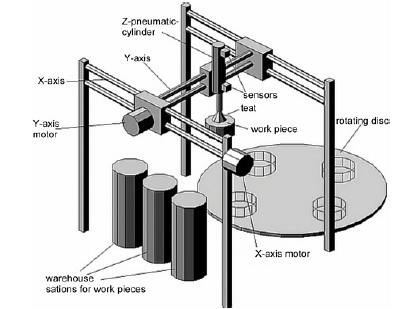
\includegraphics[scale=0.75]{HandlingStationTrambo.png}
					\caption{Ο σταθμός αποθήκευσης \cite{ΤοΦυσικόΣύστημαFestoMPS}  {\footnotesize Παρατηρείται ότι η διάταξη μεταφοράς περιλαμβάνει βεντούζα και όχι δαγκάνα όπως αναφέρεται στο κείμενο. Καταγράψαμε την διάταξη ως συνδυασμό των \cite{FestoMPSHandlingStationManual} και \cite{ΤοΦυσικόΣύστημαFestoMPS} με σκοπό την χρησιμοποίηση εξαρτημάτων από ποικίλα επιστημονικά πεδία. Η εικόνα παρατίθεται μόνο για να βοηθήσει να οπτικοποιηθεί το εν λόγω σύστημα}}
					\label{φωτ:Ο σταθμός αποθήκευσης από Θραμπο}
				\end{figure}
				
				\begin{figure}[hp]
					\centering
					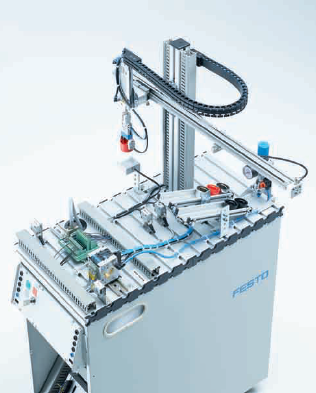
\includegraphics[scale=0.25]{HandlingStationFesto.png}
					\caption{Ο σταθμός αποθήκευσης \cite{OverviewMPSStations} {\footnotesize Παρατηρείται ότι η διάταξη μεταφοράς κινείται σε έναν άξονα μόνο και αντί για στοίβες διαθέτει πλατφόρμες κύλισης σε αντίθεση με το κείμενο. Καταγράψαμε την διάταξη ως συνδυασμό των \cite{FestoMPSHandlingStationManual} και \cite{ΤοΦυσικόΣύστημαFestoMPS} με σκοπό την χρησιμοποίηση εξαρτημάτων από ποικίλα επιστημονικά πεδία. Η εικόνα παρατίθεται μόνο για να βοηθήσει να οπτικοποιηθεί το εν λόγω σύστημα}}
					\label{φωτ:Ο σταθμός αποθήκευσης από Festo}
				\end{figure}
				
				\paragraph{Μονάδα μεταφοράς\index{μονάδα!μεταφοράς}} {Η μονάδα αυτή αποτελείται από ένα σύστημα μετακίνησης σε τρεις άξονες. Η μετακίνηση στο οριζόντιο επίπεδο επιτυγχάνεται με ηλεκτρικούς κινητήρες συνεχούς ρεύματος.Για την μετακίνηση στον κάθετο άξονα χρησιμοποιείται ένα πνευματικό έμβολο\index{έμβολο!πνευματικό} δύο κατευθύνσεων το οποίο διαθέτει μία δαγκάνα\index{δαγκάνα!πνευματική} στο άκρο του. Το έμβολο αυτό διαθέτει δύο μαγνητικούς αισθητήρες για την διαπίστωση των ακραίων θέσεων του. Η δαγκάνα κλείνει και ανοίγει με πεπιεσμένο αέρα διαθέτοντας επιπλέον και ένα οπτικό αισθητήρα ενσωματωμένο στο σώμα της για να ανιχνεύεται το κυλινδρικό τεμάχιο και το χρώμα αυτού.
				}
				
				\paragraph{Μονάδα αποθήκευσης\index{μονάδα!αποθήκευσης}} {Η μονάδα αυτή αποτελείται απλούστατα από τρεις (3) στοίβες όπως φαίνονται και στην εικόνα \ref{φωτ:Ο σταθμός αποθήκευσης από Θραμπο} χωρητικότητας οχτώ (8) τεμαχίων η καθεμία.
				}
				
				\paragraph{Ανάλυση λειτουργίας} {Λεπτομερέστερα οι προϋποθέσεις για να λειτουργήσει ο σταθμός αυτός και η σειρά με την οποία εκτελούνται οι επιμέρους ενέργειες απαριθμούνται στον πίνακα \ref{πιν.:Ανάλυση λειτουργίας του σταθμού αποθήκευσης}:
				}
				\begin{longtable} { m{0.5cm} m{12cm} }
					\caption [Ανάλυση λειτουργίας του σταθμού αποθήκευσης]  {Ανάλυση λειτουργίας του σταθμού αποθήκευσης \cite{FestoMPSHandlingStationManual}}
					\label{πιν.:Ανάλυση λειτουργίας του σταθμού αποθήκευσης}\\
					\hline
					\endfirsthead
					\multicolumn{2}{c}{συνέχεια του πίνακα \ref{πιν.:Ανάλυση λειτουργίας του σταθμού αποθήκευσης}}\\
					\hline
					~\\
					\endhead
					\hline
					\multicolumn{2}{c}{ο πίνακας συνεχίζεται στην επόμενη σελίδα}\\
					\endfoot
					\multicolumn{2}{c}{ολοκληρώθηκε ο πίνακας \ref{πιν.:Ανάλυση λειτουργίας του σταθμού αποθήκευσης}}\\
					\endlastfoot
					~\\
					\multicolumn{2}{c}{Προαπαιτήσεις}\\
					1 & Κυλινδρικό τεμάχιο υπάρχει στην θέση παράδοσης του περιστρεφόμενου δίσκου\\
					\hline
					~\\
					\multicolumn{2}{c}{Αρχική κατάσταση}\\
					1 & Το έμβολο του πνευματικού κυλίνδρου βρίσκεται σε θέση σύμπτυξης\\
					2 & Η διάταξη βεντούζας-εμβόλου βρίσκεται στη θέση ηρεμίας.\\
					\hline
					~\\
					\multicolumn{2}{c}{Ακολουθία ενεργειών}\\
					1 & Εντοπίζεται τεμάχιο έτοιμο προς αποθήκευση.\\
					2 & Η διάταξη μεταφοράς μεταβαίνει στη θέση παράδοσης του δίσκου, εφόσον έχει πατηθεί και το πλήκτρο της εκκίνησης.\\
					3 & Το έμβολο αναπτύσσεται.\\
					4 & Η δαγκάνα κλείνει.\\
					5 & Το έμβολο συμπτύσσεται.\\
					   & Περίπτωση μαύρου τεμαχίου.\\
					6 & Η διάταξη μεταφοράς μεταβαίνει στη στοίβα 1 (εσωτερική).\\
					7 & Το έμβολο αναπτύσσεται.\\
					8 & Η δαγκάνα ανοίγει και το τεμάχιο πέφτει μέσα στη στοίβα.\\
					9 & Το έμβολο συμπτύσεται.\\
					10 & Η διάταξη μεταφοράς μεταβαίνει στη θέση ηρεμίας.\\
					    & Περίπτωση κόκκινο ή ασημένιου στο χρώμα τεμαχίου.\\
					11 & Η διάταξη μεταφοράς μεταβαίνει στη στοίβα 2 (μεσαία).\\
					12 & Το έμβολο αναπτύσσεται.\\
					13 & Η δαγκάνα ανοίγει και το τεμάχιο πέφτει μέσα στη στοίβα.\\
					14 & Το έμβολο συμπτύσεται.\\
					15 & Η διάταξη μεταφοράς μεταβαίνει στη θέση ηρεμίας.\\
					    & Περίπτωση μη αποδεκτής διάτρησης.\\
					16 & Η διάταξη μεταφοράς μεταβαίνει στη στοίβα 3 (εξωτερική).\\
					17 & Το έμβολο αναπτύσσεται.\\
					18 & Η δαγκάνα ανοίγει και το τεμάχιο πέφτει μέσα στη στοίβα.\\
					19 & Το έμβολο συμπτύσεται.\\
					20 & Η διάταξη μεταφοράς μεταβαίνει στη θέση ηρεμίας.\\
					\hline
				\end{longtable}

%%%%%%%%%%%%%%%%%%%%%%%%%%%%%%%%%%%%%%%%%%%%%%%%%%%%%%%%%%%%%
%%%%%%%%%%%%%%		   								 Ενότητα		   					   %%%%%%%%%%%%%%%%%%%%
%%%%%%%%%%%%%%%%%%%%%%%%%%%%%%%%%%%%%%%%%%%%%%%%%%%%%%%%%%%%%
		\section{Μοντελοποίηση του συστήματος}
		
			\paragraph{} {Για τη μοντελοποίηση του συστήματος χρησιμοποιήσαμε μία παραλλαγή του V μοντέλου. Στο πρώτο στάδιο καταγράψαμε τις απαιτήσεις της ομάδας παραγγελίας. Στο δεύτερο κατασκευάσαμε ένα γενικό λογικό μοντέλο του συστήματος. Το μοντέλο αυτό κατασκευάστηκε με τέτοιο τρόπο ώστε να ειναι ανεξάρτητο των τεχνολογίών υλοποίησης, Το τρίτο στάδιο περιλαμβάνει το μοντέλο υλοποίησης στο οποίο περιγράφεται λεπτομερώς το σύστημα. Σε αυτό καταγράφονται οι τεχνολογίες υλοποίησης ώστε να απεικονίζεται η αλληλεπίδραση των διαφόρων επιστημονικών πεδιων.
			}

%%%%%%%%%%%%%%%%%%%%%%%%%%%%%%%%%%%%%%%%%%%%%%%%%%%%%%%%%%%%%
%%%%%%%%%%%%%%		   							Υποενότητα		   					   %%%%%%%%%%%%%%%%%%%%
			\subsection{Μοντέλο Σύλληψης\index{μοντέλο!σύλληψης} - Conception Model\index{model!conception}}
			
				\paragraph{} {Το μοντέλο αυτό χρησιμοποιήθηκε για την πρωταρχική περιγραφή του συστήματος και την καταγραφή των απαιτήσεων της ομάδας παραγγελίας.
				}
			
%%%%%%%%%%%%%%%%%%%%%%%%%%%%%%%%%%%%%%%%%%%%%%%%%%%%%%%%%%%%%
%%%%%%%%%%%%%%		   							Υποενότητα		   					   %%%%%%%%%%%%%%%%%%%%		
			\subsection{Μοντέλο Ανάλυσης\index{μοντέλο!ανάλυσης} - Analysis Model\index{model!analysis}}
			
				\paragraph{} {Το μοντέλο αυτό χρησιμοποιήθηκε για την περαιτέρω ανάλυση του συστήματος. Στο μοντέλο αυτό δεν καταγράφονται αποφάσεις για την τελική υλοποίησή του. Συνεπώς, υπόκειται εύκολα σε τροποποιήσεις και αλλαγές στη χρησιμοποιούμενη τεχνλογία στο μοντέλο υλοποίησης.
				}			
			
%%%%%%%%%%%%%%%%%%%%%%%%%%%%%%%%%%%%%%%%%%%%%%%%%%%%%%%%%%%%%
%%%%%%%%%%%%%%		   							Υποενότητα		   					   %%%%%%%%%%%%%%%%%%%%		
			\subsection{Μοντέλο Υλοποίησης\index{μοντέλο!υλοποίησης} - Implementation Model\index{model!implementation}}
			
				\paragraph{} {Το μοντέλο αυτό παρουσιάζει το σύστημα όπως πρέπει να κατασκευαστεί. Περιλαμβάνει λεπτομέρειες για τα τελικώς χρησιμοποιούμενα εξαρτήματα καθώς και για τις τεχνολογίες που υλοποιούνται στις βιομηχανικές διεργασίες και διεργασίες ελέγχου του συστήματος. Καταγράφει όλες τις απαραίτητες κατευθύνσεις που πρέπει να δοθούν στους μηχανικούς -ηλεκτρολόγους, μηχανολόγους, μηχανικούς λογισμικού- για να κατασκευαστούν τα ανάλογα υποσυστήματα.
				}
				
				\paragraph{Σημείωση} {Στο μοτνέλο αυτό θα παρατηρήσετε ότι σε κάθε σταθμό υπάρχει ένα υποσύστημα ελέγχου το οποίο συλλέγει τις πληροφορίες από τους αισθητήρες και ελέγχει τους ενεργοποιητές και τις μονάδες λειτουργιας. Το σύστημα αυτό έχει μοντελοποιηθεί ως σύστημα που εκτελεί Java κώδικα. Αυτό δεν ισχύει στο πραγματικό σύστημα. Αντιθέτως, στην πραγματικότητα χρησιμοποιείται μία μονάδα PLC. Στο κατασκευασθέν μοντέλο χρησιμοποιήθηκε η Java μονάδα λόγω συμβατότητας με τον εξομοιωτή FestoMPS. Επεξηγώντας, το πραγματικό σύστημα δεν είναι διαθέσιμο σε εμάς. Συνεπώς, κατασκευάστηκε σε λογισμικό ένας εξομοιωτής του συστήματος που χρησιμοποιεί java τεχνολογίες {\footnotesize (βλπ. \ref{Έλεγχος του συστήματος ελέγχου του Festo MPS}}
				}
				
%%%%%%%%%%%%%%%%%%%%%%%%%%%%%%%%%%%%%%%%%%%%%%%%%%%%%%%%%%%%%
%%%%%%%%%%%%%%		   							Υποενότητα		   					   %%%%%%%%%%%%%%%%%%%%
			\subsection{Μοντέλο Συστήματος Ελέγχου\index{μοντέλο!συστήματος ελέγχου}}
			
				\paragraph{} {Χάρη στο μοντέλο υλοποίησης το οποίο διαθέτουμε ως είσοδο στο μοντέλο του συστήματος ελέγχου του Festo MPS\textregistered, διακρίνουμε τα παρακάτω στοιχεία αλληλεπίδρασης του συστήματος ελέγχου και των υπολοίπων μονάδων.
				}
				
				\begin{longtable} { m{2.5cm} m{10cm} }
					\caption [Αισθητήρες και ενεργοποιητές του Festo MPS]  {Αισθητήρες και ενεργοποιητές του Festo MPS}
					\label{πιν.:Αισθητήρες και ενεργοποιητές του Festo MPS}\\
					\endfirsthead
					\multicolumn{2}{c}{συνέχεια του πίνακα \ref{πιν.:Αισθητήρες και ενεργοποιητές του Festo MPS}}\\
					~\\
					\endhead
					\hline
					\multicolumn{2}{c}{ο πίνακας συνεχίζεται στην επόμενη σελίδα}\\
					\endfoot
					\hline
					\multicolumn{2}{c}{ολοκληρώθηκε ο πίνακας \ref{πιν.:Αισθητήρες και ενεργοποιητές του Festo MPS}}\\
					\endlastfoot
					~\\
					\multicolumn{2}{c}{Σταθμός διανομής}\\
					\hline
					~\\
					\multicolumn{2}{l}{Στοίβα με πνευματικό έμβολο}\\
					\multirow{3}*{Αισθητήρες} & Αισθητήρας πίσω θέσης του εμβόλου\\
														 & Αισθητήρας μπροστινής θέσης του εμβόλου\\
														 & Αισθητήρας κυλινδρικού τεμαχίου\\
					Ενεργοποιητές & Βαλβίδα 5/2\\
					\hline
					~\\
					\multicolumn{2}{l}{Μονάδα μεταφοράς}\\
					\multirow{3}*{Αισθητήρες} & Αισθητήρας κενού\\
														 & Αισθητήρας αριστερής τοποθέτησης του βραχίονα\\
														 & Αισθητήρας δεξιάς τοποθέτησης του βραχίονα\\
					\multirow{3}*{Ενεργοποιητές} & Βαλβίδα μη επιστροφής\\
															  & Ενεργοποίηση της βαλβίδας 5/3 για αριστερή τοποθέτηση του βραχίονα\\
															  & Ενεργοποίηση της βαλβίδας 5/3 για δεξιά τοποθέτηση του βραχίονα\\
					\hline
					~\\
					\multicolumn{2}{c}{Σταθμός ελέγχου}\\
					\hline
					~\\
					\multicolumn{2}{l}{Ανελκυστήρας}\\
					\multirow{7}*{Αισθητήρες} & Αισθητήρας άνω θέσης του ανελκυστήρα\\
														 & Αισθητήρας χαμηλής θέσης του ανελκυστήρα\\
														 & Αισθητήρας διάχυσης\\
														 & Αισθητήρας χωρητικός\\
														 & Αισθητήρας ανακλαστικός\\
														 & Αισθητήρας μπροστινής θέσης του εμβόλου\\
														 & Αισθητήρας πίσω θέσης του εμβόλου\\
					\multirow{2}*{Ενεργοποιητές} & Βαλβίδα 5/2 ανελκυστήρα\\
															  & Βαλβίδα 5/2 εμβόλου\\
					\hline
					~\\
					\multicolumn{2}{c}{Σταθμός επεξεργασίας}\\
					\hline
					~\\
					\multicolumn{2}{l}{Περιστρεφόμενος δίσκος}\\
					\multirow{4}*{Αισθητήρες} & Αισθητήρας επαγωγικός\\
														 & Αισθητήρας χωρητκός θέσης υποδοχής\\
														 & Αισθητήρας χωρητκός θέσης διάτρησης\\
														 & Αισθητήρας χωρητκός θέσης μέτρησης\\
					Ενεργοποιητές & Ηλεκτρικό ρελέ\\
					\hline
					~\\
					\multicolumn{2}{l}{Μονάδα διάτρησης}\\
					\multirow{4}*{Αισθητήρες} & Αισθητήρας μπροστινής θέσης του εμβόλου\\
														 & Αισθητήρας πίσω θέσης του εμβόλου\\
														 & Αισθητήρας άνω θέσης του τρυπανιού\\
														 & Αισθητήρας χαμηλής θέσης του τρυπανιού\\
					\multirow{4}*{Ενεργοποιητές} & Ηλεκτρικό ρελέ τρυπανιού\\
															  & Ηλεκτρικό ρελέ ανερχόμενης κίνησης τρυπανιού\\
															  & Ηλεκτρικό ρελέ κατερχόμενης κίνησης τρυπανιού\\
															  & Βαλβίδα 5/2 εμβόλου\\
					\hline
					~\\
					\multicolumn{2}{l}{Μονάδα μέτρησης}\\
					\multirow{2}*{Αισθητήρες} & Αισθητήρας άνω θέσης της ακίδας\\
													 	 & Αισθητήρας χωρητικός ως ακίδα\\
					Ενεργοποιητές & Ηλεκτρικό ρελέ κατερχώμενης κίνησης της ακίδας\\
					\hline
					~\\
					\multicolumn{2}{c}{Σταθμός αποθήκευσης}\\
					\hline
					~\\
					\multicolumn{2}{l}{Μονάδα μεταφοράς}\\
					\multirow{3}*{Αισθητήρες} & Αισθητήρας διάχυσης\\
														 & Αισθητήρας χαμηλής θέσης του εμβόλου\\
														 & Αισθητήρας άνω θέσης του εμβόλου\\
					\multirow{6}*{Ενεργοποιητές} & Ηλεκτρικό ρελέ ορθής κίνησης κινητήρα Χ διεύθυνσης\\
															  & Ηλεκτρικό ρελέ ανάστροφης κίνησης κινητήρα Χ διεύθυνσης\\
															  & Ηλεκτρικό ρελέ ορθής κίνησης κινητήρα Υ διεύθυνσης\\
															  & Ηλεκτρικό ρελέ ανάστροφής κίνησης κινητήρα Υ διεύθυνσης\\
															  & Βαλβίδα 5/2 εμβόλου\\
															  & Βαλβίδα 5/2 δαγκάνας\\
					\hline
				\end{longtable}
				
%%%%%%%%%%%%%%%%%%%%%%%%%%%%%%%%%%%%%%%%%%%%%%%%%%%%%%%%%%%%%
%%%%%%%%%%%%%%		   								 Ενότητα		   					   %%%%%%%%%%%%%%%%%%%%
%%%%%%%%%%%%%%%%%%%%%%%%%%%%%%%%%%%%%%%%%%%%%%%%%%%%%%%%%%%%%	
		\section{Έλεγχος του συστήματος ελέγχου του Festo MPS}
			\label{Έλεγχος του συστήματος ελέγχου του Festo MPS}
		
			\paragraph{} {Για τον εξακρίβωση της ορθής λειτουργίας του συστήματος ελέγχου αναπτύχθηκε ένας εξομοιωτής του Festo MPS\textregistered λόγω της αδιαθεσιμότητας του πραγματικού συστήματος. Ο εξομοιωτής έχει υλοποιηθεί χρησιμοποιώντας τη γλώσσα προγραμματισμού Java στο περιβάλλον Netbeans\footnote{http://www.http://netbeans.org/}. Για την επικοινωνία του συστήματος ελέγχου με τον εξομοιωτή έγινε χρήση της τεχνολογίας των sockets, που υποστηρίζει η Java ως μέθοδος επικοινωνίας μέταξύ εφαρμογών που τρέχουν πάνω σε διαφορετικά συστήματα του ίδιου δικτύου.
			}
			

%%%%%%%%%%%%%%%%%%%%%%%%%%%%%%%%%%%%%%%%%%%%%%%%%%%%%%%%%%%%%
%%%%%%%%%%%%%%		   								 Κεφάλαιο		   					   %%%%%%%%%%%%%%%%%%%%
%%%%%%%%%%%%%%%%%%%%%%%%%%%%%%%%%%%%%%%%%%%%%%%%%%%%%%%%%%%%%
%%%%%%%%%%%%%%%%%%%%%%%%%%%%%%%%%%%%%%%%%%%%%%%%%%%%%%%%%%%%%
	\chapter{Δεύτερο πεδίο εφαρμογής :\\ Takos System}
		\label{κεφ.:Δεύτερο πεδίο εφαρμογής : Takos System}

%%%%%%%%%%%%%%%%%%%%%%%%%%%%%%%%%%%%%%%%%%%%%%%%%%%%%%%%%%%%%
%%%%%%%%%%%%%%		   								 Κεφάλαιο		   					   %%%%%%%%%%%%%%%%%%%%
%%%%%%%%%%%%%%%%%%%%%%%%%%%%%%%%%%%%%%%%%%%%%%%%%%%%%%%%%%%%%
%%%%%%%%%%%%%%%%%%%%%%%%%%%%%%%%%%%%%%%%%%%%%%%%%%%%%%%%%%%%%
	\chapter{Συμπεράσματα}
		\label{κεφ.:Συμπεράσματα}

%%%%%%%%%%%%%%%%%%%%%%%%%%%%%%%%%%%%%%%%%%%%%%%%%%%%%%%%%%%%%
%%%%%%%%%%%%%%		   								 Ενότητα		   					   %%%%%%%%%%%%%%%%%%%%
%%%%%%%%%%%%%%%%%%%%%%%%%%%%%%%%%%%%%%%%%%%%%%%%%%%%%%%%%%%%%	
		\section{Συμφωνούμε με τα παρακάτω}
			\begin{itemize}
				\item The main challenge in the case study was to understand the requirements and the functional design of the PTME system from the documents that were provided as input for the case study. Once these were understood, it was a relatively easy task to create the SysML model. \cite{SMSpacecraft}
				\item Modelling the structure of the PTME system using block definition diagrams and internal block diagrams was straight forward and consumed relative little time. \cite{SMSpacecraft}
				\item Capturing the behavioural aspects of the system was the most time-consuming part of the work. For each block diagram, several actions were modelled using activity diagrams. The activity diagrams provided an efficient means for modelling data flow and interactions between different blocks.  \cite{SMSpacecraft}
				\item  SysML follows a profile based approach to extend the language, this feature enhance the capability of system to add more domain-specific stereotypes to customize the language and reuse purposes. To expand the profile it’s very important to create meaningful stereotypes. Knowledge and experiences of system engineering are needed to define these new constructs. \cite{SMSpacecraft}
				\item Allocation of the system requirements and mapping them to each other as well blocks and activities enhances traceability. This capability of SysML is used to keep track of changes either in the requirement’s specification or the component models. The language does not provide any guidance for how to map requirements to model elements, so the modeller should preferably be an expert in the field of requirements engineering. Sometimes it is awkward to capture requirements as a block in a Requirements diagram. The alternative is to use the tables and matrixes. There, we can capture the relation just by adding more columns. \cite{SMSpacecraft}
				\item Traceability of Requirements, Specification for Sub-Systems, Verification and Validation (If the interfaces to the sub-systems and the delivered data are specied, the SysML model can be used to check whether this is enough to fulll the requirements. In TopCased, this is done via formal analysis of the system using a transformation into the formal immediate language FIACRE and using model checking techniques to verify the desired properties.), Testing and Test Case Generation, Benefits for Digital Engineering (Overall, all these reasons are very benefcial for digital engineering. The rigorous specifcation of interfaces and exchanged information as well as the specifcation of the information flow, minimizes the possibility of incompatible subsystem development. The resulting systems can easily be used for simulation and testing purpose in a virtual environment, as far as the dynamic behavior of the system is specifed. This allows for hardware in the loop tests for external sub-systems e.g., for the camera systems or software in the loop tests, delivering test data for the secure data storage system. The requirements mapping defnes in which system components the desired requirements (and sub-equirements) are implemented, therefore creating clarity about responsibilities for the correct implementation and specifcation of the interfaces and desired behavior. This makes it and wellsuited approach for interdisciplinary systems development.).\cite{SysMLDigitalEngineering}.
			\end{itemize}
			



%%%%%%%%%%%%%%%%%%%%%%%%%%%%%%%%%%%%%%%%%%%%%%%%%%%%%%%%%%%%%
%%%%%%%%%%%%%%		   								 Ενότητα		   					   %%%%%%%%%%%%%%%%%%%%
%%%%%%%%%%%%%%%%%%%%%%%%%%%%%%%%%%%%%%%%%%%%%%%%%%%%%%%%%%%%%	
		\section{Σχεδίαση βάση εξομείωσης}
			\paragraph{Η σχεδίαση βάση εξομείωσης} {ή κατά την αγγλική ορολογία simulation-based design μπορεί να βασιστεί στα διαγράμματα παραμέτρων που παράγονται με τη SysML και να εξομειωθούν με τα κατάλληλα εργαλία. \cite{SimBasedDesignP1} και \cite{SimBasedDesignP2}
			}

%%%%%%%%%%%%%%%%%%%%%%%%%%%%%%%%%%%%%%%%%%%%%%%%%%%%%%%%%%%%%
%%%%%%%%%%%%%%		   								 Ενότητα		   					   %%%%%%%%%%%%%%%%%%%%
%%%%%%%%%%%%%%%%%%%%%%%%%%%%%%%%%%%%%%%%%%%%%%%%%%%%%%%%%%%%%			
		\section{SoC, SysML and SystemC}
			\paragraph{Copying from \cite{SoCSysMLSystemC} : } {In this paper we have presented a SysML profile for modeling Systems on a Chip oriented to SystemC transformation. We have shown that by means of SysML diagrams like BDD, IBD, and Activity allocations it is possible to describe a SoC and then map the SoC descriptions to a SystemC code template which contains module definitions, port- and process declarations. We also described a possible SysML to SystemC transformation procedure based on XMI and XSLT rules that we would like to automate within our future work. The SysML-SystemC mapping has been also evaluated by means of a case study in the field of WSN and a possible SystemC code has been derived from SysML diagrams describing a Sensor Node. This work would like to give a first contribution towards a research topic that has not been investigated so far, namely SysML to SystemC transformation. In fact there is a lot of research works available in the field of UML to SystemC, but nothing within SysML to SystemC. Since we strongly believe that SysML is a very suitable modeling language for SoC design, we think that the transformation from SysML to SystemC is a very important step within an early system design phase.
			}

%%%%%%%%%%%%%%%%%%%%%%%%%%%%%%%%%%%%%%%%%%%%%%%%%%%%%%%%%%%%%
%%%%%%%%%%%%%%		   								 Ενότητα		   					   %%%%%%%%%%%%%%%%%%%%
%%%%%%%%%%%%%%%%%%%%%%%%%%%%%%%%%%%%%%%%%%%%%%%%%%%%%%%%%%%%%			
		\section{The processing system paradigm}
			\paragraph{Copying from \cite{ProcessingSysPar}} {Model-based systems engineering and graphical notations have an enormous potential for increasing design productivity, system quality and lifetime by shifting the bulk of design efforts to early phases. In spite of that this is hardly questioned, the shift towards model-based approaches has not come to a break through, as we are experiencing in software engineering. It is believed that a major reason is lack of a common system view that can act as a framework for developing modelling languages and methods for a broad community of system engineers. This paper suggests such a framework. It identifies the systems of concern as a processing system that consist of a process control system and a resource system, and applies two related views on processing systems: A functional view and a solution view. The framework has been successfully tested on telecommunication systems and networks for some years. It is believed that it holds for many other system domains as well.
			}
			
		\section{Ανάπτυξη εργαλείων σύνδεσης διαφορετικών επιστημονικών πεδίων και Έρευνα στο μετασχηματισμό μοντέλων από το ένα εργαλείο στο άλλο.}

%%%%%%%%%%%%%%%%%%%%%%%%%%%%%%%%%%%%%%%%%%%%%%%%%%%%%%%%%%%%%
%%%%%%%%%%%%%%		   								 Κεφάλαιο		   					   %%%%%%%%%%%%%%%%%%%%
%%%%%%%%%%%%%%%%%%%%%%%%%%%%%%%%%%%%%%%%%%%%%%%%%%%%%%%%%%%%%
%%%%%%%%%%%%%%%%%%%%%%%%%%%%%%%%%%%%%%%%%%%%%%%%%%%%%%%%%%%%%
	\chapter{Προοπτικές}
		\label{κεφ.:Προοπτικές}
		
		\paragraph{} {********************************************************************
		}
		


%%%%%%%%%%%%%%%%%%%%%%%%%%%%%%%%%%%%%%%%%%%%%%%%%%%%%%%%%%%%%
%%%%%%%%%%%%%%		   								 Κεφάλαιο		   					   %%%%%%%%%%%%%%%%%%%%
%%%%%%%%%%%%%%%%%%%%%%%%%%%%%%%%%%%%%%%%%%%%%%%%%%%%%%%%%%%%%
%%%%%%%%%%%%%%%%%%%%%%%%%%%%%%%%%%%%%%%%%%%%%%%%%%%%%%%%%%%%%
\begin{appendices}
	\chapter{Festo MPS\textregistered System}
	\label{κεφ.:Παράρτημα Festo MPS System}
	
		\paragraph{} {Στο παράρτημα αυτό παρατίθενται τα διαγράμματα που κατασκευάστηκαν κατά την υλοποίηση του συστήματος Festo MPS\textregistered. Υπενθυμίζεται ότι σύμφωνα με τη μεθοδολογία που ακολουθήθηκε κατασκευάστηκαν τρία μοντέλα. Το μοντέλο Σύλληψης για την αρχική και τελείως αφαιρετική υλοποίηση του συστήματος. Το μοντέλο ανάλυσης κατά το οποίο αναπτύσσεται το σύστημα και λαμβάνονται αποφάσεις ανεξαρτήτως μεθόδου και τρόπου τελικής υλοποίησης. Και τέλος το μοντέλο Υλοποίησης στο οποίο περιγράφεται το σύστημα όπως πρέπει να κατασκευαστεί με όλες τις βασικές προδιαγραφές για τις τεχνολογίες και μεθόδους υλοποίησης.
		}
%%%%%%%%%%%%%%%%%%%%%%%%%%%%%%%%%%%%%%%%%%%%%%%%%%%%%%%%%%%%%
%%%%%%%%%%%%%%		   								 Ενότητα		   					   %%%%%%%%%%%%%%%%%%%%
%%%%%%%%%%%%%%%%%%%%%%%%%%%%%%%%%%%%%%%%%%%%%%%%%%%%%%%%%%%%%	
		\FloatBarrier
		\section{Μοντέλο Σύλληψης\index{μοντέλο!σύλληψης} - Conception Model\index{model!conception}}
			
			\subsection{Χώρος υλοποίησης συστήματος\index{χώρος υλοποίησης} - Contex\index{contex}}
			
				\clearpage
				\begin{figure}[hp]
					\centering
					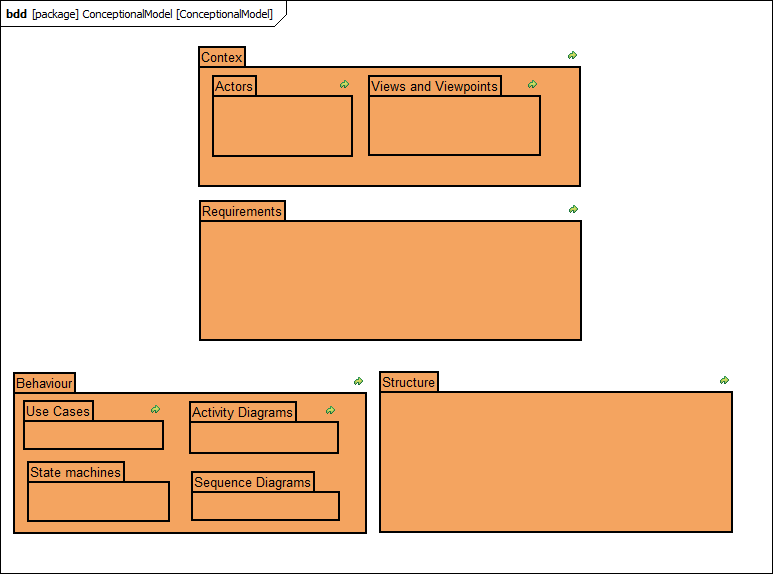
\includegraphics[scale=0.45]{ConceptionalModel_ConceptionalModel.png}
					\caption{Η δομή του μοντέλου Σύλληψης}
					\label{φωτ:Η δομή του μοντέλου Σύλληψης}
				\end{figure}
				
				\begin{figure}[hp]
					\centering
					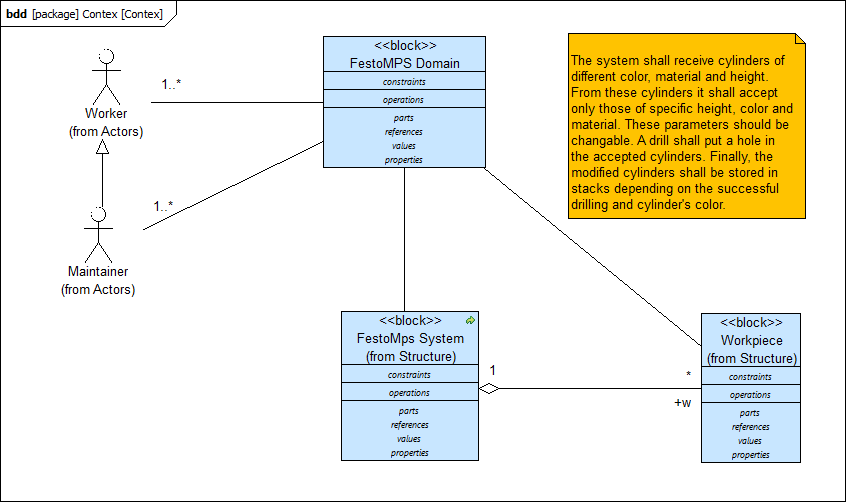
\includegraphics[scale=0.45]{ConceptionalModel_Contex.png}
					\caption{Ο χώρος υλοποίησης του μοντέλου Σύλληψης}
					\label{φωτ:Ο χώρος υλοποίησης του μοντέλου Σύλληψης}
				\end{figure}
				
				\begin{figure}[hp]
					\centering
					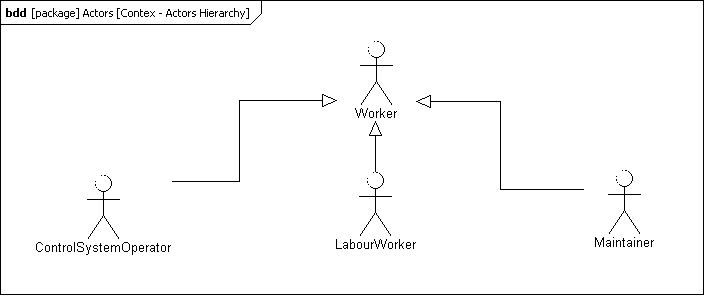
\includegraphics[scale=0.30]{ConceptionalModel_Contex-ActorsHierarchy.png}
					\caption{Οι ρόλοι του μοντέλου Σύλληψης}
					\label{φωτ:Οι ρόλοι του μοντέλου Σύλληψης}
				\end{figure}

%%%%%%%%%%%%%%%%%%%%%%%%%%%%%%%%%%%%%%%%%%%%%%%%%%%%%%%%%%%%%
%%%%%%%%%%%%%%		   							Υποενότητα		   					   %%%%%%%%%%%%%%%%%%%%
			\FloatBarrier
			\subsection{Πακέτο απαιτήσεων\index{πακέτο!απαιτήσεις}\index{απαιτήσεις!πακέτο} - Requirements package\index{requirements!package}\index{package!requirements}}
			\clearpage
				\begin{figure}[hp]
					\centering
					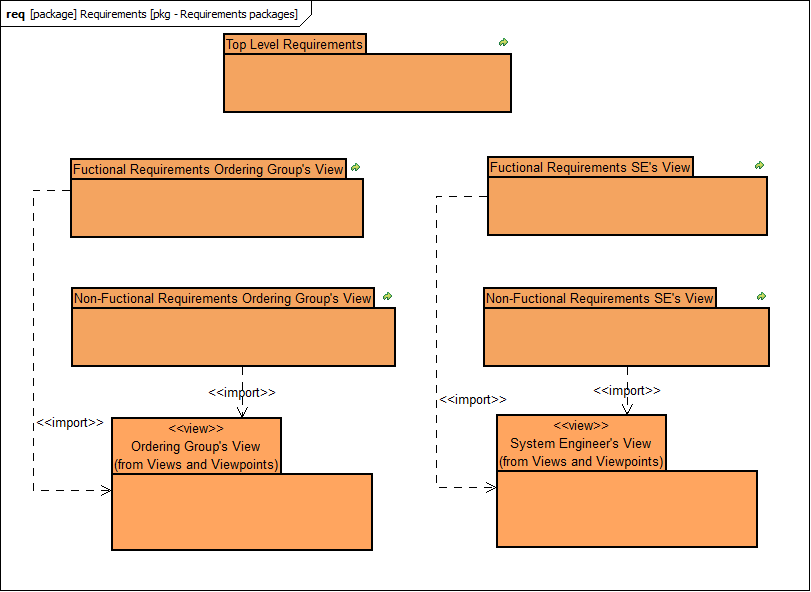
\includegraphics[scale=0.45]{ConceptionalModel_pkg-Requirementspackages.png}
					\caption{Η οργάνωση των απαιτήσεων στο μοντέλο Σύλληψης}
					\label{φωτ:Η οργάνωση των απαιτήσεων στο μοντέλο Σύλληψης}
				\end{figure}
				
				\begin{figure}[hp]
					\centering
					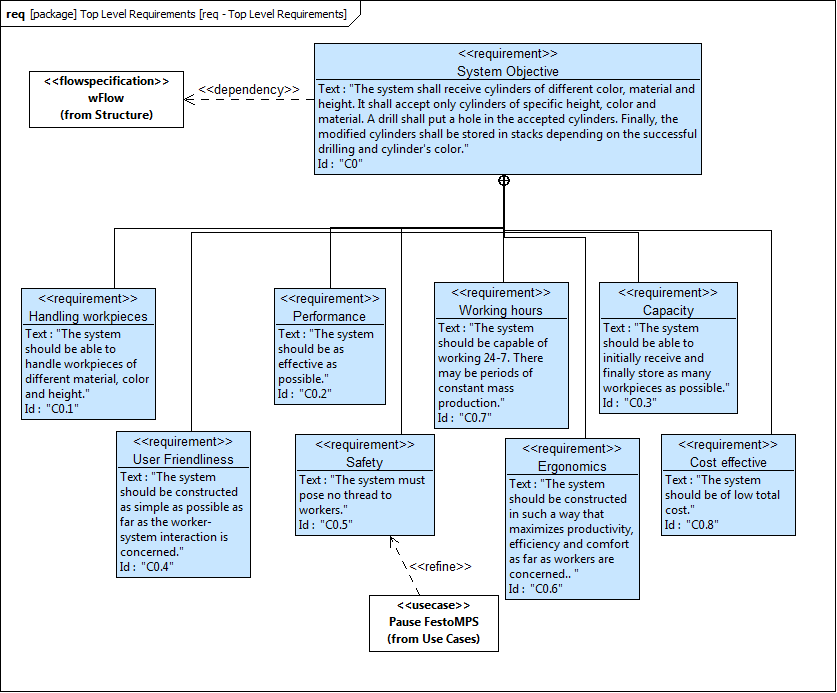
\includegraphics[scale=0.45]{ConceptionalModel_req-TopLevelRequirements.png}
					\caption{Οι γενικές απαιτήσεις του μοντέλου Σύλληψης}
					\label{φωτ:Οι γενικές απαιτήσεις του μοντέλου Σύλληψης}
				\end{figure}
				
				\begin{figure}[hp]
					\centering
					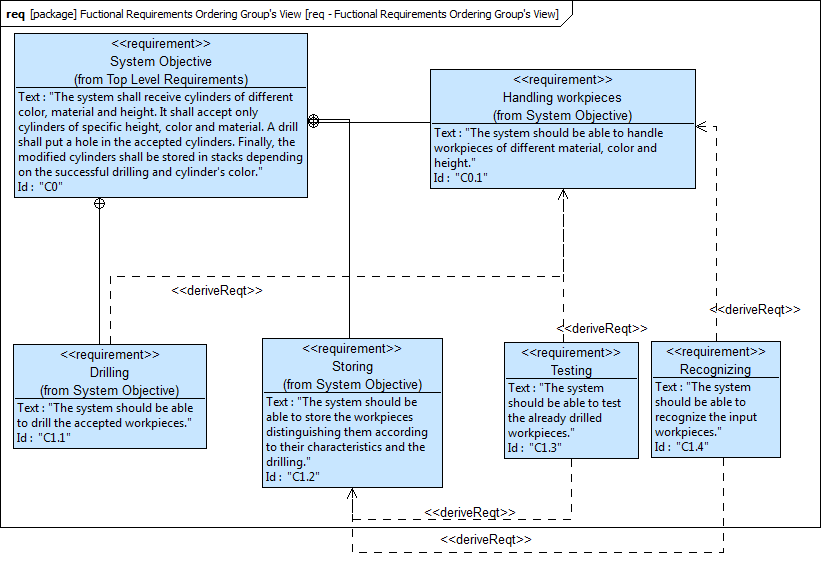
\includegraphics[scale=0.45]{ConceptionalModel_req-FuctionalRequirementsOrderingGroupsView.png}
					\caption{Οι λειτουργικές απαιτήσεις της ομάδας παραγγελίας στο μοντέλο Σύλληψης}
					\label{φωτ:Οι λειτουργικές απαιτήσεις της ομάδας παραγγελίας στο μοντέλο Σύλληψης}
				\end{figure}
				
				\begin{figure}[hp]
					\centering
					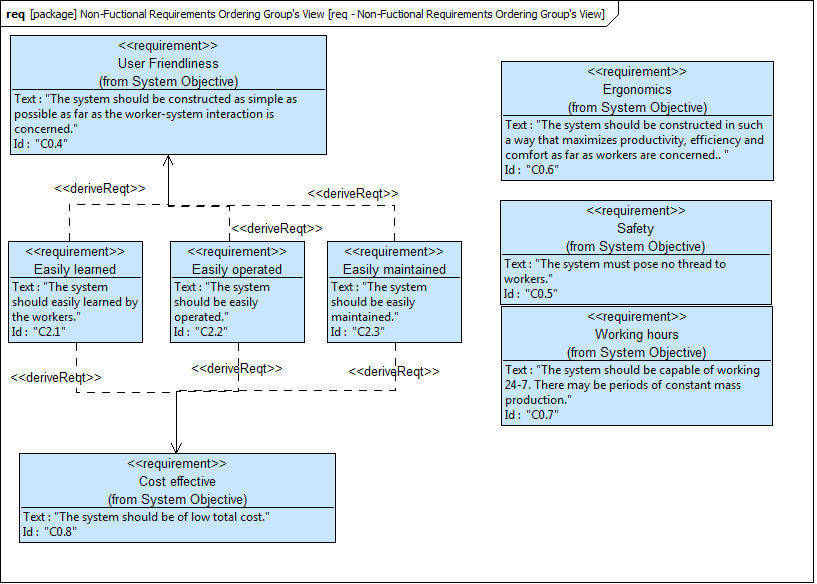
\includegraphics[scale=0.45]{ConceptionalModel_req-Non-FuctionalRequirementsOrderingGroupsView.png}
					\caption{Οι λοιπές απαιτήσεις της ομάδας παραγγελίας στο μοντέλο Σύλληψης}
					\label{φωτ:Οι λοιπές απαιτήσεις της ομάδας παραγγελίας στο μοντέλο Σύλληψης}
				\end{figure}
				
				\begin{figure}[hp]
					\centering
					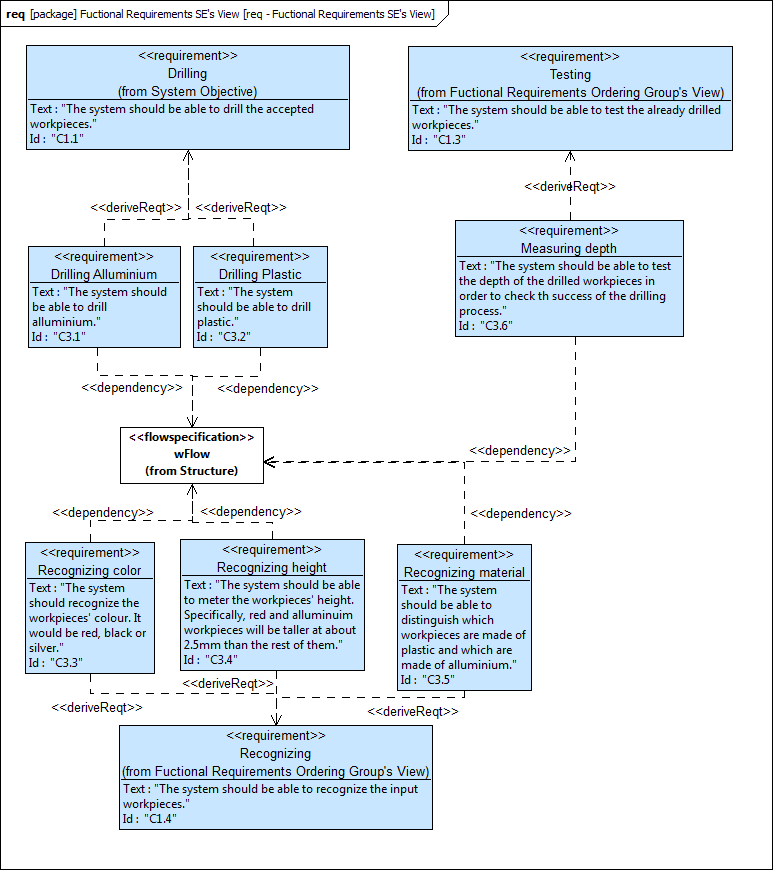
\includegraphics[scale=0.45]{ConceptionalModel_req-FuctionalRequirementsSEsView.png}
					\caption{Οι λειτουργικές απαιτήσεις του μηχανικού συστημάτων στο μοντέλο Σύλληψης}
					\label{φωτ:Οι λειτουργικές απαιτήσεις του μηχανικού συστημάτων στο μοντέλο Σύλληψης}
				\end{figure}
				
				\begin{figure}[hp]
					\centering
					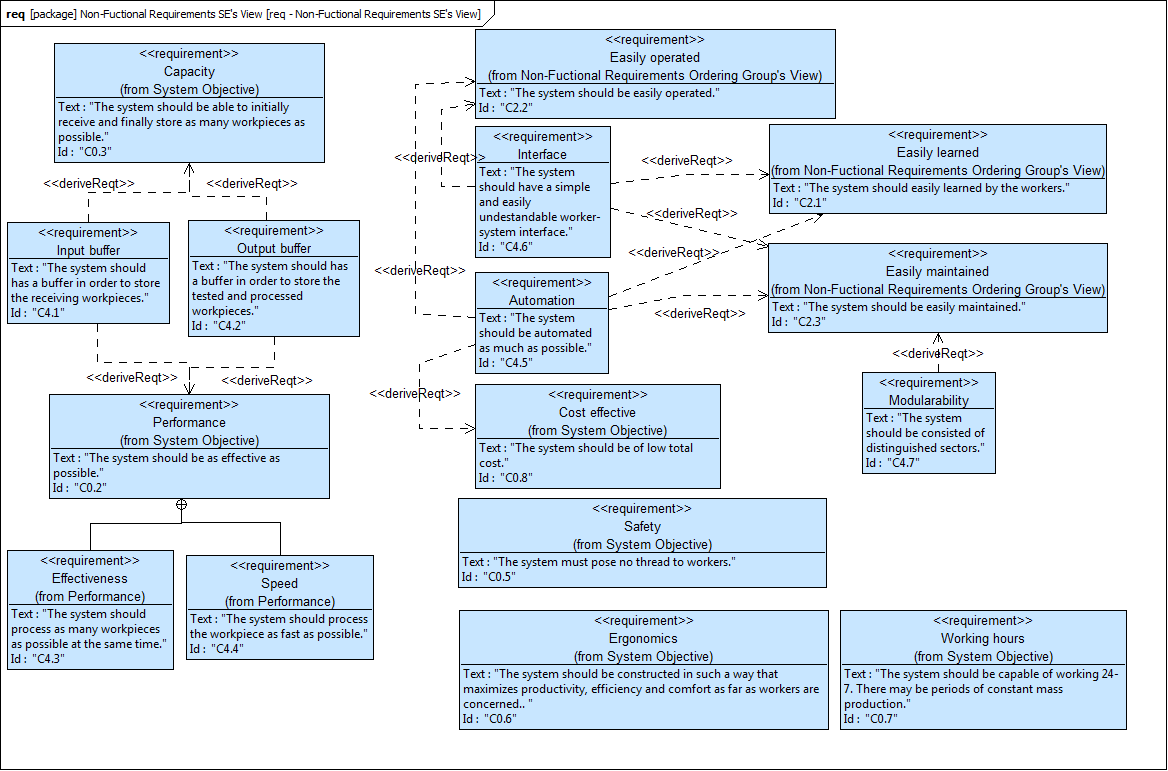
\includegraphics[scale=0.30]{ConceptionalModel_req-Non-FuctionalRequirementsSEsView.png}
					\caption{Οι λοιπές απαιτήσεις του μηχανικού συστημάτων στο μοντέλο Σύλληψης}
					\label{φωτ:Οι λοιπές απαιτήσεις του μηχανικού συστημάτων στο μοντέλο Σύλληψης}
				\end{figure}
			
%%%%%%%%%%%%%%%%%%%%%%%%%%%%%%%%%%%%%%%%%%%%%%%%%%%%%%%%%%%%%
%%%%%%%%%%%%%%		   							Υποενότητα		   					   %%%%%%%%%%%%%%%%%%%%		
			\FloatBarrier			
			\subsection{Πακέτο δομής\index{πακέτο!δομής}\index{δομή!πακέτο} - Structure package\index{structure!package}\index{package!structure}}

			\clearpage
				\begin{figure}[hp]
					\centering
					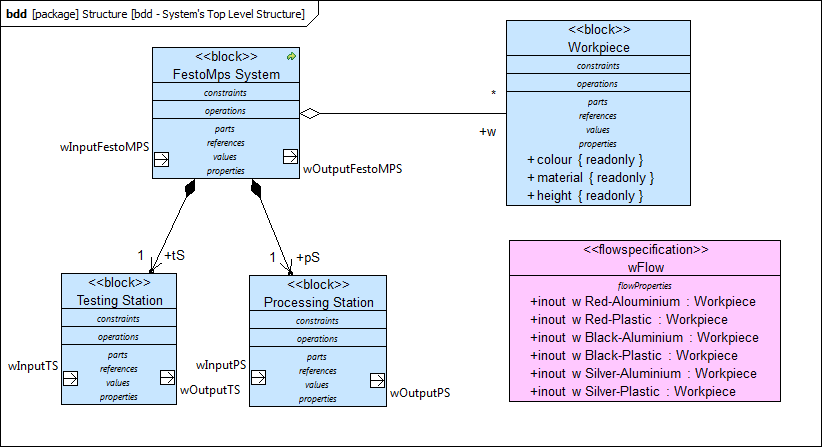
\includegraphics[scale=0.45]{ConceptionalModel_bdd-SystemsTopLevelStructure.png}
					\caption{Το bdd του συστήματος Festo MPS στο μοντέλο Σύλληψης}
					\label{φωτ:Το bdd του συστήματος Festo MPS στο μοντέλο Σύλληψης}
				\end{figure}
				\begin{figure}[hp]
					\centering
					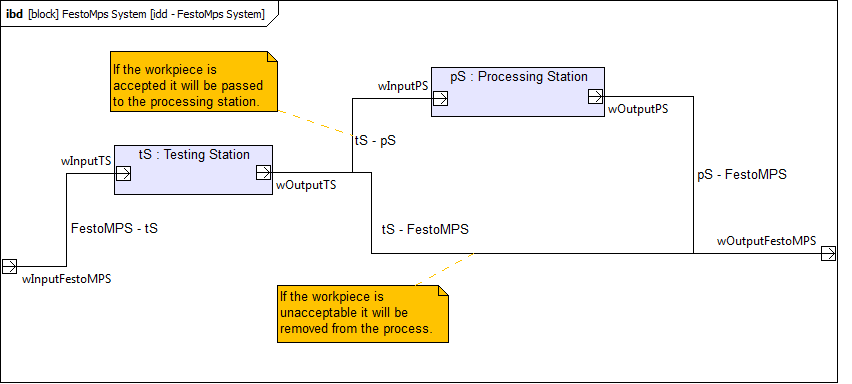
\includegraphics[scale=0.45]{ConceptionalModel_idd-FestoMpsSystem.png}
					\caption{To ibd του συστήματος Festo MPS στο μοντέλο Σύλληψης}
					\label{φωτ:To ibd του συστήματος Festo MPS στο μοντέλο Σύλληψης}
				\end{figure}
			
%%%%%%%%%%%%%%%%%%%%%%%%%%%%%%%%%%%%%%%%%%%%%%%%%%%%%%%%%%%%%
%%%%%%%%%%%%%%		   							Υποενότητα		   					   %%%%%%%%%%%%%%%%%%%%		
			\FloatBarrier
			\subsection{Πακέτο λειτουργίας\index{πακέτο!λειτουργίας}\index{λειτουργία!πακέτο} - Behaviour package\index{behavioul!package}\index{package!behaviour}}

			\clearpage
				\begin{figure}[hp]
					\centering
					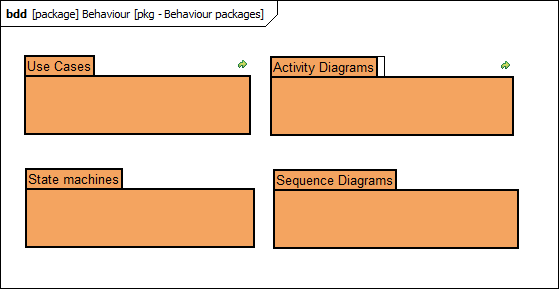
\includegraphics[scale=0.60]{ConceptionalModel_pkg-Behaviourpackages.png}
					\caption{Η οργάνωση του πακέτου λειτουργίας του συστήματος Festo MPS στο μοντέλο Σύλληψης}
					\label{φωτ: οργάνωση του πακέτου λειτουργίας του συστήματος Festo MPS στο μοντέλο Σύλληψης}
				\end{figure}
				\begin{figure}[hp]
					\centering
					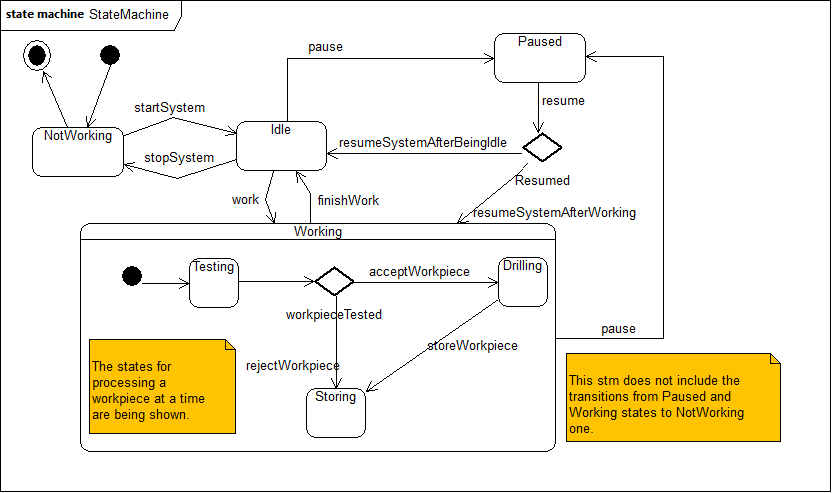
\includegraphics[scale=0.45]{ConceptionalModel_stm-SystemsTopLevelStateMachines.png}
					\caption{Οι καταστάσεις λειτουργίας του Festo MPS στο μοντέλο Σύλληψης}
					\label{φωτ:Οι καταστάσεις λειτουργίας του Festo MPS στο μοντέλο Σύλληψης}
				\end{figure}
				\begin{figure}[hp]
					\centering
					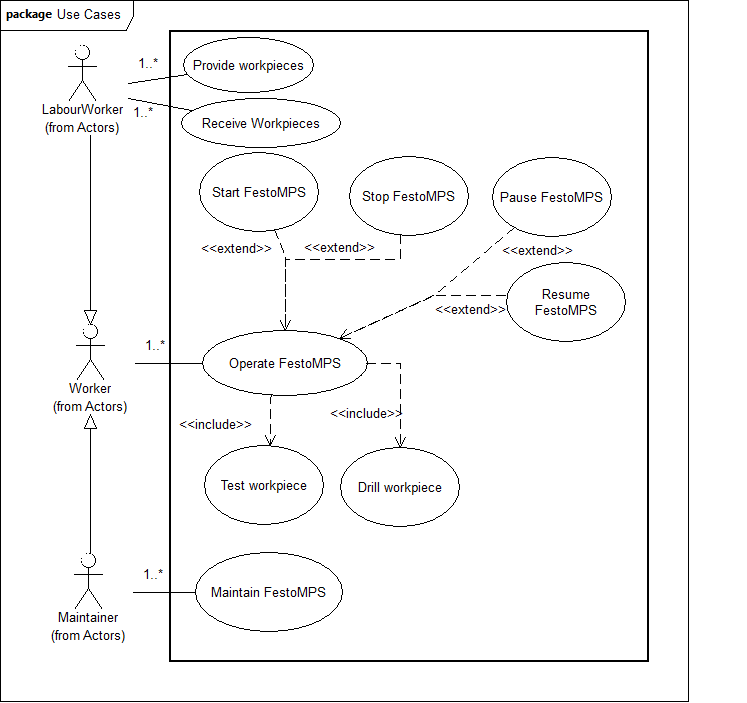
\includegraphics[scale=0.60]{ConceptionalModel_uc-SystemsTopLevelUseCases.png}
					\caption{Οι περιπτώσεις χρήσεις του Festo MPS στο μοντέλο Σύλληψης}
					\label{φωτ:Οι περιπτώσεις χρήσεις του Festo MPS στο μοντέλο Σύλληψης}
				\end{figure}
				\begin{figure}[hp]
					\centering
					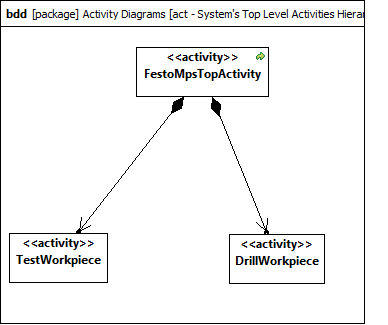
\includegraphics[scale=0.45]{ConceptionalModel_act-SystemsTopLevelActivitiesHierarchy.png}
					\caption{Η οργάνωση των Ενεργειών του Festo MPS στο μοντέλο Σύλληψης}
					\label{φωτ:Η οργάνωση των Ενεργειών του Festo MPS στο μοντέλο Σύλληψης}
				\end{figure}
				\begin{figure}[hp]
					\centering
					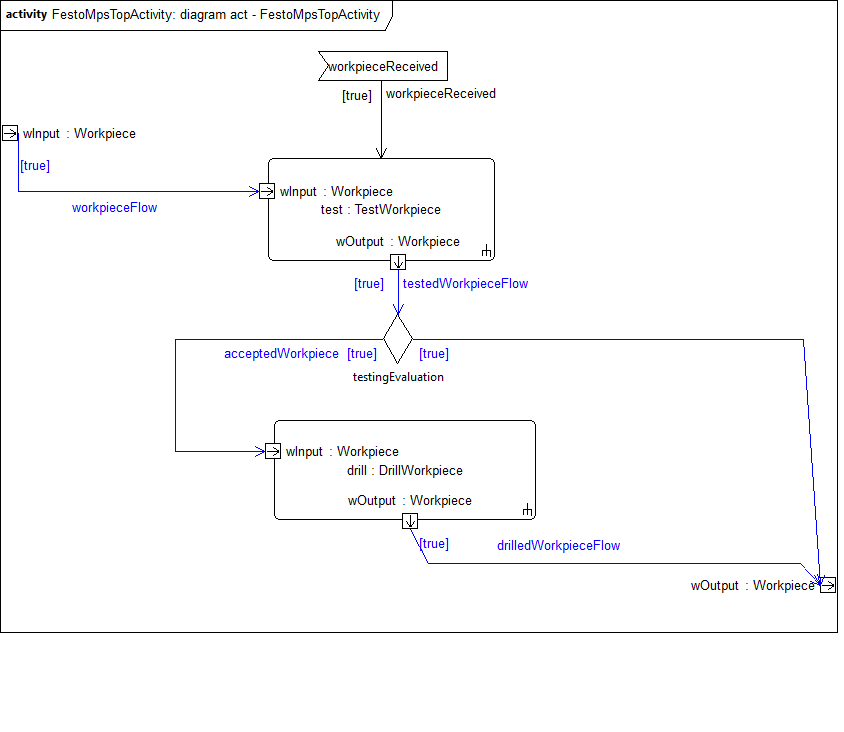
\includegraphics[scale=0.45]{ConceptionalModel_act-SystemsTopLevelActivity.png}
					\caption{Οι ενέργειες του Festo MPS στο μοντέλο Σύλληψης}
					\label{φωτ:Οι ενέργειες του Festo MPS στο μοντέλο Σύλληψης}
				\end{figure}
				\begin{figure}[hp]
					\centering
					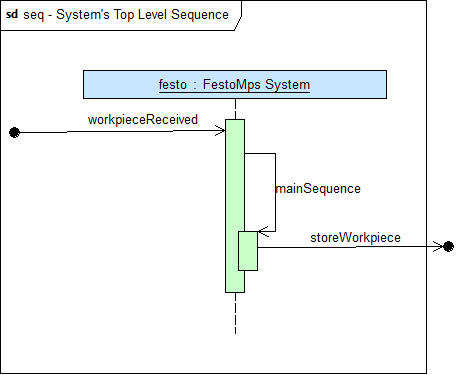
\includegraphics[scale=0.45]{ConceptionalModel_seq-SystemsTopLevelSequence.png}
					\caption{Το αφαιρετικό διάγραμμα ακολουθίας του μοντέλου Σύλληψης}
					\label{φωτ:Το αφαιρετικό διάγραμμα ακολουθίας του μοντέλου Σύλληψης}
				\end{figure}
				\begin{figure}[hp]
					\centering
					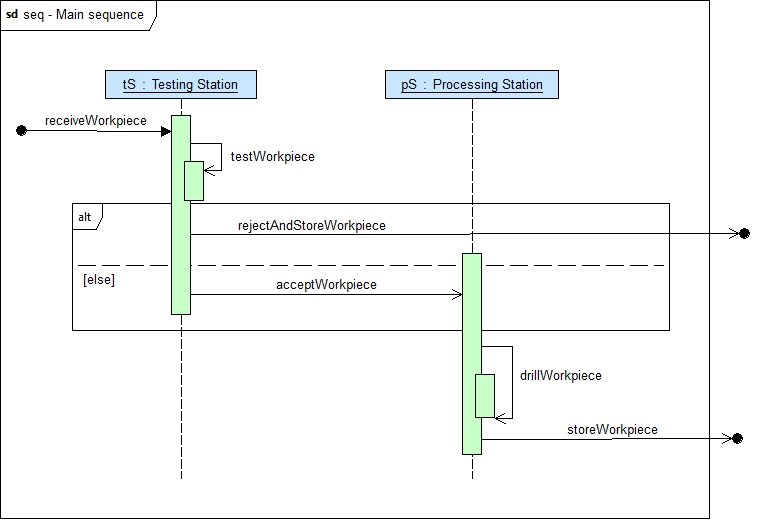
\includegraphics[scale=0.45]{ConceptionalModel_seq-MainSequence.png}
					\caption{Το διάγραμμα της κύριας ακολουθίας του Festo MPS στο μοντέλο Σύλληψης}
					\label{φωτ:Το διάγραμμα της κύριας ακολουθίας του Festo MPS στο μοντέλο Σύλληψης}
				\end{figure}

%%%%%%%%%%%%%%%%%%%%%%%%%%%%%%%%%%%%%%%%%%%%%%%%%%%%%%%%%%%%%
%%%%%%%%%%%%%%		   								 Ενότητα		   					   %%%%%%%%%%%%%%%%%%%%
%%%%%%%%%%%%%%%%%%%%%%%%%%%%%%%%%%%%%%%%%%%%%%%%%%%%%%%%%%%%%	
		\FloatBarrier		
		\section{Μοντέλο Ανάλυσης\index{μοντέλο!ανάλυσης} - Analysis Model\index{model!analysis}}
		
%%%%%%%%%%%%%%%%%%%%%%%%%%%%%%%%%%%%%%%%%%%%%%%%%%%%%%%%%%%%%
%%%%%%%%%%%%%%		   							Υποενότητα		   					   %%%%%%%%%%%%%%%%%%%%		
			\FloatBarrier
			\subsection{Χώρος υλοποίησης συστήματος\index{χώρος υλοποίησης} - Contex\index{contex}}

			\clearpage
				\begin{figure}[hp]
					\centering
					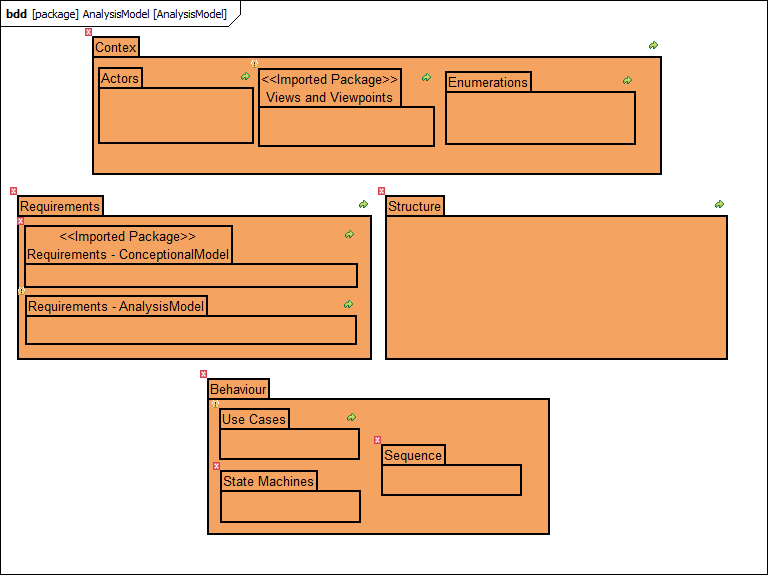
\includegraphics[scale=0.45]{AnalysisModel_AnalysisModel.png}
					\caption{Η δομή του μοντέλου Ανάλυσης}
					\label{φωτ:Η δομή του μοντέλου Ανάλυσης}
				\end{figure}
				
				\begin{figure}[hp]
					\centering
					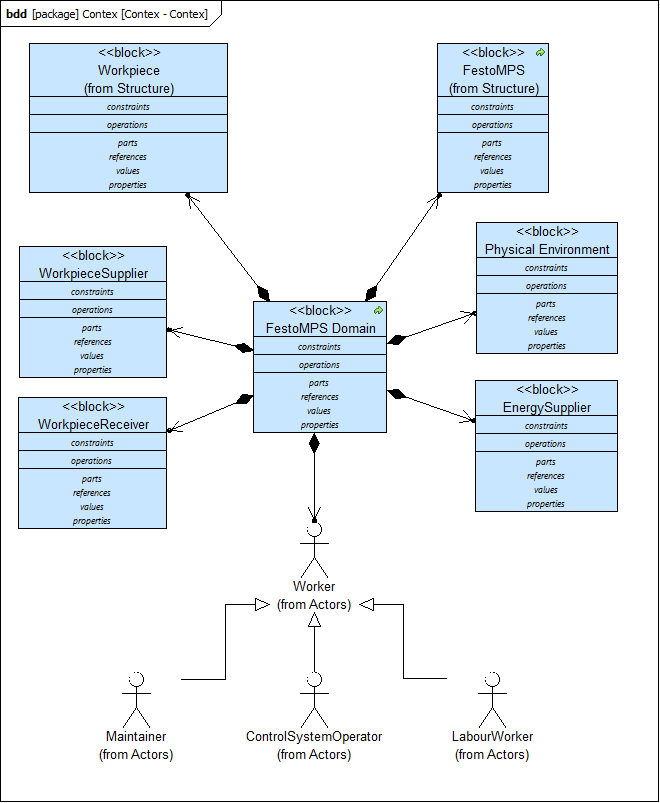
\includegraphics[scale=0.45]{AnalysisModel_Contex-Contex.png}
					\caption{Ο χώρος υλοποίησης του μοντέλου Ανάλυσης}
					\label{φωτ:Ο χώρος υλοποίησης του μοντέλου Ανάλυσης}
				\end{figure}
				
				\begin{figure}[hp]
					\centering
					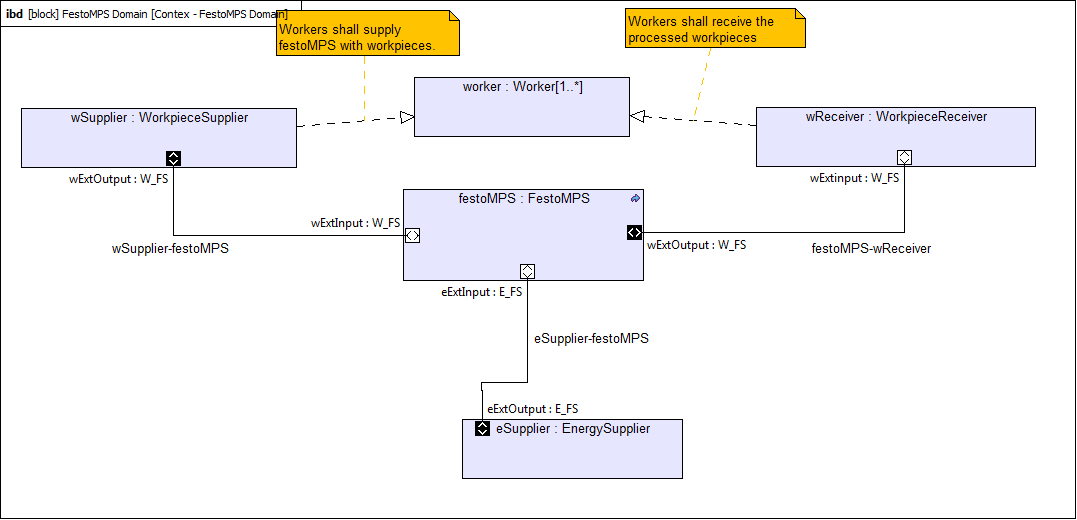
\includegraphics[scale=0.30]{AnalysisModel_Contex-FestoMPSDomain.png}
					\caption{Η σχέση του συστήματος με τον χώρο υλοποίησης του στο μοντέλο Ανάλυσης}
					\label{φωτ:Η σχέση του συστήματος με τον χώρο υλοποίησης του στο μοντέλο Ανάλυσης}
				\end{figure}
				
				\begin{figure}[hp]
					\centering
					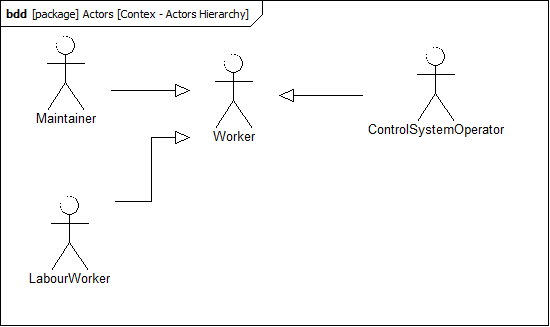
\includegraphics[scale=0.50]{AnalysisModel_Contex-ActorsHierarchy.png}
					\caption{Οι ρόλοι του μοντέλου Ανάλυσης}
					\label{φωτ:Οι ρόλοι του μοντέλου Ανάλυσης}
				\end{figure}
				
				\begin{figure}[hp]
					\centering
					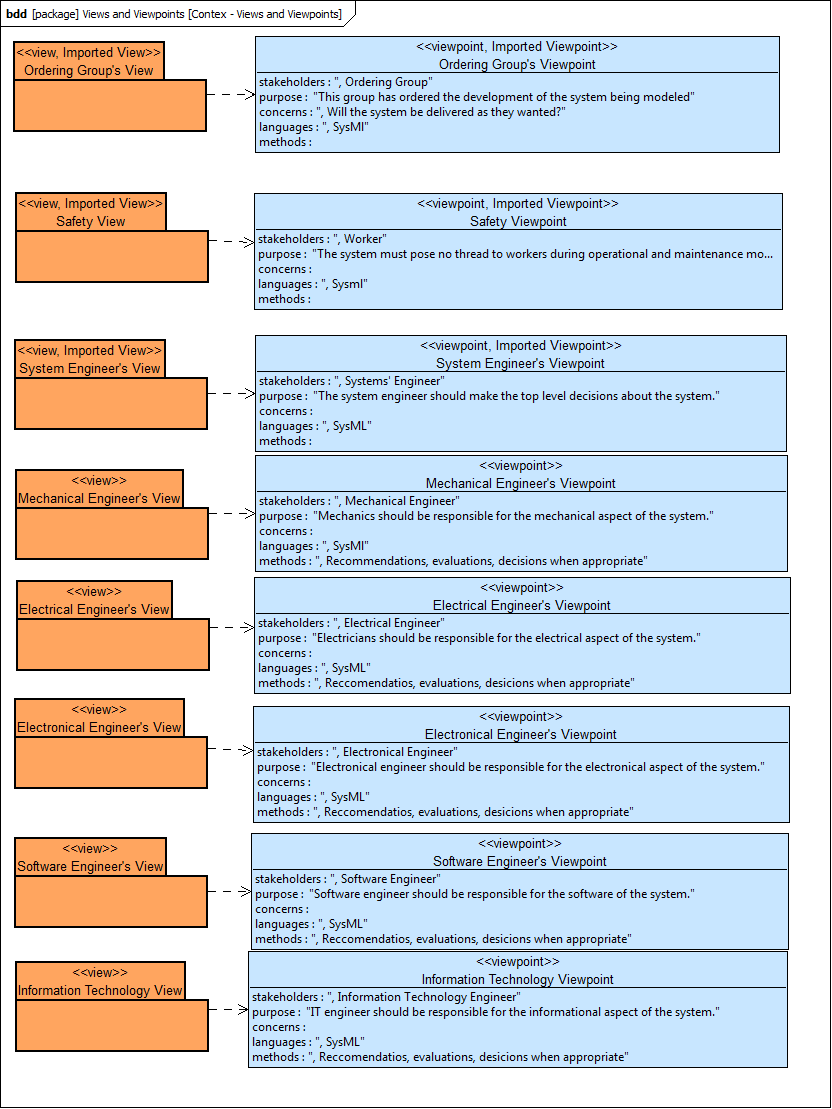
\includegraphics[scale=0.30]{AnalysisModel_Contex-ViewsandViewpoints.png}
					\caption{Οι όψεις του μοντέλου Ανάλυσης}
					\label{φωτ:Οι όψεις του μοντέλου Ανάλυσης}
				\end{figure}
				
				\begin{figure}[hp]
					\centering
					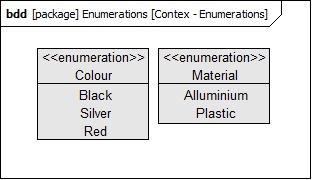
\includegraphics[scale=0.50]{AnalysisModel_Contex-Enumerations.png}
					\caption{Οι "απαριθμήσεις" του μοντέλου Ανάλυσης}
					\label{φωτ:Οι "απαριθμήσεις" του μοντέλου Ανάλυσης}
				\end{figure}		

%%%%%%%%%%%%%%%%%%%%%%%%%%%%%%%%%%%%%%%%%%%%%%%%%%%%%%%%%%%%%
%%%%%%%%%%%%%%		   							Υποενότητα		   					   %%%%%%%%%%%%%%%%%%%%			
			\FloatBarrier
			\subsection{Πακέτο απαιτήσεων\index{πακέτο!απαιτήσεις}\index{απαιτήσεις!πακέτο} - Requirements package\index{requirements!package}\index{package!requirements}}

			\clearpage
			\begin{figure}[hp]
					\centering
					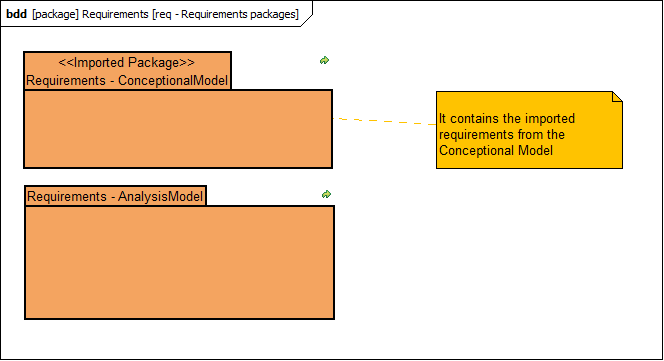
\includegraphics[scale=0.30]{AnalysisModel_req-Requirementspackages.png}
					\caption{Η δομή των απαιτήσεων του μοντέλου Ανάλυσης}
					\label{φωτ:Η δομή των απαιτήσεων του μοντέλου Ανάλυσης}
			\end{figure}
			
			\begin{figure}[hp]
					\centering
					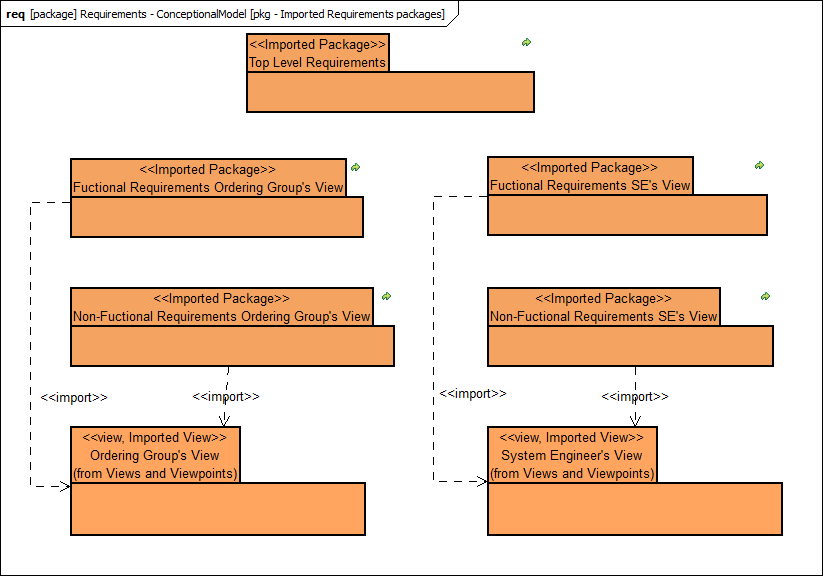
\includegraphics[scale=0.30]{AnalysisModel_pkg-ImportedRequirementspackages.png}
					\caption{Η δομή των απαιτήσεων του μοντέλου Ανάλυσης που έχουν εισαχθεί από το μοντέλο Σύλληψης}
					\label{φωτ:Η δομή των απαιτήσεων του μοντέλου Ανάλυσης που έχουν εισαχθεί από το μοντέλο Σύλληψης}
			\end{figure}
			
			\begin{figure}[hp]
					\centering
					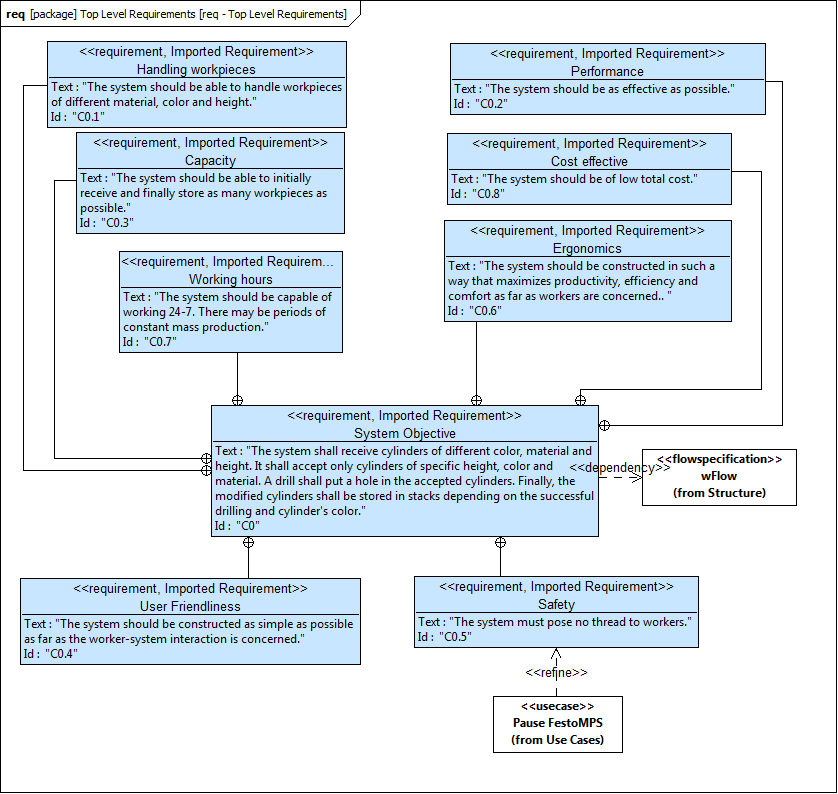
\includegraphics[scale=0.45]{AnalysisModel_req-TopLevelRequirements.png}
					\caption{Οι γενικές απαιτήσεις του μοντέλου Ανάλυσης που έχουν εισαχθεί από το μοντέλο σύλληψης}
					\label{φωτ:Οι γενικές απαιτήσεις του μοντέλου Ανάλυσης που έχουν εισαχθεί από το μοντέλο σύλληψης}
			\end{figure}
				
			\begin{figure}[hp]
					\centering
					\includegraphics[scale=0.45]{AnalysisModel_req-FuctionalRequirementsOrderingGroupsView.png}
					\caption{Οι λειτουργικές απαιτήσεις της ομάδας παραγγελίας στο μοντέλο Ανάλυσης που έχουν εισαχθεί από το μοντέλο Σύλληψης}
					\label{φωτ:Οι λειτουργικές απαιτήσεις της ομάδας παραγγελίας στο μοντέλο Ανάλυσης που έχουν εισαχθεί από το μοντέλο Σύλληψης}
			\end{figure}
				
			\begin{figure}[hp]
					\centering
					\includegraphics[scale=0.45]{AnalysisModel_req-Non-FuctionalRequirementsOrderingGroupsView.png}
					\caption{Οι λοιπές απαιτήσεις της ομάδας παραγγελίας στο μοντέλο Ανάλυσης που έχουν εισαχθεί από το μοντέλο Σύλληψης}
				\label{φωτ:Οι λοιπές απαιτήσεις της ομάδας παραγγελίας στο μοντέλο Ανάλυσης που έχουν εισαχθεί από το μοντέλο Σύλληψης}
			\end{figure}
				
			\begin{figure}[hp]
					\centering
					\includegraphics[scale=0.45]{AnalysisModel_req-FuctionalRequirementsSEsView.png}
					\caption{Οι λειτουργικές απαιτήσεις του μηχανικού συστημάτων στο μοντέλο Ανάλυσης που έχουν εισαχθεί από το μοντέλο Σύλληψης}
					\label{φωτ:Οι λειτουργικές απαιτήσεις του μηχανικού συστημάτων στο μοντέλο Ανάλυσης που έχουν εισαχθεί από το μοντέλο Σύλληψης}
			\end{figure}
				
			\begin{figure}[hp]
					\centering
					\includegraphics[scale=0.30]{AnalysisModel_req-Non-FuctionalRequirementsSEsView.png}
					\caption{Οι λοιπές απαιτήσεις του μηχανικού συστημάτων στο μοντέλο Ανάλυσης που έχουν εισαχθεί από το μοντέλο Σύλληψης}
					\label{φωτ:Οι λοιπές απαιτήσεις του μηχανικού συστημάτων στο μοντέλο Ανάλυσης που έχουν εισαχθεί από το μοντέλο Σύλληψης}
			\end{figure}
			
			\begin{figure}[hp]
					\centering
					\includegraphics[scale=0.30]{AnalysisModel_req-StationRequirements(DistributionStation).png}
					\caption{Οι απαιτήσεις του σταθμού διανομής στο μοντέλο Ανάλυσης}
					\label{φωτ:Οι απαιτήσεις του σταθμού διανομής στο μοντέλο Ανάλυσης}
			\end{figure}
			
			\begin{figure}[hp]
					\centering
					\includegraphics[scale=0.30]{AnalysisModel_req-StationRequirements(TestingStation).png}
					\caption{Οι απαιτήσεις του σταθμού ελέγχου στο μοντέλο Ανάλυσης}
					\label{φωτ:Οι απαιτήσεις του σταθμού ελέγχου στο μοντέλο Ανάλυσης}
			\end{figure}
			
			\begin{figure}[hp]
					\centering
					\includegraphics[scale=0.30]{AnalysisModel_req-StationRequirements(ProcessingStation).png}
					\caption{Οι απαιτήσεις του σταθμού επεξεργασίας στο μοντέλο Ανάλυσης}
					\label{φωτ:Οι απαιτήσεις του σταθμού επεξεργασίας στο μοντέλο Ανάλυσης}
			\end{figure}
			
			\begin{figure}[hp]
					\centering
					\includegraphics[scale=0.30]{AnalysisModel_req-StationRequirements(WarehousingStation).png}
					\caption{Οι απαιτήσεις του σταθμού αποθήκευσης στο μοντέλο Ανάλυσης}
					\label{φωτ:Οι απαιτήσεις του σταθμού αποθήκευσης στο μοντέλο Ανάλυσης}
			\end{figure}
			
			\begin{figure}[hp]
					\centering
					\includegraphics[scale=0.20]{AnalysisModel_req-Satisfaction(ConceptionalModelsRequirements).png}
					\caption{Η πλήρωση των απαιτήσεων του μοντέλου Σύλληψης}
					\label{φωτ:Η πλήρωση των απαιτήσεων του μοντέλου Σύλληψης}
			\end{figure}
			
			\begin{figure}[hp]
					\centering
					\includegraphics[scale=0.30]{AnalysisModel_req-Satisfaction(DistributionStationsRequirements).png}
					\caption{Η πλήρωση των απαιτήσεων του σταθμού διανομής στο μοντέλο Ανάλυσης}
					\label{φωτ:Η πλήρωση των απαιτήσεων του σταθμού διανομής στο μοντέλο Ανάλυσης}
			\end{figure}
			
			\begin{figure}[hp]
					\centering
					\includegraphics[scale=0.30]{AnalysisModel_req-Satisfaction(TestingStationsRequirements).png}
					\caption{Η πλήρωση των απαιτήσεων του σταθμού ελέγχου στο μοντέλο Ανάλυσης}
					\label{φωτ:Η πλήρωση των απαιτήσεων του σταθμού ελέγχου στο μοντέλο Ανάλυσης}
			\end{figure}
			
			\begin{figure}[hp]
					\centering
					\includegraphics[scale=0.30]{AnalysisModel_req-Satisfaction(ProcessingStationsRequirements).png}
					\caption{Η πλήρωση των απαιτήσεων του σταθμού επεξεργασίας στο μοντέλο Ανάλυσης}
					\label{φωτ:Η πλήρωση των απαιτήσεων του σταθμού επεξεργασίας στο μοντέλο Ανάλυσης}
			\end{figure}
			
			\begin{figure}[hp]
					\centering
					\includegraphics[scale=0.30]{AnalysisModel_req-Satisfaction(WarehousingStationsRequirements).png}
					\caption{Η πλήρωση των απαιτήσεων του σταθμού αποθήκευσης στο μοντέλο Ανάλυσης}
					\label{φωτ:Η πλήρωση των απαιτήσεων του σταθμού αποθήκευσης στο μοντέλο Ανάλυσης}
			\end{figure}
			
			\begin{figure}[hp]
					\centering
					\includegraphics[scale=0.30]{AnalysisModel_req-StationRequirements(CentralControlStation).png}
					\caption{Η πλήρωση των απαιτήσεων του σταθμού κεντρικού ελέγχου στο μοντέλο Ανάλυσης}
					\label{φωτ:Η πλήρωση των απαιτήσεων του σταθμού κεντρικού ελέγχου στο μοντέλο Ανάλυσης}
			\end{figure}

%%%%%%%%%%%%%%%%%%%%%%%%%%%%%%%%%%%%%%%%%%%%%%%%%%%%%%%%%%%%%
%%%%%%%%%%%%%%		   							Υποενότητα		   					   %%%%%%%%%%%%%%%%%%%%			
			\FloatBarrier
			\subsection{Πακέτο δομής\index{πακέτο!δομής}\index{δομή!πακέτο} - Structure package\index{structure!package}\index{package!structure}}

			\clearpage
			\begin{figure}[hp]
					\centering
					\includegraphics[scale=0.30]{AnalysisModel_bdd-HierarchyofTopLevelBlocks.png}
					\caption{Η ιεραρχική διάρθρωση των βασικών δομικών στοιχείων στο μοντέλο Ανάλυσης}
					\label{φωτ:Η ιεραρχική διάρθρωση των βασικών δομικών στοιχείων στο μοντέλο Ανάλυσης}
			\end{figure}
			
			\begin{figure}[hp]
					\centering
					\includegraphics[scale=0.30]{AnalysisModel_bdd-Hierarchyof2ndLevelBlocks.png}
					\caption{Η ιεραρχική διάρθρωση των δευτερευόντων δομικών στοιχείων στο μοντέλο Ανάλυσης}
					\label{φωτ:Η ιεραρχική διάρθρωση των δευτερευόντων δομικών στοιχείων στο μοντέλο Ανάλυσης}
			\end{figure}
			
			\begin{figure}[hp]
					\centering
					\includegraphics[scale=0.30]{AnalysisModel_bdd-FlowSpesifications.png}
					\caption{Οι τεκμηριώσεις των ροών στο μοντέλο Ανάλυσης}
					\label{φωτ:Οι τεκμηριώσεις των ροών στο μοντέλο Ανάλυσης}
			\end{figure}
			
			\begin{figure}[hp]
					\centering
					\includegraphics[scale=0.30]{AnalysisModel_bdd-Interfaces.png}
					\caption{Οι τεκμηριώσεις των διεπαφών στο μοντέλο Ανάλυσης}
					\label{φωτ:Οι τεκμηριώσεις των διεπαφών στο μοντέλο Ανάλυσης}
			\end{figure}
			
			\begin{figure}[hp]
					\centering
					\includegraphics[scale=0.30]{AnalysisModel_bdd-TopLevelStructureofFestoMPS.png}
					\caption{To bdd του Festo Mps στο μοντέλο Ανάλυσης}
					\label{φωτ:To bdd του Festo Mps στο μοντέλο Ανάλυσης}
			\end{figure}
			
			\begin{figure}[hp]
					\centering
					\includegraphics[scale=0.30]{AnalysisModel_ibd-FestoMPSconnectionsinvolvingworkpieces.png}
					\caption{To ibd του Festo MPS αναφερόμενο στις πρώτες ύλες στο μοντέλο Ανάλυσης}
					\label{φωτ:To ibd του Festo MPS αναφερόμενο στις πρώτες ύλες στο μοντέλο Ανάλυσης}
			\end{figure}
			
			\begin{figure}[hp]
					\centering
					\includegraphics[scale=0.30]{AnalysisModel_ibd-FestoMPSconnectionsinvolvingcentralcontrolstructuralconnections.png}
					\caption{To ibd του Festo MPS αναφερόμενο στις γραμμές ελέγχου στο μοντέλο Ανάλυσης}
					\label{φωτ:To ibd του Festo MPS αναφερόμενο στις γραμμές ελέγχου στο μοντέλο Ανάλυσης}
			\end{figure}
			
			\begin{figure}[hp]
					\centering
					\includegraphics[scale=0.30]{AnalysisModel_ibd-FestoMPSconnectionsinvolvingcentralcontrolinterfaces.png}
					\caption{To ibd του Festo MPS αναφερόμενο στις διεπαφές στο μοντέλο Ανάλυσης}
					\label{φωτ:To ibd του Festo MPS αναφερόμενο στις διεπαφές στο μοντέλο Ανάλυσης}
			\end{figure}
			
			\begin{figure}[hp]
					\centering
					\includegraphics[scale=0.30]{AnalysisModel_ibd-FestoMPSconnectionsinvolvingenergy.png}
					\caption{To ibd του Festo MPS αναφερόμενο στην ενέργεια στο μοντέλο Ανάλυσης}
					\label{φωτ:To ibd του Festo MPS αναφερόμενο στην ενέργεια στο μοντέλο Ανάλυσης}
			\end{figure}
			
			\begin{figure}[hp]
					\centering
					\includegraphics[scale=0.30]{AnalysisModel_bdd-DistributionStationsStructure.png}
					\caption{To bdd του σταθμού διανομής στο μοντέλο Ανάλυσης}
					\label{φωτ:To bdd του σταθμού διανομής στο μοντέλο Ανάλυσης}
			\end{figure}
			
			\begin{figure}[hp]
					\centering
					\includegraphics[scale=0.30]{AnalysisModel_ibd-DistributionStation.png}
					\caption{To ibd του σταθμού διανομής στο μοντέλο Ανάλυσης}
					\label{φωτ:To ibd του σταθμού διανομής στο μοντέλο Ανάλυσης}
			\end{figure}
			
			\begin{figure}[hp]
					\centering
					\includegraphics[scale=0.30]{AnalysisModel_bdd-TestingStationsStructure.png}
					\caption{To bdd του σταθμού ελέγχου στο μοντέλο Ανάλυσης}
					\label{φωτ:To bdd του σταθμού ελέγχου Festo Mps στο μοντέλο Ανάλυσης}
			\end{figure}
			
			\begin{figure}[hp]
					\centering
					\includegraphics[scale=0.30]{AnalysisModel_ibd-TestingStationconnectionsinvolvingworkpieces.png}
					\caption{To ibd του σταθμού ελέγχου αναφερόμενο στις πρώτες ύλες στο μοντέλο Ανάλυσης}
					\label{φωτ:To ibd του σταθμού ελέγχου αναφερόμενο στις πρώτες ύλες στο μοντέλο Ανάλυσης}
			\end{figure}
			
			\begin{figure}[hp]
					\centering
					\includegraphics[scale=0.30]{AnalysisModel_ibd-TestingStationconnectionsinvolvingcontrol.png}
					\caption{To ibd του σταθμού ελέγχου αναφερόμενο στον έλεγχο στο μοντέλο Ανάλυσης}
					\label{φωτ:To ibd του σταθμού ελέγχου αναφερόμενο στον έλεγχο στο μοντέλο Ανάλυσης}
			\end{figure}
			
			\begin{figure}[hp]
					\centering
					\includegraphics[scale=0.30]{AnalysisModel_ibd-RecognizingModule.png}
					\caption{To ibd της μονάδας αναγνώρισης στο μοντέλο Ανάλυσης}
					\label{φωτ:To ibd της μονάδας αναγνώρισης στο μοντέλο Ανάλυσης}
			\end{figure}
			
			\begin{figure}[hp]
					\centering
					\includegraphics[scale=0.30]{AnalysisModel_bdd-ProcessingStationsStructure.png}
					\caption{To bdd του σταθμού επεξεργασίας στο μοντέλο Ανάλυσης}
					\label{φωτ:To bdd του σταθμού επεξεργασίας στο μοντέλο Ανάλυσης}
			\end{figure}
			
			\begin{figure}[hp]
					\centering
					\includegraphics[scale=0.30]{AnalysisModel_ibd-ProcessingStation.png}
					\caption{To ibd του σταθμού επεξεργασίας στο μοντέλο Ανάλυσης}
					\label{φωτ:To ibd του σταθμού επεξεργασίας στο μοντέλο Ανάλυσης}
			\end{figure}
			
			\begin{figure}[hp]
					\centering
					\includegraphics[scale=0.50]{AnalysisModel_bdd-WarehouseStationsStructure.png}
					\caption{To bdd του σταθμού αποθήκευσης στο μοντέλο Ανάλυσης}
					\label{φωτ:To bdd του σταθμού αποθήκευσης στο μοντέλο Ανάλυσης}
			\end{figure}
			
			\clearpage
			\begin{figure}[hp]
					\centering
					\includegraphics[scale=0.50]{AnalysisModel_ibd-WarehouseStation.png}
					\caption{To ibd του σταθμού αποθήκευσης στο μοντέλο Ανάλυσης}
					\label{φωτ:To ibd του σταθμού αποθήκευσης στο μοντέλο Ανάλυσης}
			\end{figure}
			
			\begin{figure}[hp]
					\centering
					\includegraphics[scale=0.50]{AnalysisModel_bdd-CentralControlStationsStructure.png}
					\caption{To bdd του σταθμού κεντρικού ελέχου στο μοντέλο Ανάλυσης}
					\label{φωτ:To bdd του σταθμού κεντρικού ελέγχου στο μοντέλο Ανάλυσης}
			\end{figure}
			
			\begin{figure}[hp]
					\centering
					\includegraphics[scale=0.50]{AnalysisModel_ibd-CentralControlStation.png}
					\caption{To ibd του σταθμού κεντρικού ελέγχου στο μοντέλο Ανάλυσης}
					\label{φωτ:To ibd του σταθμού κεντρικού ελέγχου στο μοντέλο Ανάλυσης}
			\end{figure}

%%%%%%%%%%%%%%%%%%%%%%%%%%%%%%%%%%%%%%%%%%%%%%%%%%%%%%%%%%%%%
%%%%%%%%%%%%%%		   							Υποενότητα		   					   %%%%%%%%%%%%%%%%%%%%			
			\FloatBarrier
			\subsection{Πακέτο λειτουργίας\index{πακέτο!λειτουργίας}\index{λειτουργία!πακέτο} - Behaviour package\index{behavioul!package}\index{package!behaviour}}

			\clearpage
			\begin{figure}[hp]
					\centering
					\includegraphics[scale=0.30]{AnalysisModel_uc-TopLevelUseCases.png}
					\caption{Οι περιπτώσεις χρήσεις του Festo MPS στο μοντέλο Ανάλυσης}
					\label{φωτ:Οι περιπτώσεις χρήσεις του Festo MPS στο μοντέλο Ανάλυσης}
			\end{figure}
			
			\begin{figure}[hp]
					\centering
					\includegraphics[scale=0.30]{AnalysisModel_stm-FestoMpsTopLevelStates.png}
					\caption{Το διάγραμμα καταστάσεων του Festo MPS στο μοντέλο Ανάλυσης}
					\label{φωτ:Το διάγραμμα καταστάσεων του Festo MPS στο μοντέλο Ανάλυσης}
			\end{figure}
			
			\begin{figure}[hp]
					\centering
					\includegraphics[scale=0.30]{AnalysisModel_seq-FestoMpsTopLevelSequence.png}
					\caption{Το διάγραμμα ακολουθίας του Festo MPS στο μοντέλο Ανάλυσης}
					\label{φωτ:Το διάγραμμα ακολουθίας του Festo MPS στο μοντέλο Ανάλυσης}
			\end{figure}
			
			\begin{figure}[hp]
					\centering
					\includegraphics[scale=0.30]{AnalysisModel_seq-PowerOn.png}
					\caption{Το διάγραμμα ακολουθίας για την ενεργοποίηση του Festo MPS στο μοντέλο Ανάλυσης}
					\label{φωτ:Το διάγραμμα ακολουθίας για την ενεργοποίηση του Festo MPS στο μοντέλο Ανάλυσης}
			\end{figure}
			
			\begin{figure}[hp]
					\centering
					\includegraphics[scale=0.30]{AnalysisModel_seq-InitializeSystem.png}
					\caption{Το διάγραμμα ακολουθίας για την αρχικοποίηση του Festo MPS στο μοντέλο Ανάλυσης}
					\label{φωτ:Το διάγραμμα ακολουθίας για την αρχικοποίηση του Festo MPS στο μοντέλο Ανάλυσης}
			\end{figure}
			
			\begin{figure}[hp]
					\centering
					\includegraphics[scale=0.30]{AnalysisModel_seq-TerminateSystem.png}
					\caption{Το διάγραμμα ακολουθίας για τον τερματισμό εκκίνηση του Festo MPS στο μοντέλο Ανάλυσης}
					\label{φωτ:Το διάγραμμα ακολουθίας για τον τερματισμό του Festo MPS στο μοντέλο Ανάλυσης}
			\end{figure}
			
			\begin{figure}[hp]
					\centering
					\includegraphics[scale=0.30]{AnalysisModel_seq-PowerOff.png}
					\caption{Το διάγραμμα ακολουθίας για την απενεργοποίηση του Festo MPS στο μοντέλο Ανάλυσης}
					\label{φωτ:Το διάγραμμα ακολουθίας για την απενεργοποίηση του Festo MPS στο μοντέλο Ανάλυσης}
			\end{figure}
			
			\begin{figure}[hp]
					\centering
					\includegraphics[scale=0.30]{AnalysisModel_uc-DistributionStationsUseCases.png}
					\caption{Οι περιπτώσεις χρήσεις του σταθμού διανομής στο μοντέλο Ανάλυσης}
					\label{φωτ:Οι περιπτώσεις χρήσεις του σταθμού διανομής στο μοντέλο Ανάλυσης}
			\end{figure}
			
			\begin{figure}[hp]
					\centering
					\includegraphics[scale=0.30]{AnalysisModel_seq-DistributionStation(normalprocess).png}
					\caption{Το διάγραμμα ακολουθίας του σταθμού διανομής στο μοντέλο Ανάλυσης}
					\label{φωτ:Το διάγραμμα ακολουθίας του σταθμού διανομής στο μοντέλο Ανάλυσης}
			\end{figure}

			\begin{figure}[hp]
					\centering
					\includegraphics[scale=0.30]{AnalysisModel_uc-TestingStationsUseCases.png}
					\caption{Οι περιπτώσεις χρήσεις του σταθμού ελέγχου στο μοντέλο Ανάλυσης}
					\label{φωτ:Οι περιπτώσεις χρήσεις του σταθμού ελέγχου στο μοντέλο Ανάλυσης}
			\end{figure}
			
			\begin{figure}[hp]
					\centering
					\includegraphics[scale=0.30]{AnalysisModel_stm-TestingStation(Testingstate).png}
					\caption{Το διάγραμμα καταστάσεων του σταθμού ελέγχου στο μοντέλο Ανάλυσης}
					\label{φωτ:Το διάγραμμα καταστάσεων του σταθμού ελέγχου στο μοντέλο Ανάλυσης}
			\end{figure}
			
			\begin{figure}[hp]
					\centering
					\includegraphics[scale=0.30]{AnalysisModel_seq-TestingStation(normalprocess).png}
					\caption{Το διάγραμμα ακολουθίας του σταθμού ελέγχου στο μοντέλο Ανάλυσης}
					\label{φωτ:Το διάγραμμα ακολουθίας του σταθμού ελέγχου στο μοντέλο Ανάλυσης}
			\end{figure}
			
			\begin{figure}[hp]
					\centering
					\includegraphics[scale=0.30]{AnalysisModel_uc-ProcessingStationsUseCases.png}
					\caption{Οι περιπτώσεις χρήσεις του σταθμού επεξεργασίας στο μοντέλο Ανάλυσης}
					\label{φωτ:Οι περιπτώσεις χρήσεις του σταθμού επεξεργασίας στο μοντέλο Ανάλυσης}
			\end{figure}
			
			\begin{figure}[hp]
					\centering
					\includegraphics[scale=0.30]{AnalysisModel_stm-ProcessingStation(Processingstate).png}
					\caption{Το διάγραμμα καταστάσεων του σταθμού επεξεργασίας στο μοντέλο Ανάλυσης}
					\label{φωτ:Το διάγραμμα καταστάσεων του σταθμού επεξεργασίας στο μοντέλο Ανάλυσης}
			\end{figure}
			
			\begin{figure}[hp]
					\centering
					\includegraphics[scale=0.30]{AnalysisModel_seq-ProcessingStation(normalprocess).png}
					\caption{Το διάγραμμα ακολουθίας του σταθμού επεξεργασίας στο μοντέλο Ανάλυσης}
					\label{φωτ:Το διάγραμμα ακολουθίας του σταθμού επεξεργασίας στο μοντέλο Ανάλυσης}
			\end{figure}
			
			\begin{figure}[hp]
					\centering
					\includegraphics[scale=0.30]{AnalysisModel_uc-WarehousingStationsUseCases.png}
					\caption{Οι περιπτώσεις χρήσεις του σταθμού αποθήκευσης στο μοντέλο Ανάλυσης}
					\label{φωτ:Οι περιπτώσεις χρήσεις του σταθμού αποθήκευσης στο μοντέλο Ανάλυσης}
			\end{figure}

			\begin{figure}[hp]
					\centering
					\includegraphics[scale=0.30]{AnalysisModel_seq-WarehousingStation(normalprocess).png}
					\caption{Το διάγραμμα ακολουθίας του σταθμού αποθήκευσης στο μοντέλο Ανάλυσης}
					\label{φωτ:Το διάγραμμα ακολουθίας του σταθμού αποθήκευσης στο μοντέλο Ανάλυσης}
			\end{figure}
			
			\begin{figure}[hp]
					\centering
					\includegraphics[scale=0.30]{AnalysisModel_uc-CentralEnergyStationsUseCases.png}
					\caption{Οι περιπτώσεις χρήσεις του σταθμού ενέργειας στο μοντέλο Ανάλυσης}
					\label{φωτ:Οι περιπτώσεις χρήσεις του σταθμού ενέργειας στο μοντέλο Ανάλυσης}
			\end{figure}
			
			\clearpage
			\begin{figure}[hp]
					\centering
					\includegraphics[scale=0.30]{AnalysisModel_uc-CentralControlStationsUseCases.png}
					\caption{Οι περιπτώσεις χρήσεις του σταθμού κεντρικού ελέγχου στο μοντέλο Ανάλυσης}
					\label{φωτ:Οι περιπτώσεις χρήσεις του σταθμού κεντρικού ελέγχου στο μοντέλο Ανάλυσης}
			\end{figure}
		
%%%%%%%%%%%%%%%%%%%%%%%%%%%%%%%%%%%%%%%%%%%%%%%%%%%%%%%%%%%%%
%%%%%%%%%%%%%%		   								 Ενότητα		   					   %%%%%%%%%%%%%%%%%%%%
%%%%%%%%%%%%%%%%%%%%%%%%%%%%%%%%%%%%%%%%%%%%%%%%%%%%%%%%%%%%%			
		\FloatBarrier
		\section{Μοντέλο Υλοποίησης\index{μοντέλο!υλοποίησης}  -Design Model\index{model!design}}
		
		%%%%%%%%%%%%%%%%%%%%%%%%%%%%%%%%%%%%%%%%%%%%%%%%%%%%%%%%%%%%%
%%%%%%%%%%%%%%		   							Υποενότητα		   					   %%%%%%%%%%%%%%%%%%%%
			\FloatBarrier
			\subsection{Χώρος υλοποίησης συστήματος\index{χώρος υλοποίησης} - Contex\index{contex}}
			
				\clearpage
				\begin{figure}[hp]
					\centering
					\includegraphics[scale=0.45]{DesignModel_DesignModel.png}
					\caption{Η δομή του μοντέλου Υλοποίησης}
					\label{φωτ:Η δομή του μοντέλου Υλοποίησης}
				\end{figure}
				
				\begin{figure}[hp]
					\centering
					\includegraphics[scale=0.45]{DesignModel_Contex-FestoMPSDomain.png}
					\caption{Ο χώρος υλοποίησης του μοντέλου Υλοποίησης}
					\label{φωτ:Ο χώρος υλοποίησης του μοντέλου Υλοποίησης}
				\end{figure}
				
				\begin{figure}[hp]
					\centering
					\includegraphics[scale=0.50]{DesignModel_Contex-Actors.png}
					\caption{Οι ρόλοι του μοντέλου Υλοποίησης}
					\label{φωτ:Οι ρόλοι του μοντέλου Υλοποίησης}
				\end{figure}
				
				\begin{figure}[hp]
					\centering
					\includegraphics[scale=0.30]{DesignModel_Contex-ViewsandViewpoints.png}
					\caption{Οι όψεις του μοντέλου Υλοποίησης}
					\label{φωτ:Οι όψεις του μοντέλου Υλοποίησης}
				\end{figure}
				
				\begin{figure}[hp]
					\centering
					\includegraphics[scale=0.50]{DesignModel_Contex-OtherDefinitions.png}
					\caption{Τα λοιπά στοιχεία του μοντέλου Υλοποίησης}
					\label{φωτ:Τα λοιπά στοιχεία του μοντέλου Υλοποίησης}
				\end{figure}
				
				\begin{figure}[hp]
					\centering
					\includegraphics[scale=0.50]{DesignModel_Contex-Enumerations.png}
					\caption{Οι "απαριθμήσεις" του μοντέλου Υλοποίησης}
					\label{φωτ:Οι "απαριθμήσεις" του μοντέλου Υλοποίησης}
				\end{figure}
				
				\begin{figure}[hp]
					\centering
					\includegraphics[scale=0.50]{DesignModel_Contex-FlowSpecifications.png}
					\caption{Η τεκμηρίωση των ροών του μοντέλου Υλοποίησης}
					\label{φωτ:Η τεκμηρίωση των ροών του μοντέλου Υλοποίησης}
				\end{figure}
				
				\begin{figure}[hp]
					\centering
					\includegraphics[scale=0.50]{DesignModel_Contex-Values.png}
					\caption{Οι κατηγορίες των υπό μέτρηση μεγεθών του μοντέλου Υλοποίησης}
					\label{φωτ:Οι κατηγορίες των υπό μέτρηση μεγεθών του μοντέλου Υλοποίησης}
				\end{figure}
				
				\begin{figure}[hp]
					\centering
					\includegraphics[scale=0.30]{DesignModel_Contex-Units.png}
					\caption{Οι μονάδες μέτρησης του μοντέλου Υλοποίησης}
					\label{φωτ:Οι μονάδες μέτρησης του μοντέλου Υλοποίησης}
				\end{figure}
				
				\begin{figure}[hp]
					\centering
					\includegraphics[scale=0.50]{DesignModel_Contex-Dimensions.png}
					\caption{Τα υπό μέτρηση μεγέθη του μοντέλου Υλοποίησης}
					\label{φωτ:Τα υπό μέτρηση μεγέθη του μοντέλου Υλοποίησης}
				\end{figure}
				
				\begin{figure}[hp]
					\centering
					\includegraphics[scale=0.50]{DesignModel_Contex-Workpieces.png}
					\caption{Το bdd των πρώτων υλών στο μοντέλο Υλοποίησης}
					\label{φωτ:Το bdd των πρώτων υλών στο μοντέλο Υλοποίησης}
				\end{figure}
				
				\begin{figure}[hp]
					\centering
					\includegraphics[scale=0.50]{DesignModel_Contex-Parts(UnitsClassification).png}
					\caption{Η κατάταξη των συκευών στο μοντέλο Υλοποίησης}
					\label{φωτ:Η κατάταξη των συκευών στο μοντέλο Υλοποίησης}
				\end{figure}
				
				\begin{figure}[hp]
					\centering
					\includegraphics[scale=0.30]{DesignModel_Contex-Parts(SensorUnits).png}
					\caption{Η ιεραρχική διάρθρωση των αισθητήρων στο μοντέλο Υλοποίησης}
					\label{φωτ:Η ιεραρχική διάρθρωση των αισθητήρων στο μοντέλο Υλοποίησης}
				\end{figure}
				
				\begin{figure}[hp]
					\centering
					\includegraphics[scale=0.50]{DesignModel_Contex-Parts(Sensors)[AnalogueSensors].png}
					\caption{Οι αναλογικοί αισθητήρες του μοντέλου Υλοποίησης}
					\label{φωτ:Οι αναλογικοί αισθητήρες του μοντέλου Υλοποίησης}
				\end{figure}
				
				\begin{figure}[hp]
					\centering
					\includegraphics[scale=0.50]{DesignModel_Contex-Parts(Sensors)[MagneticSensors].png}
					\caption{Οι μαγνητικοί αισθητήρες του μοντέλου Υλοποίησης}
					\label{φωτ:Οι μαγνητικοί αισθητήρες του μοντέλου Υλοποίησης}
				\end{figure}
				
				\begin{figure}[hp]
					\centering
					\includegraphics[scale=0.50]{DesignModel_Contex-Parts(Sensors)[MicroSwitch].png}
					\caption{Οι τερματικοί αισθητήρες του μοντέλου Υλοποίησης}
					\label{φωτ:Οι τερματικοί αισθητήρες του μοντέλου Υλοποίησης}
				\end{figure}
				
				\begin{figure}[hp]
					\centering
					\includegraphics[scale=0.50]{DesignModel_Contex-Parts(Sensors)[InductiveSensor].png}
					\caption{Οι επαγωγικοί αισθητήρες του μοντέλου Υλοποίησης}
					\label{φωτ:Οι επαγωγικοί αισθητήρες του μοντέλου Υλοποίησης}
				\end{figure}
				
				\begin{figure}[hp]
					\centering
					\includegraphics[scale=0.50]{DesignModel_Contex-Parts(Sensors)[CapacitiveSensors].png}
					\caption{Οι χωρητικοί αισθητήρες του μοντέλου Υλοποίησης}
					\label{φωτ:Οι χωρητικοί αισθητήρες του μοντέλου Υλοποίησης}
				\end{figure}
				
				\clearpage
				\begin{figure}[hp]
					\centering
					\includegraphics[scale=0.50]{DesignModel_Contex-Parts(Sensors)[VacuumSwitch].png}
					\caption{Οι αισθητήρες κενού του μοντέλου Υλοποίησης}
					\label{φωτ:Οι αισθητήρες κενού του μοντέλου Υλοποίησης}
				\end{figure}
				
				\begin{figure}[hp]
					\centering
					\includegraphics[scale=0.50]{DesignModel_Contex-Parts(Sensors)[Retro-reflectiveSensors].png}
					\caption{Οι αισθητήρες ανάκλασης του μοντέλου Υλοποίησης}
					\label{φωτ:Οι αισθητήρες ανάκλασης του μοντέλου Υλοποίησης}
				\end{figure}
				
				\begin{figure}[hp]
					\centering
					\includegraphics[scale=0.50]{DesignModel_Contex-Parts(Sensors)[Through-beamSensor].png}
					\caption{Οι αισθητήρες φωτοκύτταρου του μοντέλου Υλοποίησης}
					\label{φωτ:Οι αισθητήρες φωτοκύτταρου του μοντέλου Υλοποίησης}
				\end{figure}
				
				\begin{figure}[hp]
					\centering
					\includegraphics[scale=0.50]{DesignModel_Contex-Parts(Sensors)[DiffuseSensors].png}
					\caption{Οι αισθητήρες διάχυσης του μοντέλου Υλοποίησης}
					\label{φωτ:Οι αισθητήρες διάχυσης του μοντέλου Υλοποίησης}
				\end{figure}
				
				\begin{figure}[hp]
					\centering
					\includegraphics[scale=0.50]{DesignModel_Contex-Parts(ActuatorUnits).png}
					\caption{Η ιεραρχική διάρθρωση των ενεργοποιητών στο μοντέλο Υλοποίησης}
					\label{φωτ:Η ιεραρχική διάρθρωση των ενεργοποιητών στο μοντέλο Υλοποίησης}
				\end{figure}
				
				\begin{figure}[hp]
					\centering
					\includegraphics[scale=0.50]{DesignModel_Contex-Parts(ActuatorUnits)[Double-actingCylinder].png}
					\caption{Οι πνευματικοί κύλινδροι του μοντέλου Υλοποίησης}
					\label{φωτ:Οι πνευματικοί κύλινδροι του μοντέλου Υλοποίησης}
				\end{figure}
				
				\begin{figure}[hp]
					\centering
					\includegraphics[scale=0.50]{DesignModel_Contex-Parts(ActuatorUnits)[ValveNon-Return].png}
					\caption{Οι βαλβίδες χωρίς επιστροφή του μοντέλου Υλοποίησης}
					\label{φωτ:Οι βαλβίδες χωρίς επιστροφή του μοντέλου Υλοποίησης}
				\end{figure}
				
				\begin{figure}[hp]
					\centering
					\includegraphics[scale=0.50]{DesignModel_Contex-Parts(ActuatorUnits)[Valve1way].png}
					\caption{Οι βαλβίδες μίας κατεύθυνσης του μοντέλου Υλοποίησης}
					\label{φωτ:Οι βαλβίδες μίας κατεύθυνσης του μοντέλου Υλοποίησης}
				\end{figure}
				
				\begin{figure}[hp]
					\centering
					\includegraphics[scale=0.50]{DesignModel_Contex-Parts(ActuatorUnits)[Valve5-3Way].png}
					\caption{Οι βαλβίδες 5/3 του μοντέλου Υλοποίησης}
					\label{φωτ:Οι βαλβίδες 5/3 του μοντέλου Υλοποίησης}
				\end{figure}
				
				\begin{figure}[hp]
					\centering
					\includegraphics[scale=0.50]{DesignModel_Contex-Parts(ActuatorUnits)[Valve5-2way].png}
					\caption{Οι βαλβίδες 5/2 του μοντέλου Υλοποίησης}
					\label{φωτ:Οι βαλβίδες 5/2 του μοντέλου Υλοποίησης}
				\end{figure}
				
				\begin{figure}[hp]
					\centering
					\includegraphics[scale=0.50]{DesignModel_Contex-Parts(ActuatorUnits)[ElectricRelays].png}
					\caption{Τα ηλεκτρικά ρελέ του μοντέλου Υλοποίησης}
					\label{φωτ:Τα ηλεκτρικά ρελέ του μοντέλου Υλοποίησης}
				\end{figure}
				
				\begin{figure}[hp]
					\centering
					\includegraphics[scale=0.50]{DesignModel_Contex-Parts(ActuatorUnits)[ElectricValveControllers].png}
					\caption{Οι ελεγκτές ηλεκτρικών βαλβίδων του μοντέλου Υλοποίησης}
					\label{φωτ:Οι ελεγκτές ηλεκτρικών βαλβίδων του μοντέλου Υλοποίησης}
				\end{figure}
				
				\begin{figure}[hp]
					\centering
					\includegraphics[scale=0.50]{DesignModel_Contex-Parts(ConveyorUnits).png}
					\caption{Η ιεραρχική διάρθρωση των μονάδων μεταφοράς στο μοντέλο Υλοποίησης}
					\label{φωτ:Η ιεραρχική διάρθρωση των μονάδων μεταφοράς στο μοντέλο Υλοποίησης}
				\end{figure}
				
				\begin{figure}[hp]
					\centering
					\includegraphics[scale=0.50]{DesignModel_Contex-Parts(ConveyorUnits)[SuctionCup(1Axis)].png}
					\caption{Οι μονάδες μεταφοράς με βεντούζα κενού του μοντέλου Υλοποίησης}
					\label{φωτ:Οι μονάδες μεταφοράς με βεντούζα κενού του μοντέλου Υλοποίησης}
				\end{figure}
				
				\begin{figure}[hp]
					\centering
					\includegraphics[scale=0.50]{DesignModel_Contex-Parts(ConveyorUnits)[Grippers(3Axises)].png}
					\caption{Οι μονάδες μεταφοράς με δαγκάνα του μοντέλου Υλοποίησης}
					\label{φωτ:Οι μονάδες μεταφοράς με δαγκάνα του μοντέλου Υλοποίησης}
				\end{figure}
				
				\begin{figure}[hp]
					\centering
					\includegraphics[scale=0.50]{DesignModel_Contex-Parts(ConveyorUnits)[LiftingUnit].png}
					\caption{Οι μονάδες ανύψωσης του μοντέλου Υλοποίησης}
					\label{φωτ:Οι μονάδες ανύψωσης του μοντέλου Υλοποίησης}
				\end{figure}
				
				\begin{figure}[hp]
					\centering
					\includegraphics[scale=0.50]{DesignModel_Contex-Parts(ConveyorUnits)[SlideUnits].png}
					\caption{Οι πλατφόρμες κύλισης του μοντέλου Υλοποίησης}
					\label{φωτ:Οι πλατφόρμες κύλισης του μοντέλου Υλοποίησης}
				\end{figure}
				
				\begin{figure}[hp]
					\centering
					\includegraphics[scale=0.50]{DesignModel_Contex-Parts(ConveyorUnits)[Air-cushionedSlideUnits].png}
					\caption{Οι πλατφόρμες κύλισης με εξομάλυνση αέρα του μοντέλου Υλοποίησης}
					\label{φωτ:Οι πλατφόρμες κύλισης  με εξομάλυνση αέρα του μοντέλου Υλοποίησης}
				\end{figure}
				
				\clearpage
				\begin{figure}[hp]
					\centering
					\includegraphics[scale=0.50]{DesignModel_Contex-Parts(CommunicationUnits).png}
					\caption{Οι συσκευές επικοινωνίας στο μοντέλο Υλοποίησης}
					\label{φωτ:Οι συσκευές επικοινωνίας στο μοντέλο Υλοποίησης}
				\end{figure}

				\begin{figure}[hp]
					\centering
					\includegraphics[scale=0.50]{DesignModel_Contex-Parts(ProcessingUnits).png}
					\caption{Η ιεραρχική διάρθρωση των μονάδων λειτουργίας στο μοντέλο Υλοποίησης}
					\label{φωτ:Η ιεραρχική διάρθρωση των μονάδων λειτουργίας στο μοντέλο Υλοποίησης}
				\end{figure}
				
				\begin{figure}[hp]
					\centering
					\includegraphics[scale=0.50]{DesignModel_Contex-Parts(ProcessingUnits)[DrillingUnits].png}
					\caption{Οι μονάδες διάτρησης του μοντέλου Υλοποίησης}
					\label{φωτ:Οι μονάδες διάτρησης του μοντέλου Υλοποίησης}
				\end{figure}
				
				\begin{figure}[hp]
					\centering
					\includegraphics[scale=0.50]{DesignModel_Contex-Parts(ProcessingUnits)[MeasuringDepthUnits].png}
					\caption{Οι μονάδες μέτρησης βάθους του μοντέλου Υλοποίησης}
					\label{φωτ:Οι μονάδες μέτρησης βάθους του μοντέλου Υλοποίησης}
				\end{figure}
				
				
				\begin{figure}[hp]
					\centering
					\includegraphics[scale=0.50]{DesignModel_Contex-Parts(SoftwareExecutionUnits).png}
					\caption{Η ιεραρχική διάρθρωση των μονάδων λογισμικού στο μοντέλο Υλοποίησης}
					\label{φωτ:Η ιεραρχική διάρθρωση των μονάδων λογισμικού στο μοντέλο Υλοποίησης}
				\end{figure}
				
				\begin{figure}[hp]
					\centering
					\includegraphics[scale=0.50]{DesignModel_Contex-Parts(WarehouseUnits).png}
					\caption{Η ιεραρχική διάρθρωση των μονάδων αποθήκευσης στο μοντέλο Υλοποίησης}
					\label{φωτ:Η ιεραρχική διάρθρωση των μονάδων αποθήκευσης στο μοντέλο Υλοποίησης}
				\end{figure}
				
				\begin{figure}[hp]
					\centering
					\includegraphics[scale=0.30]{DesignModel_Contex-Parts(OtherUnits).png}
					\caption{Η ιεραρχική διάρθρωση των λοιπών μονάδων στο μοντέλο Υλοποίησης}
					\label{φωτ:Η ιεραρχική διάρθρωσητων λοιπών μονάδων στο μοντέλο Υλοποίησης}
				\end{figure}
				
				\begin{figure}[hp]
					\centering
					\includegraphics[scale=0.50]{DesignModel_Contex-Parts(OtherUnits)[Arms].png}
					\caption{Οι βραχίονες στο μοντέλο Υλοποίησης}
					\label{φωτ:Οι βραχίονες στο μοντέλο Υλοποίησης}
				\end{figure}
				
				\begin{figure}[hp]
					\centering
					\includegraphics[scale=0.50]{DesignModel_Contex-Parts(OtherUnits)[MagazineBarrel].png}
					\caption{Οι στοίβες στο μοντέλο Υλοποίησης}
					\label{φωτ:Οι στοίβες στο μοντέλο Υλοποίησης}
				\end{figure}
				
				\begin{figure}[hp]
					\centering
					\includegraphics[scale=0.50]{DesignModel_Contex-Parts(OtherUnits)[MagazineHolder].png}
					\caption{Οι βάσεις στοιβών στο μοντέλο Υλοποίησης}
					\label{φωτ:Οι βάσεις στοιβών στο μοντέλο Υλοποίησης}
				\end{figure}
				
				\begin{figure}[hp]
					\centering
					\includegraphics[scale=0.50]{DesignModel_Contex-Parts(OtherUnits)[Plates].png}
					\caption{Βάσεις στο μοντέλο Υλοποίησης}
					\label{φωτ:Βάσεις στο μοντέλο Υλοποίησης}
				\end{figure}
				
				\begin{figure}[hp]
					\centering
					\includegraphics[scale=0.50]{DesignModel_Contex-Parts(OtherUnits)[Cup].png}
					\caption{Οι βεντούζες στο μοντέλο Υλοποίησης}
					\label{φωτ:Οι βεντούζες στο μοντέλο Υλοποίησης}
				\end{figure}
				
				\begin{figure}[hp]
					\centering
					\includegraphics[scale=0.50]{DesignModel_Contex-Parts(OtherUnits)[Comparators].png}
					\caption{Οι συγκριτές στο μοντέλο Υλοποίησης}
					\label{φωτ:Οι συγκριτές στο μοντέλο Υλοποίησης}
				\end{figure}
				
				\begin{figure}[hp]
					\centering
					\includegraphics[scale=0.50]{DesignModel_Contex-Parts(OtherUnits)[CompressedAirUnit].png}
					\caption{Οι μονάδες πεπιεσμένου αέρα στο μοντέλο Υλοποίησης}
					\label{φωτ:Οι μονάδες πεπιεσμένου αέρα στο μοντέλο Υλοποίησης}
				\end{figure}
				
				\begin{figure}[hp]
					\centering
					\includegraphics[scale=0.50]{DesignModel_Contex-Parts(OtherUnits)[PneumaticalSwivelDrive].png}
					\caption{Οι κινητήρες πεπιεσμένου αέρα στο μοντέλο Υλοποίησης}
					\label{φωτ:Οι κινητήρες πεπιεσμένου αέρα στο μοντέλο Υλοποίησης}
				\end{figure}
				
				\begin{figure}[hp]
					\centering
					\includegraphics[scale=0.50]{DesignModel_Contex-Parts(OtherUnits)[RotaryDrives].png}
					\caption{Οι ηλεκτρικοί κινητήρες στο μοντέλο Υλοποίησης}
					\label{φωτ:Οι ηλεκτρικοί κινητήρες στο μοντέλο Υλοποίησης}
				\end{figure}
				
				\begin{figure}[hp]
					\centering
					\includegraphics[scale=0.50]{DesignModel_Contex-Parts(OtherUnits)[VacuumFilter].png}
					\caption{Τα φίλτρα αέρα στο μοντέλο Υλοποίησης}
					\label{φωτ:Τα φίλτρα αέρα στο μοντέλο Υλοποίησης}
				\end{figure}
				
				\begin{figure}[hp]
					\centering
					\includegraphics[scale=0.50]{DesignModel_Contex-Parts(OtherUnits)[VacuumGenerator].png}
					\caption{Οι γεννήτριες κενού στο μοντέλο Υλοποίησης}
					\label{φωτ:Οι γεννήτριες κενού στο μοντέλο Υλοποίησης}
				\end{figure}
				
%%%%%%%%%%%%%%%%%%%%%%%%%%%%%%%%%%%%%%%%%%%%%%%%%%%%%%%%%%%%%
%%%%%%%%%%%%%%		   							Υποενότητα		   					   %%%%%%%%%%%%%%%%%%%%		
			\FloatBarrier
			\subsection{Πακέτο απαιτήσεων\index{πακέτο!απαιτήσεις}\index{απαιτήσεις!πακέτο} - Requirements package\index{requirements!package}\index{package!requirements}}
			
%%%%%%%%%%%%%%%%%%%%%%%%%%%%%%%%%%%%%%%%%%%%%%%%%%%%%%%%%%%%%
%%%%%%%%%%%%%%		   							Υποενότητα		   					   %%%%%%%%%%%%%%%%%%%%
			\FloatBarrier
			\subsection{Πακέτο δομής\index{πακέτο!δομής}\index{δομή!πακέτο} - Structure package\index{structure!package}\index{package!structure}}
			
				\begin{figure}[hp]
					\centering
					\includegraphics[scale=0.50]{DesignModel_Structure-FestoMps.png}
					\caption{Η δομή του Festo MPS στο μοντέλο Υλοποίησης}
					\label{φωτ:Η δομή του Festo MPS στο μοντέλο Υλοποίησης}
				\end{figure}
				
				\begin{figure}[hp]
					\centering
					\includegraphics[scale=0.30]{DesignModel_Hierarchy-Stations.png}
					\caption{Η ιεραρχική διάρθρωση των σταθμών στο μοντέλο Υλοποίησης}
					\label{φωτ:Η ιεραρχική διάρθρωση των σταθμών στο μοντέλο Υλοποίησης}
				\end{figure}
				
				\begin{figure}[hp]
					\centering
					\includegraphics[scale=0.50]{DesignModel_Structure(DistributionStation).png}
					\caption{Η δομή του σταθμού διανομής στο μοντέλο Υλοποίησης}
					\label{φωτ:Η δομή του σταθμού διανομής στο μοντέλο Υλοποίησης}
				\end{figure}
				
				\begin{figure}[hp]
					\centering
					\includegraphics[scale=0.50]{DesignModel_StructureInternal(DistributionStation)[WorkpieceConnections].png}
					\caption{Η εσωτερική δομή του σταθμού διανομής αναφορικά με τις πρώτες ύλες στο μοντέλο Υλοποίησης}
					\label{φωτ:Η εσωτερική δομή του σταθμού διανομής αναφορικά με τις πρώτες ύλες στο μοντέλο Υλοποίησης}
				\end{figure}
				
				\begin{figure}[hp]
					\centering
					\includegraphics[scale=0.30]{DesignModel_StructureInternal(DistributionStation)[ControlConnections].png}
					\caption{Η εσωτερική δομή του σταθμού διανομής αναφορικά με τον έλεγχο στο μοντέλο Υλοποίησης}
					\label{φωτ:Η εσωτερική δομή του σταθμού διανομής αναφορικά με τον έλεγχο στο μοντέλο Υλοποίησης}
				\end{figure}
				
				\begin{figure}[hp]
					\centering
					\includegraphics[scale=0.50]{DesignModel_StructureInternal(DistributionStation)[AirConnections].png}
					\caption{Η εσωτερική δομή του σταθμού διανομής αναφορικά με τη διανομή αέρα στο μοντέλο Υλοποίησης}
					\label{φωτ:Η εσωτερική δομή του σταθμού διανομής αναφορικά με τη διανομή αέρα στο μοντέλο Υλοποίησης}
				\end{figure}
				
				\begin{figure}[hp]
					\centering
					\includegraphics[scale=0.50]{DesignModel_StructureInternal(DistributionStation)[ElectricityConnections].png}
					\caption{Η εσωτερική δομή του σταθμού διανομής αναφορικά με τη διανομή ηλεκτρικής ενέργειας στο μοντέλο Υλοποίησης}
					\label{φωτ:Η εσωτερική δομή του σταθμού διανομής αναφορικά με τη διανομή ηλεκτρικής ενέργειας στο μοντέλο Υλοποίησης}
				\end{figure}
				
				\begin{figure}[hp]
					\centering
					\includegraphics[scale=0.50]{DesignModel_Structure(TestingStation).png}
					\caption{Η δομή του σταθμού ελέγχου στο μοντέλο Υλοποίησης}
					\label{φωτ:Η δομή του σταθμού ελέγχου στο μοντέλο Υλοποίησης}
				\end{figure}
				
				\begin{figure}[hp]
					\centering
					\includegraphics[scale=0.30]{DesignModel_Structure(ProcessingStation).png}
					\caption{Η δομή του σταθμού επεξεργασίας στο μοντέλο Υλοποίησης}
					\label{φωτ:Η δομή του σταθμού επεξεργασίας στο μοντέλο Υλοποίησης}
				\end{figure}
				
				\begin{figure}[hp]
					\centering
					\includegraphics[scale=0.50]{DesignModel_Structure(WarehousingStation).png}
					\caption{Η δομή του σταθμού αποθήκευσης στο μοντέλο Υλοποίησης}
					\label{φωτ:Η δομή του σταθμού αποθήκευσης στο μοντέλο Υλοποίησης}
				\end{figure}	
				
%%%%%%%%%%%%%%%%%%%%%%%%%%%%%%%%%%%%%%%%%%%%%%%%%%%%%%%%%%%%%
%%%%%%%%%%%%%%		   							Υποενότητα		   					   %%%%%%%%%%%%%%%%%%%%
			\FloatBarrier
			\subsection{Πακέτο λειτουργίας\index{πακέτο!λειτουργίας}\index{λειτουργία!πακέτο} - Behaviour package\index{behavioul!package}\index{package!behaviour}}
			\clearpage

%%%%%%%%%%%%%%%%%%%%%%%%%%%%%%%%%%%%%%%%%%%%%%%%%%%%%%%%%%%%%
%%%%%%%%%%%%%%		   								 Ενότητα		   					   %%%%%%%%%%%%%%%%%%%%
%%%%%%%%%%%%%%%%%%%%%%%%%%%%%%%%%%%%%%%%%%%%%%%%%%%%%%%%%%%%%	
		\FloatBarrier
		\section{Εξομοιωτής Festo MPS\textregistered\index{εξομοιωτής}}
		\clearpage
		
			\paragraph{} {O εξομοιωτής αποτελείται από τρία τμήματα το καθένα από τα οποία είναι και πακέτο (package) στο java κώδικα του λογισμικού.
			}
			
			\paragraph{Simulator} {Το πακέτο αυτό περιέχει τη πρώτη κλάση του λογιμικού. Αναλαμβάνει την αρχικοποίηση των υποσυστημάτων, την ενεργοποίηση των νημάτων λειτουργίας και τέλος την κατασκευή και διαχείριση του γραφικού περιβάλλοντος.
			}
			
			\paragraph{FestoMPS} {Περιλαμβάνει τις κλάσεις που αναπαριστούν τις μονάδες και τα εξαρτήματα του πραγματικού συστήματος. Στις κλάσεις αυτές ενθυλακώνεται μόνο η λειτουργική συμπεριφορά των μονάδων. Δεν υλοποιείται καμία γραφική απεικονιση αυτών.
			}
			
			\paragraph{FestoMPS3D} {Περιλαμβάνει όλες τις κλάσεις που αναπαριστούν τρισδιάστατα τις μονάδες και τα εξαρτήματα του πραγματικού συστήματος.
			}
			
			\begin{figure}[hp]
					\centering
					\includegraphics[scale=0.30]{FestoMPSSimulator.png}
					\caption{Η γραφική διεπαφή του εξομοιωτή}
					\label{φωτ:Η γραφική διεπαφή του εξομοιωτή}
				\end{figure}	
		

%%%%%%%%%%%%%%%%%%%%%%%%%%%%%%%%%%%%%%%%%%%%%%%%%%%%%%%%%%%%%
%%%%%%%%%%%%%%		   								 Κεφάλαιο		   					   %%%%%%%%%%%%%%%%%%%%
%%%%%%%%%%%%%%%%%%%%%%%%%%%%%%%%%%%%%%%%%%%%%%%%%%%%%%%%%%%%%
%%%%%%%%%%%%%%%%%%%%%%%%%%%%%%%%%%%%%%%%%%%%%%%%%%%%%%%%%%%%%
	\chapter{Takos System}
	\label{κεφ.:Παράρτημα Takos System}
	
		\paragraph{} {********************************************************************
		}
		
		\section{Takos 1}
			\subsection{Takos 1.1}
		
\end{appendices}

%%%%%%%%%%%%%%%%%%%%%%%%%%%%%%%%%%%%%%%%%%%%%%%%%%%%%%%%%%%%%
%%%%%%%%%%%%%%		   								 Κεφάλαιο		   					   %%%%%%%%%%%%%%%%%%%%
%%%%%%%%%%%%%%%%%%%%%%%%%%%%%%%%%%%%%%%%%%%%%%%%%%%%%%%%%%%%%
%%%%%%%%%%%%%%%%%%%%%%%%%%%%%%%%%%%%%%%%%%%%%%%%%%%%%%%%%%%%%
	\cleardoublepage
	\phantomsection
	\addcontentsline{toc}{chapter}{Ξενόγλωσση Βιβλιογραφία}
	\label{κεφ.:Ξενόγλωσση Βιβλιογραφία}
	\fancyhead[LO]{\emph{Ξενόγλωσση Βιβλιογραφία}}
	\fancyhead[RE]{\emph{Ξενόγλωσση Βιβλιογραφία}}
	\printbibliography[title={Ξενόγλωσση Βιβλιογραφία}, keyword=english]
	
	
%%%%%%%%%%%%%%%%%%%%%%%%%%%%%%%%%%%%%%%%%%%%%%%%%%%%%%%%%%%%%
%%%%%%%%%%%%%%		   								 Κεφάλαιο		   					   %%%%%%%%%%%%%%%%%%%%
%%%%%%%%%%%%%%%%%%%%%%%%%%%%%%%%%%%%%%%%%%%%%%%%%%%%%%%%%%%%%
%%%%%%%%%%%%%%%%%%%%%%%%%%%%%%%%%%%%%%%%%%%%%%%%%%%%%%%%%%%%%
	\cleardoublepage
	\phantomsection
	\addcontentsline{toc}{chapter}{Ελληνόγλωσση Βιβλιογραφία}
	\label{κεφ.:Ελληνόγλωσση Βιβλιογραφία}
	\fancyhead[LO]{\emph{Ελληνόγλωσση Βιβλιογραφία}}
	\fancyhead[RE]{\emph{Ελληνόγλωσση Βιβλιογραφία}}
	\printbibliography[title={Ελληνόγλωσση Βιβλιογραφία}, keyword=greek]



%%%%%%%%%%%%%%%%%%%%%%%%%%%%%%%%%%%%%%%%%%%%%%%%%%%%%%%%%%%%%
%%%%%%%%%%%%%%		   								 Κεφάλαιο		   					   %%%%%%%%%%%%%%%%%%%%
%%%%%%%%%%%%%%%%%%%%%%%%%%%%%%%%%%%%%%%%%%%%%%%%%%%%%%%%%%%%%
%%%%%%%%%%%%%%%%%%%%%%%%%%%%%%%%%%%%%%%%%%%%%%%%%%%%%%%%%%%%%
	\newpage
	\printglossary[type=main]
	%\fancyhead[LO]{\emph{Γλωσσάρι}}
	\label{κεφ.:Γλωσσάρι}
	
	\newpage
	\printglossary[type=acronym]
	%\fancyhead[LO]{\emph{Συντομογραφίες}}
	\label{κεφ.:Συντομογραφίες}
	
	\newpage
	\printglossary[type=translatedTerms]
	\label{κεφ.:Λεξικό αγγλικών όρων}

%%%%%%%%%%%%%%%%%%%%%%%%%%%%%%%%%%%%%%%%%%%%%%%%%%%%%%%%%%%%%
%%%%%%%%%%%%%%		   								 Κεφάλαιο		   					   %%%%%%%%%%%%%%%%%%%%
%%%%%%%%%%%%%%%%%%%%%%%%%%%%%%%%%%%%%%%%%%%%%%%%%%%%%%%%%%%%%
%%%%%%%%%%%%%%%%%%%%%%%%%%%%%%%%%%%%%%%%%%%%%%%%%%%%%%%%%%%%%
	\cleardoublepage
	\phantomsection
	\addcontentsline{toc}{chapter}{Ευρετήριο}	
	\fancyhead[LO]{\emph{Ευρετήριο}}
	\fancyhead[RE]{\emph{Ευρετήριο}}
	\printindex[default]
	\label{κεφ.:Ευρετήριο}

\end{document}
